\documentclass[twoside]{book}

% Packages required by doxygen
\usepackage{fixltx2e}
\usepackage{calc}
\usepackage{doxygen}
\usepackage[export]{adjustbox} % also loads graphicx
\usepackage{graphicx}
\usepackage[utf8]{inputenc}
\usepackage{makeidx}
\usepackage{multicol}
\usepackage{multirow}
\PassOptionsToPackage{warn}{textcomp}
\usepackage{textcomp}
\usepackage[nointegrals]{wasysym}
\usepackage[table]{xcolor}

% Font selection
\usepackage[T1]{fontenc}
\usepackage[scaled=.90]{helvet}
\usepackage{courier}
\usepackage{amssymb}
\usepackage{sectsty}
\renewcommand{\familydefault}{\sfdefault}
\allsectionsfont{%
  \fontseries{bc}\selectfont%
  \color{darkgray}%
}
\renewcommand{\DoxyLabelFont}{%
  \fontseries{bc}\selectfont%
  \color{darkgray}%
}
\newcommand{\+}{\discretionary{\mbox{\scriptsize$\hookleftarrow$}}{}{}}

% Page & text layout
\usepackage{geometry}
\geometry{%
  a4paper,%
  top=2.5cm,%
  bottom=2.5cm,%
  left=2.5cm,%
  right=2.5cm%
}
\tolerance=750
\hfuzz=15pt
\hbadness=750
\setlength{\emergencystretch}{15pt}
\setlength{\parindent}{0cm}
\setlength{\parskip}{3ex plus 2ex minus 2ex}
\makeatletter
\renewcommand{\paragraph}{%
  \@startsection{paragraph}{4}{0ex}{-1.0ex}{1.0ex}{%
    \normalfont\normalsize\bfseries\SS@parafont%
  }%
}
\renewcommand{\subparagraph}{%
  \@startsection{subparagraph}{5}{0ex}{-1.0ex}{1.0ex}{%
    \normalfont\normalsize\bfseries\SS@subparafont%
  }%
}
\makeatother

% Headers & footers
\usepackage{fancyhdr}
\pagestyle{fancyplain}
\fancyhead[LE]{\fancyplain{}{\bfseries\thepage}}
\fancyhead[CE]{\fancyplain{}{}}
\fancyhead[RE]{\fancyplain{}{\bfseries\leftmark}}
\fancyhead[LO]{\fancyplain{}{\bfseries\rightmark}}
\fancyhead[CO]{\fancyplain{}{}}
\fancyhead[RO]{\fancyplain{}{\bfseries\thepage}}
\fancyfoot[LE]{\fancyplain{}{}}
\fancyfoot[CE]{\fancyplain{}{}}
\fancyfoot[RE]{\fancyplain{}{\bfseries\scriptsize Generated by Doxygen }}
\fancyfoot[LO]{\fancyplain{}{\bfseries\scriptsize Generated by Doxygen }}
\fancyfoot[CO]{\fancyplain{}{}}
\fancyfoot[RO]{\fancyplain{}{}}
\renewcommand{\footrulewidth}{0.4pt}
\renewcommand{\chaptermark}[1]{%
  \markboth{#1}{}%
}
\renewcommand{\sectionmark}[1]{%
  \markright{\thesection\ #1}%
}

% Indices & bibliography
\usepackage{natbib}
\usepackage[titles]{tocloft}
\setcounter{tocdepth}{3}
\setcounter{secnumdepth}{5}
\makeindex

% Hyperlinks (required, but should be loaded last)
\usepackage{ifpdf}
\ifpdf
  \usepackage[pdftex,pagebackref=true]{hyperref}
\else
  \usepackage[ps2pdf,pagebackref=true]{hyperref}
\fi
\hypersetup{%
  colorlinks=true,%
  linkcolor=blue,%
  citecolor=blue,%
  unicode%
}

% Custom commands
\newcommand{\clearemptydoublepage}{%
  \newpage{\pagestyle{empty}\cleardoublepage}%
}

\usepackage{caption}
\captionsetup{labelsep=space,justification=centering,font={bf},singlelinecheck=off,skip=4pt,position=top}

%===== C O N T E N T S =====

\begin{document}

% Titlepage & ToC
\hypersetup{pageanchor=false,
             bookmarksnumbered=true,
             pdfencoding=unicode
            }
\pagenumbering{alph}
\begin{titlepage}
\vspace*{7cm}
\begin{center}%
{\Large My Project }\\
\vspace*{1cm}
{\large Generated by Doxygen 1.8.14}\\
\end{center}
\end{titlepage}
\clearemptydoublepage
\pagenumbering{roman}
\tableofcontents
\clearemptydoublepage
\pagenumbering{arabic}
\hypersetup{pageanchor=true}

%--- Begin generated contents ---
\chapter{Hierarchical Index}
\section{Class Hierarchy}
This inheritance list is sorted roughly, but not completely, alphabetically\+:\begin{DoxyCompactList}
\item \contentsline{section}{Drawable}{\pageref{interface_drawable}}{}
\begin{DoxyCompactList}
\item \contentsline{section}{Aquarium}{\pageref{class_aquarium}}{}
\item \contentsline{section}{Coin}{\pageref{class_coin}}{}
\item \contentsline{section}{Fish\+Food}{\pageref{class_fish_food}}{}
\item \contentsline{section}{Guppy}{\pageref{class_guppy}}{}
\item \contentsline{section}{Piranha}{\pageref{class_piranha}}{}
\item \contentsline{section}{Snail}{\pageref{class_snail}}{}
\end{DoxyCompactList}
\item \contentsline{section}{Droppable\+Item}{\pageref{class_droppable_item}}{}
\begin{DoxyCompactList}
\item \contentsline{section}{Coin}{\pageref{class_coin}}{}
\item \contentsline{section}{Fish\+Food}{\pageref{class_fish_food}}{}
\end{DoxyCompactList}
\item \contentsline{section}{Droppable\+Item\+Test}{\pageref{class_droppable_item_test}}{}
\item \contentsline{section}{Fish\+Test}{\pageref{class_fish_test}}{}
\item \contentsline{section}{Guppy\+Test}{\pageref{class_guppy_test}}{}
\item \contentsline{section}{Linked\+List$<$ T $>$}{\pageref{class_linked_list}}{}
\item \contentsline{section}{Linked\+List$<$ Coin $>$}{\pageref{class_linked_list}}{}
\item \contentsline{section}{Linked\+List$<$ Fish\+Food $>$}{\pageref{class_linked_list}}{}
\item \contentsline{section}{Linked\+List$<$ Guppy $>$}{\pageref{class_linked_list}}{}
\item \contentsline{section}{Linked\+List$<$ Integer $>$}{\pageref{class_linked_list}}{}
\item \contentsline{section}{Linked\+List$<$ Piranha $>$}{\pageref{class_linked_list}}{}
\item \contentsline{section}{Linked\+List\+Test}{\pageref{class_linked_list_test}}{}
\item \contentsline{section}{Main}{\pageref{class_main}}{}
\item \contentsline{section}{Moving\+Object}{\pageref{interface_moving_object}}{}
\begin{DoxyCompactList}
\item \contentsline{section}{Fish}{\pageref{class_fish}}{}
\begin{DoxyCompactList}
\item \contentsline{section}{Guppy}{\pageref{class_guppy}}{}
\item \contentsline{section}{Piranha}{\pageref{class_piranha}}{}
\end{DoxyCompactList}
\item \contentsline{section}{Snail}{\pageref{class_snail}}{}
\end{DoxyCompactList}
\item \contentsline{section}{Moving\+Object.\+Moving\+Status}{\pageref{enum_moving_object_1_1_moving_status}}{}
\item \contentsline{section}{Piranha\+Test}{\pageref{class_piranha_test}}{}
\item \contentsline{section}{Player}{\pageref{class_player}}{}
\item \contentsline{section}{Player.\+Player\+Status}{\pageref{enum_player_1_1_player_status}}{}
\item \contentsline{section}{Player\+Test}{\pageref{class_player_test}}{}
\item \contentsline{section}{Position}{\pageref{class_position}}{}
\item \contentsline{section}{Position\+Test}{\pageref{class_position_test}}{}
\item J\+Panel\begin{DoxyCompactList}
\item \contentsline{section}{Controller}{\pageref{class_controller}}{}
\end{DoxyCompactList}
\end{DoxyCompactList}

\chapter{Class Index}
\section{Class List}
Here are the classes, structs, unions and interfaces with brief descriptions\+:\begin{DoxyCompactList}
\item\contentsline{section}{\mbox{\hyperlink{class_aquarium}{Aquarium}} }{\pageref{class_aquarium}}{}
\item\contentsline{section}{\mbox{\hyperlink{class_coin}{Coin}} }{\pageref{class_coin}}{}
\item\contentsline{section}{\mbox{\hyperlink{class_controller}{Controller}} }{\pageref{class_controller}}{}
\item\contentsline{section}{\mbox{\hyperlink{interface_drawable}{Drawable}} }{\pageref{interface_drawable}}{}
\item\contentsline{section}{\mbox{\hyperlink{class_droppable_item}{Droppable\+Item}} }{\pageref{class_droppable_item}}{}
\item\contentsline{section}{\mbox{\hyperlink{class_droppable_item_test}{Droppable\+Item\+Test}} }{\pageref{class_droppable_item_test}}{}
\item\contentsline{section}{\mbox{\hyperlink{class_fish}{Fish}} }{\pageref{class_fish}}{}
\item\contentsline{section}{\mbox{\hyperlink{class_fish_food}{Fish\+Food}} }{\pageref{class_fish_food}}{}
\item\contentsline{section}{\mbox{\hyperlink{class_fish_test}{Fish\+Test}} }{\pageref{class_fish_test}}{}
\item\contentsline{section}{\mbox{\hyperlink{class_guppy}{Guppy}} }{\pageref{class_guppy}}{}
\item\contentsline{section}{\mbox{\hyperlink{class_guppy_test}{Guppy\+Test}} }{\pageref{class_guppy_test}}{}
\item\contentsline{section}{\mbox{\hyperlink{class_linked_list}{Linked\+List$<$ T $>$}} }{\pageref{class_linked_list}}{}
\item\contentsline{section}{\mbox{\hyperlink{class_linked_list_test}{Linked\+List\+Test}} }{\pageref{class_linked_list_test}}{}
\item\contentsline{section}{\mbox{\hyperlink{class_main}{Main}} }{\pageref{class_main}}{}
\item\contentsline{section}{\mbox{\hyperlink{interface_moving_object}{Moving\+Object}} }{\pageref{interface_moving_object}}{}
\item\contentsline{section}{\mbox{\hyperlink{enum_moving_object_1_1_moving_status}{Moving\+Object.\+Moving\+Status}} }{\pageref{enum_moving_object_1_1_moving_status}}{}
\item\contentsline{section}{\mbox{\hyperlink{class_piranha}{Piranha}} }{\pageref{class_piranha}}{}
\item\contentsline{section}{\mbox{\hyperlink{class_piranha_test}{Piranha\+Test}} }{\pageref{class_piranha_test}}{}
\item\contentsline{section}{\mbox{\hyperlink{class_player}{Player}} }{\pageref{class_player}}{}
\item\contentsline{section}{\mbox{\hyperlink{enum_player_1_1_player_status}{Player.\+Player\+Status}} }{\pageref{enum_player_1_1_player_status}}{}
\item\contentsline{section}{\mbox{\hyperlink{class_player_test}{Player\+Test}} }{\pageref{class_player_test}}{}
\item\contentsline{section}{\mbox{\hyperlink{class_position}{Position}} }{\pageref{class_position}}{}
\item\contentsline{section}{\mbox{\hyperlink{class_position_test}{Position\+Test}} }{\pageref{class_position_test}}{}
\item\contentsline{section}{\mbox{\hyperlink{class_snail}{Snail}} }{\pageref{class_snail}}{}
\end{DoxyCompactList}

\chapter{File Index}
\section{File List}
Here is a list of all files with brief descriptions\+:\begin{DoxyCompactList}
\item\contentsline{section}{\mbox{\hyperlink{_aquarium_8java}{Aquarium.\+java}} }{\pageref{_aquarium_8java}}{}
\item\contentsline{section}{\mbox{\hyperlink{_coin_8java}{Coin.\+java}} }{\pageref{_coin_8java}}{}
\item\contentsline{section}{\mbox{\hyperlink{_controller_8java}{Controller.\+java}} }{\pageref{_controller_8java}}{}
\item\contentsline{section}{\mbox{\hyperlink{_drawable_8java}{Drawable.\+java}} }{\pageref{_drawable_8java}}{}
\item\contentsline{section}{\mbox{\hyperlink{_droppable_item_8java}{Droppable\+Item.\+java}} }{\pageref{_droppable_item_8java}}{}
\item\contentsline{section}{\mbox{\hyperlink{_droppable_item_test_8java}{Droppable\+Item\+Test.\+java}} }{\pageref{_droppable_item_test_8java}}{}
\item\contentsline{section}{\mbox{\hyperlink{_fish_8java}{Fish.\+java}} }{\pageref{_fish_8java}}{}
\item\contentsline{section}{\mbox{\hyperlink{_fish_food_8java}{Fish\+Food.\+java}} }{\pageref{_fish_food_8java}}{}
\item\contentsline{section}{\mbox{\hyperlink{_fish_test_8java}{Fish\+Test.\+java}} }{\pageref{_fish_test_8java}}{}
\item\contentsline{section}{\mbox{\hyperlink{_guppy_8java}{Guppy.\+java}} }{\pageref{_guppy_8java}}{}
\item\contentsline{section}{\mbox{\hyperlink{_guppy_test_8java}{Guppy\+Test.\+java}} }{\pageref{_guppy_test_8java}}{}
\item\contentsline{section}{\mbox{\hyperlink{_linked_list_8java}{Linked\+List.\+java}} }{\pageref{_linked_list_8java}}{}
\item\contentsline{section}{\mbox{\hyperlink{_linked_list_test_8java}{Linked\+List\+Test.\+java}} }{\pageref{_linked_list_test_8java}}{}
\item\contentsline{section}{\mbox{\hyperlink{_main_8java}{Main.\+java}} }{\pageref{_main_8java}}{}
\item\contentsline{section}{\mbox{\hyperlink{_moving_object_8java}{Moving\+Object.\+java}} }{\pageref{_moving_object_8java}}{}
\item\contentsline{section}{\mbox{\hyperlink{_node_8java}{Node.\+java}} }{\pageref{_node_8java}}{}
\item\contentsline{section}{\mbox{\hyperlink{_piranha_8java}{Piranha.\+java}} }{\pageref{_piranha_8java}}{}
\item\contentsline{section}{\mbox{\hyperlink{_piranha_test_8java}{Piranha\+Test.\+java}} }{\pageref{_piranha_test_8java}}{}
\item\contentsline{section}{\mbox{\hyperlink{_player_8java}{Player.\+java}} }{\pageref{_player_8java}}{}
\item\contentsline{section}{\mbox{\hyperlink{_player_test_8java}{Player\+Test.\+java}} }{\pageref{_player_test_8java}}{}
\item\contentsline{section}{\mbox{\hyperlink{_position_8java}{Position.\+java}} }{\pageref{_position_8java}}{}
\item\contentsline{section}{\mbox{\hyperlink{_position_test_8java}{Position\+Test.\+java}} }{\pageref{_position_test_8java}}{}
\item\contentsline{section}{\mbox{\hyperlink{_snail_8java}{Snail.\+java}} }{\pageref{_snail_8java}}{}
\end{DoxyCompactList}

\chapter{Class Documentation}
\hypertarget{class_aquarium}{}\section{Aquarium Class Reference}
\label{class_aquarium}\index{Aquarium@{Aquarium}}


Inheritance diagram for Aquarium\+:
\nopagebreak
\begin{figure}[H]
\begin{center}
\leavevmode
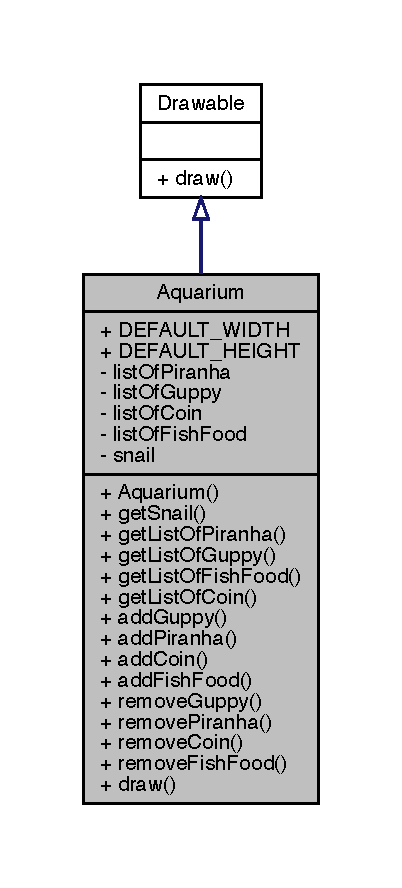
\includegraphics[width=193pt]{class_aquarium__inherit__graph}
\end{center}
\end{figure}


Collaboration diagram for Aquarium\+:
\nopagebreak
\begin{figure}[H]
\begin{center}
\leavevmode
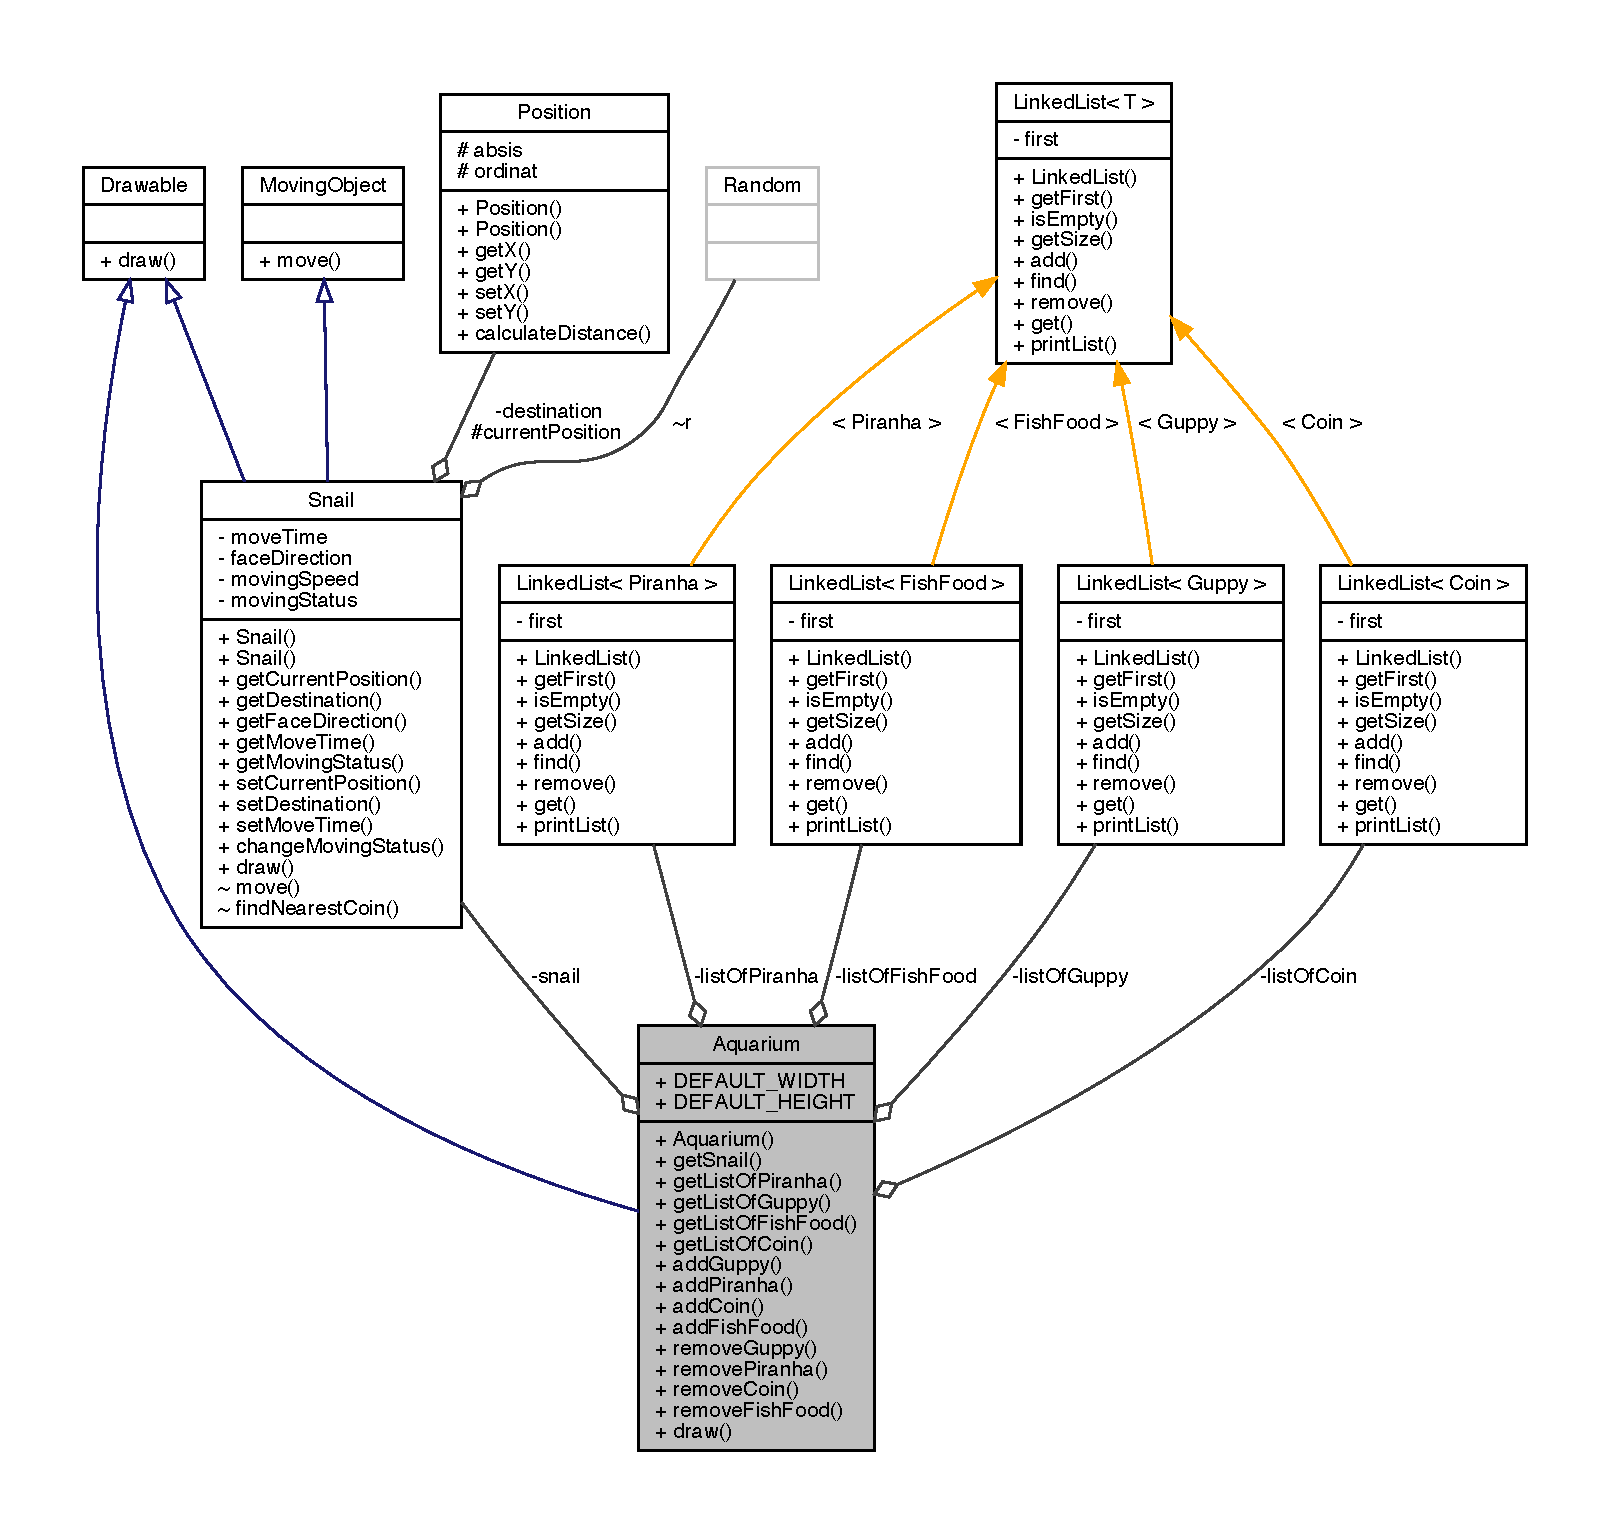
\includegraphics[width=350pt]{class_aquarium__coll__graph}
\end{center}
\end{figure}
\subsection*{Public Member Functions}
\begin{DoxyCompactItemize}
\item 
\mbox{\hyperlink{class_aquarium_a173f8b85de9d2f61c02d13ebdc05026c}{Aquarium}} ()
\item 
\mbox{\hyperlink{class_snail}{Snail}} \mbox{\hyperlink{class_aquarium_ac00cb1b361c2b368370f3fd1225ff296}{get\+Snail}} ()
\item 
\mbox{\hyperlink{class_linked_list}{Linked\+List}}$<$ \mbox{\hyperlink{class_piranha}{Piranha}} $>$ \mbox{\hyperlink{class_aquarium_a2427d901ce170774e36ca1a8ecbe8f4b}{get\+List\+Of\+Piranha}} ()
\item 
\mbox{\hyperlink{class_linked_list}{Linked\+List}}$<$ \mbox{\hyperlink{class_guppy}{Guppy}} $>$ \mbox{\hyperlink{class_aquarium_a411ebb8e3ada997747567f59da24a020}{get\+List\+Of\+Guppy}} ()
\item 
\mbox{\hyperlink{class_linked_list}{Linked\+List}}$<$ \mbox{\hyperlink{class_fish_food}{Fish\+Food}} $>$ \mbox{\hyperlink{class_aquarium_acfab5e8dd55512337ae91cf923e565e6}{get\+List\+Of\+Fish\+Food}} ()
\item 
\mbox{\hyperlink{class_linked_list}{Linked\+List}}$<$ \mbox{\hyperlink{class_coin}{Coin}} $>$ \mbox{\hyperlink{class_aquarium_a9b0dec4c194324e6095b81262b042460}{get\+List\+Of\+Coin}} ()
\item 
void \mbox{\hyperlink{class_aquarium_a4deb3514c2e387b5d3e33424c18144c1}{add\+Guppy}} (\mbox{\hyperlink{class_guppy}{Guppy}} guppy)
\item 
void \mbox{\hyperlink{class_aquarium_a30faca886e988aa80f512086cd817588}{add\+Piranha}} (\mbox{\hyperlink{class_piranha}{Piranha}} piranha)
\item 
void \mbox{\hyperlink{class_aquarium_a8b33e39d738b36ef732fefbcfdbd9ab1}{add\+Coin}} (\mbox{\hyperlink{class_coin}{Coin}} coin)
\item 
void \mbox{\hyperlink{class_aquarium_a36020897197a43587bcedc6aaf617a0f}{add\+Fish\+Food}} (\mbox{\hyperlink{class_fish_food}{Fish\+Food}} food)
\item 
void \mbox{\hyperlink{class_aquarium_a08f7e597644cad58198ed84d431f4599}{remove\+Guppy}} (\mbox{\hyperlink{class_guppy}{Guppy}} guppy)
\item 
void \mbox{\hyperlink{class_aquarium_ae0e31a6266a7d847f2bcaf1ee77fe5b4}{remove\+Piranha}} (\mbox{\hyperlink{class_piranha}{Piranha}} piranha)
\item 
void \mbox{\hyperlink{class_aquarium_af6f2d1079224c08a0ff7d376ea04c732}{remove\+Coin}} (\mbox{\hyperlink{class_coin}{Coin}} coin)
\item 
void \mbox{\hyperlink{class_aquarium_a6c1a0d6a0cc7cd4604dfce22706f57ca}{remove\+Fish\+Food}} (\mbox{\hyperlink{class_fish_food}{Fish\+Food}} food)
\item 
void \mbox{\hyperlink{class_aquarium_af6a186c92c1f91f92ae382416b77d3c3}{draw}} (Graphics g, Toolkit t)
\end{DoxyCompactItemize}
\subsection*{Static Public Attributes}
\begin{DoxyCompactItemize}
\item 
static final int \mbox{\hyperlink{class_aquarium_a1434fb962b1f08bc4f597b14b15431bb}{D\+E\+F\+A\+U\+L\+T\+\_\+\+W\+I\+D\+TH}} = 650
\item 
static final int \mbox{\hyperlink{class_aquarium_a65cefc6de1690de8d537d19940bd8e01}{D\+E\+F\+A\+U\+L\+T\+\_\+\+H\+E\+I\+G\+HT}} = 508
\end{DoxyCompactItemize}
\subsection*{Private Attributes}
\begin{DoxyCompactItemize}
\item 
\mbox{\hyperlink{class_linked_list}{Linked\+List}}$<$ \mbox{\hyperlink{class_piranha}{Piranha}} $>$ \mbox{\hyperlink{class_aquarium_a21cb53c360484e651bde146b4645ca4a}{list\+Of\+Piranha}}
\item 
\mbox{\hyperlink{class_linked_list}{Linked\+List}}$<$ \mbox{\hyperlink{class_guppy}{Guppy}} $>$ \mbox{\hyperlink{class_aquarium_a020d5cd650fba937c38d7b25aed6effd}{list\+Of\+Guppy}}
\item 
\mbox{\hyperlink{class_linked_list}{Linked\+List}}$<$ \mbox{\hyperlink{class_coin}{Coin}} $>$ \mbox{\hyperlink{class_aquarium_a26c4ffdfd5ee2c9819a1125ad5c077d1}{list\+Of\+Coin}}
\item 
\mbox{\hyperlink{class_linked_list}{Linked\+List}}$<$ \mbox{\hyperlink{class_fish_food}{Fish\+Food}} $>$ \mbox{\hyperlink{class_aquarium_a17e3ff17ab95a5d3d45780eae72448c7}{list\+Of\+Fish\+Food}}
\item 
\mbox{\hyperlink{class_snail}{Snail}} \mbox{\hyperlink{class_aquarium_a181508459b3020488aa97664daeb79ac}{snail}}
\end{DoxyCompactItemize}


\subsection{Detailed Description}
Represents an aquarium. \begin{DoxyVersion}{Version}
1.\+0. 
\end{DoxyVersion}


\subsection{Constructor \& Destructor Documentation}
\mbox{\Hypertarget{class_aquarium_a173f8b85de9d2f61c02d13ebdc05026c}\label{class_aquarium_a173f8b85de9d2f61c02d13ebdc05026c}} 
\index{Aquarium@{Aquarium}!Aquarium@{Aquarium}}
\index{Aquarium@{Aquarium}!Aquarium@{Aquarium}}
\subsubsection{\texorpdfstring{Aquarium()}{Aquarium()}}
{\footnotesize\ttfamily Aquarium.\+Aquarium (\begin{DoxyParamCaption}{ }\end{DoxyParamCaption})\hspace{0.3cm}{\ttfamily [inline]}}

\mbox{\hyperlink{class_aquarium}{Aquarium}} Constructor. 

\subsection{Member Function Documentation}
\mbox{\Hypertarget{class_aquarium_a8b33e39d738b36ef732fefbcfdbd9ab1}\label{class_aquarium_a8b33e39d738b36ef732fefbcfdbd9ab1}} 
\index{Aquarium@{Aquarium}!add\+Coin@{add\+Coin}}
\index{add\+Coin@{add\+Coin}!Aquarium@{Aquarium}}
\subsubsection{\texorpdfstring{add\+Coin()}{addCoin()}}
{\footnotesize\ttfamily void Aquarium.\+add\+Coin (\begin{DoxyParamCaption}\item[{\mbox{\hyperlink{class_coin}{Coin}}}]{coin }\end{DoxyParamCaption})\hspace{0.3cm}{\ttfamily [inline]}}

add coin to list\+Of\+Coin. 
\begin{DoxyParams}{Parameters}
{\em coin} & \mbox{\hyperlink{class_coin}{Coin}} object to add. \\
\hline
\end{DoxyParams}
Here is the call graph for this function\+:
\nopagebreak
\begin{figure}[H]
\begin{center}
\leavevmode
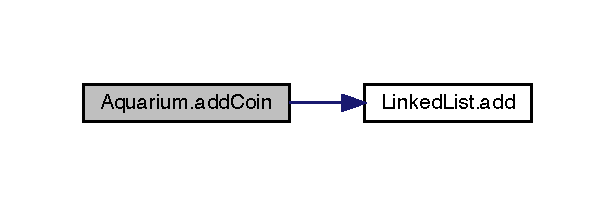
\includegraphics[width=295pt]{class_aquarium_a8b33e39d738b36ef732fefbcfdbd9ab1_cgraph}
\end{center}
\end{figure}
\mbox{\Hypertarget{class_aquarium_a36020897197a43587bcedc6aaf617a0f}\label{class_aquarium_a36020897197a43587bcedc6aaf617a0f}} 
\index{Aquarium@{Aquarium}!add\+Fish\+Food@{add\+Fish\+Food}}
\index{add\+Fish\+Food@{add\+Fish\+Food}!Aquarium@{Aquarium}}
\subsubsection{\texorpdfstring{add\+Fish\+Food()}{addFishFood()}}
{\footnotesize\ttfamily void Aquarium.\+add\+Fish\+Food (\begin{DoxyParamCaption}\item[{\mbox{\hyperlink{class_fish_food}{Fish\+Food}}}]{food }\end{DoxyParamCaption})\hspace{0.3cm}{\ttfamily [inline]}}

add food to list\+Of\+Fish\+Food. 
\begin{DoxyParams}{Parameters}
{\em food} & \mbox{\hyperlink{class_fish_food}{Fish\+Food}} object to add. \\
\hline
\end{DoxyParams}
Here is the call graph for this function\+:
\nopagebreak
\begin{figure}[H]
\begin{center}
\leavevmode
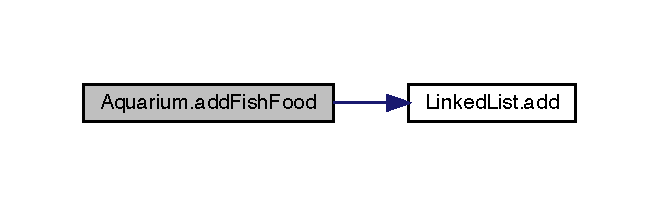
\includegraphics[width=316pt]{class_aquarium_a36020897197a43587bcedc6aaf617a0f_cgraph}
\end{center}
\end{figure}
\mbox{\Hypertarget{class_aquarium_a4deb3514c2e387b5d3e33424c18144c1}\label{class_aquarium_a4deb3514c2e387b5d3e33424c18144c1}} 
\index{Aquarium@{Aquarium}!add\+Guppy@{add\+Guppy}}
\index{add\+Guppy@{add\+Guppy}!Aquarium@{Aquarium}}
\subsubsection{\texorpdfstring{add\+Guppy()}{addGuppy()}}
{\footnotesize\ttfamily void Aquarium.\+add\+Guppy (\begin{DoxyParamCaption}\item[{\mbox{\hyperlink{class_guppy}{Guppy}}}]{guppy }\end{DoxyParamCaption})\hspace{0.3cm}{\ttfamily [inline]}}

add guppy to list\+Ofguppy. 
\begin{DoxyParams}{Parameters}
{\em guppy} & \mbox{\hyperlink{class_guppy}{Guppy}} object to add. \\
\hline
\end{DoxyParams}
Here is the call graph for this function\+:
\nopagebreak
\begin{figure}[H]
\begin{center}
\leavevmode
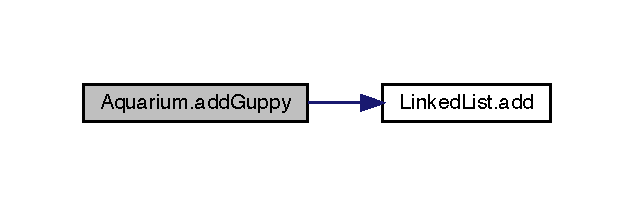
\includegraphics[width=304pt]{class_aquarium_a4deb3514c2e387b5d3e33424c18144c1_cgraph}
\end{center}
\end{figure}
\mbox{\Hypertarget{class_aquarium_a30faca886e988aa80f512086cd817588}\label{class_aquarium_a30faca886e988aa80f512086cd817588}} 
\index{Aquarium@{Aquarium}!add\+Piranha@{add\+Piranha}}
\index{add\+Piranha@{add\+Piranha}!Aquarium@{Aquarium}}
\subsubsection{\texorpdfstring{add\+Piranha()}{addPiranha()}}
{\footnotesize\ttfamily void Aquarium.\+add\+Piranha (\begin{DoxyParamCaption}\item[{\mbox{\hyperlink{class_piranha}{Piranha}}}]{piranha }\end{DoxyParamCaption})\hspace{0.3cm}{\ttfamily [inline]}}

add piranha to list\+Of\+Piranha. 
\begin{DoxyParams}{Parameters}
{\em piranha} & \mbox{\hyperlink{class_piranha}{Piranha}} object to add. \\
\hline
\end{DoxyParams}
Here is the call graph for this function\+:
\nopagebreak
\begin{figure}[H]
\begin{center}
\leavevmode
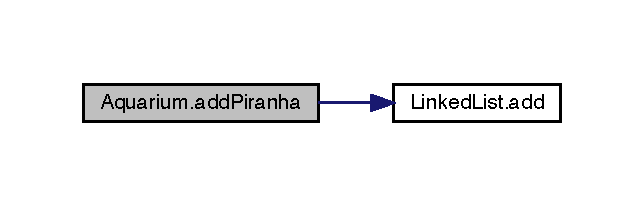
\includegraphics[width=309pt]{class_aquarium_a30faca886e988aa80f512086cd817588_cgraph}
\end{center}
\end{figure}
\mbox{\Hypertarget{class_aquarium_af6a186c92c1f91f92ae382416b77d3c3}\label{class_aquarium_af6a186c92c1f91f92ae382416b77d3c3}} 
\index{Aquarium@{Aquarium}!draw@{draw}}
\index{draw@{draw}!Aquarium@{Aquarium}}
\subsubsection{\texorpdfstring{draw()}{draw()}}
{\footnotesize\ttfamily void Aquarium.\+draw (\begin{DoxyParamCaption}\item[{Graphics}]{g,  }\item[{Toolkit}]{t }\end{DoxyParamCaption})\hspace{0.3cm}{\ttfamily [inline]}}

draw to aquarium. 
\begin{DoxyParams}{Parameters}
{\em g} & Draw container. \\
\hline
{\em t} & Object to grab image. \\
\hline
\end{DoxyParams}


Implements \mbox{\hyperlink{interface_drawable_aaddafb212b3c8e60fcc742052570c893}{Drawable}}.

\mbox{\Hypertarget{class_aquarium_a9b0dec4c194324e6095b81262b042460}\label{class_aquarium_a9b0dec4c194324e6095b81262b042460}} 
\index{Aquarium@{Aquarium}!get\+List\+Of\+Coin@{get\+List\+Of\+Coin}}
\index{get\+List\+Of\+Coin@{get\+List\+Of\+Coin}!Aquarium@{Aquarium}}
\subsubsection{\texorpdfstring{get\+List\+Of\+Coin()}{getListOfCoin()}}
{\footnotesize\ttfamily \mbox{\hyperlink{class_linked_list}{Linked\+List}}$<$\mbox{\hyperlink{class_coin}{Coin}}$>$ Aquarium.\+get\+List\+Of\+Coin (\begin{DoxyParamCaption}{ }\end{DoxyParamCaption})\hspace{0.3cm}{\ttfamily [inline]}}

list\+Of\+Coin prop getter. \begin{DoxyReturn}{Returns}
object of class \mbox{\hyperlink{class_linked_list}{Linked\+List}} of \mbox{\hyperlink{class_coin}{Coin}}. 
\end{DoxyReturn}
\mbox{\Hypertarget{class_aquarium_acfab5e8dd55512337ae91cf923e565e6}\label{class_aquarium_acfab5e8dd55512337ae91cf923e565e6}} 
\index{Aquarium@{Aquarium}!get\+List\+Of\+Fish\+Food@{get\+List\+Of\+Fish\+Food}}
\index{get\+List\+Of\+Fish\+Food@{get\+List\+Of\+Fish\+Food}!Aquarium@{Aquarium}}
\subsubsection{\texorpdfstring{get\+List\+Of\+Fish\+Food()}{getListOfFishFood()}}
{\footnotesize\ttfamily \mbox{\hyperlink{class_linked_list}{Linked\+List}}$<$\mbox{\hyperlink{class_fish_food}{Fish\+Food}}$>$ Aquarium.\+get\+List\+Of\+Fish\+Food (\begin{DoxyParamCaption}{ }\end{DoxyParamCaption})\hspace{0.3cm}{\ttfamily [inline]}}

list\+Of\+Fish\+Food prop getter. \begin{DoxyReturn}{Returns}
object of class \mbox{\hyperlink{class_linked_list}{Linked\+List}} of \mbox{\hyperlink{class_fish_food}{Fish\+Food}}. 
\end{DoxyReturn}
\mbox{\Hypertarget{class_aquarium_a411ebb8e3ada997747567f59da24a020}\label{class_aquarium_a411ebb8e3ada997747567f59da24a020}} 
\index{Aquarium@{Aquarium}!get\+List\+Of\+Guppy@{get\+List\+Of\+Guppy}}
\index{get\+List\+Of\+Guppy@{get\+List\+Of\+Guppy}!Aquarium@{Aquarium}}
\subsubsection{\texorpdfstring{get\+List\+Of\+Guppy()}{getListOfGuppy()}}
{\footnotesize\ttfamily \mbox{\hyperlink{class_linked_list}{Linked\+List}}$<$\mbox{\hyperlink{class_guppy}{Guppy}}$>$ Aquarium.\+get\+List\+Of\+Guppy (\begin{DoxyParamCaption}{ }\end{DoxyParamCaption})\hspace{0.3cm}{\ttfamily [inline]}}

list\+Of\+Guppy prop getter. \begin{DoxyReturn}{Returns}
object of class \mbox{\hyperlink{class_linked_list}{Linked\+List}} of \mbox{\hyperlink{class_guppy}{Guppy}}. 
\end{DoxyReturn}
\mbox{\Hypertarget{class_aquarium_a2427d901ce170774e36ca1a8ecbe8f4b}\label{class_aquarium_a2427d901ce170774e36ca1a8ecbe8f4b}} 
\index{Aquarium@{Aquarium}!get\+List\+Of\+Piranha@{get\+List\+Of\+Piranha}}
\index{get\+List\+Of\+Piranha@{get\+List\+Of\+Piranha}!Aquarium@{Aquarium}}
\subsubsection{\texorpdfstring{get\+List\+Of\+Piranha()}{getListOfPiranha()}}
{\footnotesize\ttfamily \mbox{\hyperlink{class_linked_list}{Linked\+List}}$<$\mbox{\hyperlink{class_piranha}{Piranha}}$>$ Aquarium.\+get\+List\+Of\+Piranha (\begin{DoxyParamCaption}{ }\end{DoxyParamCaption})\hspace{0.3cm}{\ttfamily [inline]}}

list\+Of\+Piranha prop getter. \begin{DoxyReturn}{Returns}
object of class \mbox{\hyperlink{class_linked_list}{Linked\+List}} of \mbox{\hyperlink{class_piranha}{Piranha}}. 
\end{DoxyReturn}
\mbox{\Hypertarget{class_aquarium_ac00cb1b361c2b368370f3fd1225ff296}\label{class_aquarium_ac00cb1b361c2b368370f3fd1225ff296}} 
\index{Aquarium@{Aquarium}!get\+Snail@{get\+Snail}}
\index{get\+Snail@{get\+Snail}!Aquarium@{Aquarium}}
\subsubsection{\texorpdfstring{get\+Snail()}{getSnail()}}
{\footnotesize\ttfamily \mbox{\hyperlink{class_snail}{Snail}} Aquarium.\+get\+Snail (\begin{DoxyParamCaption}{ }\end{DoxyParamCaption})\hspace{0.3cm}{\ttfamily [inline]}}

\mbox{\hyperlink{class_snail}{Snail}} prop getter. \begin{DoxyReturn}{Returns}
object of class \mbox{\hyperlink{class_snail}{Snail}}. 
\end{DoxyReturn}
\mbox{\Hypertarget{class_aquarium_af6f2d1079224c08a0ff7d376ea04c732}\label{class_aquarium_af6f2d1079224c08a0ff7d376ea04c732}} 
\index{Aquarium@{Aquarium}!remove\+Coin@{remove\+Coin}}
\index{remove\+Coin@{remove\+Coin}!Aquarium@{Aquarium}}
\subsubsection{\texorpdfstring{remove\+Coin()}{removeCoin()}}
{\footnotesize\ttfamily void Aquarium.\+remove\+Coin (\begin{DoxyParamCaption}\item[{\mbox{\hyperlink{class_coin}{Coin}}}]{coin }\end{DoxyParamCaption})\hspace{0.3cm}{\ttfamily [inline]}}

remove coin from list\+Of\+Coin. 
\begin{DoxyParams}{Parameters}
{\em coin} & \mbox{\hyperlink{class_coin}{Coin}} object to remove. \\
\hline
\end{DoxyParams}
Here is the call graph for this function\+:
\nopagebreak
\begin{figure}[H]
\begin{center}
\leavevmode
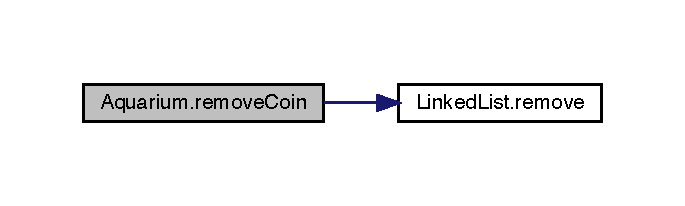
\includegraphics[width=329pt]{class_aquarium_af6f2d1079224c08a0ff7d376ea04c732_cgraph}
\end{center}
\end{figure}
\mbox{\Hypertarget{class_aquarium_a6c1a0d6a0cc7cd4604dfce22706f57ca}\label{class_aquarium_a6c1a0d6a0cc7cd4604dfce22706f57ca}} 
\index{Aquarium@{Aquarium}!remove\+Fish\+Food@{remove\+Fish\+Food}}
\index{remove\+Fish\+Food@{remove\+Fish\+Food}!Aquarium@{Aquarium}}
\subsubsection{\texorpdfstring{remove\+Fish\+Food()}{removeFishFood()}}
{\footnotesize\ttfamily void Aquarium.\+remove\+Fish\+Food (\begin{DoxyParamCaption}\item[{\mbox{\hyperlink{class_fish_food}{Fish\+Food}}}]{food }\end{DoxyParamCaption})\hspace{0.3cm}{\ttfamily [inline]}}

remove food from list\+Of\+Fish\+Food. 
\begin{DoxyParams}{Parameters}
{\em food} & \mbox{\hyperlink{class_fish_food}{Fish\+Food}} object to remove. \\
\hline
\end{DoxyParams}
Here is the call graph for this function\+:
\nopagebreak
\begin{figure}[H]
\begin{center}
\leavevmode
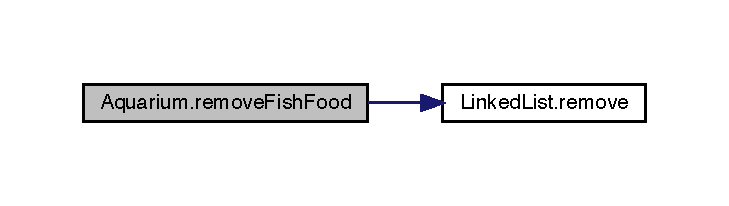
\includegraphics[width=350pt]{class_aquarium_a6c1a0d6a0cc7cd4604dfce22706f57ca_cgraph}
\end{center}
\end{figure}
\mbox{\Hypertarget{class_aquarium_a08f7e597644cad58198ed84d431f4599}\label{class_aquarium_a08f7e597644cad58198ed84d431f4599}} 
\index{Aquarium@{Aquarium}!remove\+Guppy@{remove\+Guppy}}
\index{remove\+Guppy@{remove\+Guppy}!Aquarium@{Aquarium}}
\subsubsection{\texorpdfstring{remove\+Guppy()}{removeGuppy()}}
{\footnotesize\ttfamily void Aquarium.\+remove\+Guppy (\begin{DoxyParamCaption}\item[{\mbox{\hyperlink{class_guppy}{Guppy}}}]{guppy }\end{DoxyParamCaption})\hspace{0.3cm}{\ttfamily [inline]}}

remove guppy from list\+Ofguppy. 
\begin{DoxyParams}{Parameters}
{\em guppy} & \mbox{\hyperlink{class_guppy}{Guppy}} object to remove. \\
\hline
\end{DoxyParams}
Here is the call graph for this function\+:
\nopagebreak
\begin{figure}[H]
\begin{center}
\leavevmode
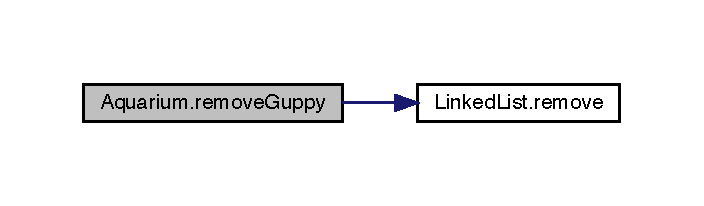
\includegraphics[width=338pt]{class_aquarium_a08f7e597644cad58198ed84d431f4599_cgraph}
\end{center}
\end{figure}
\mbox{\Hypertarget{class_aquarium_ae0e31a6266a7d847f2bcaf1ee77fe5b4}\label{class_aquarium_ae0e31a6266a7d847f2bcaf1ee77fe5b4}} 
\index{Aquarium@{Aquarium}!remove\+Piranha@{remove\+Piranha}}
\index{remove\+Piranha@{remove\+Piranha}!Aquarium@{Aquarium}}
\subsubsection{\texorpdfstring{remove\+Piranha()}{removePiranha()}}
{\footnotesize\ttfamily void Aquarium.\+remove\+Piranha (\begin{DoxyParamCaption}\item[{\mbox{\hyperlink{class_piranha}{Piranha}}}]{piranha }\end{DoxyParamCaption})\hspace{0.3cm}{\ttfamily [inline]}}

remove piranha from list\+Of\+Piranha. 
\begin{DoxyParams}{Parameters}
{\em piranha} & \mbox{\hyperlink{class_piranha}{Piranha}} object to remove. \\
\hline
\end{DoxyParams}
Here is the call graph for this function\+:
\nopagebreak
\begin{figure}[H]
\begin{center}
\leavevmode
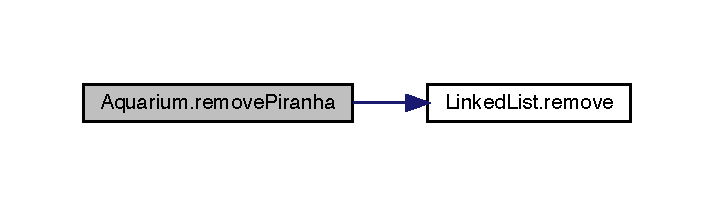
\includegraphics[width=343pt]{class_aquarium_ae0e31a6266a7d847f2bcaf1ee77fe5b4_cgraph}
\end{center}
\end{figure}


\subsection{Member Data Documentation}
\mbox{\Hypertarget{class_aquarium_a65cefc6de1690de8d537d19940bd8e01}\label{class_aquarium_a65cefc6de1690de8d537d19940bd8e01}} 
\index{Aquarium@{Aquarium}!D\+E\+F\+A\+U\+L\+T\+\_\+\+H\+E\+I\+G\+HT@{D\+E\+F\+A\+U\+L\+T\+\_\+\+H\+E\+I\+G\+HT}}
\index{D\+E\+F\+A\+U\+L\+T\+\_\+\+H\+E\+I\+G\+HT@{D\+E\+F\+A\+U\+L\+T\+\_\+\+H\+E\+I\+G\+HT}!Aquarium@{Aquarium}}
\subsubsection{\texorpdfstring{D\+E\+F\+A\+U\+L\+T\+\_\+\+H\+E\+I\+G\+HT}{DEFAULT\_HEIGHT}}
{\footnotesize\ttfamily final int Aquarium.\+D\+E\+F\+A\+U\+L\+T\+\_\+\+H\+E\+I\+G\+HT = 508\hspace{0.3cm}{\ttfamily [static]}}

Max Height of the app window . \mbox{\Hypertarget{class_aquarium_a1434fb962b1f08bc4f597b14b15431bb}\label{class_aquarium_a1434fb962b1f08bc4f597b14b15431bb}} 
\index{Aquarium@{Aquarium}!D\+E\+F\+A\+U\+L\+T\+\_\+\+W\+I\+D\+TH@{D\+E\+F\+A\+U\+L\+T\+\_\+\+W\+I\+D\+TH}}
\index{D\+E\+F\+A\+U\+L\+T\+\_\+\+W\+I\+D\+TH@{D\+E\+F\+A\+U\+L\+T\+\_\+\+W\+I\+D\+TH}!Aquarium@{Aquarium}}
\subsubsection{\texorpdfstring{D\+E\+F\+A\+U\+L\+T\+\_\+\+W\+I\+D\+TH}{DEFAULT\_WIDTH}}
{\footnotesize\ttfamily final int Aquarium.\+D\+E\+F\+A\+U\+L\+T\+\_\+\+W\+I\+D\+TH = 650\hspace{0.3cm}{\ttfamily [static]}}

Max Width of the app window . \mbox{\Hypertarget{class_aquarium_a26c4ffdfd5ee2c9819a1125ad5c077d1}\label{class_aquarium_a26c4ffdfd5ee2c9819a1125ad5c077d1}} 
\index{Aquarium@{Aquarium}!list\+Of\+Coin@{list\+Of\+Coin}}
\index{list\+Of\+Coin@{list\+Of\+Coin}!Aquarium@{Aquarium}}
\subsubsection{\texorpdfstring{list\+Of\+Coin}{listOfCoin}}
{\footnotesize\ttfamily \mbox{\hyperlink{class_linked_list}{Linked\+List}}$<$\mbox{\hyperlink{class_coin}{Coin}}$>$ Aquarium.\+list\+Of\+Coin\hspace{0.3cm}{\ttfamily [private]}}

\mbox{\Hypertarget{class_aquarium_a17e3ff17ab95a5d3d45780eae72448c7}\label{class_aquarium_a17e3ff17ab95a5d3d45780eae72448c7}} 
\index{Aquarium@{Aquarium}!list\+Of\+Fish\+Food@{list\+Of\+Fish\+Food}}
\index{list\+Of\+Fish\+Food@{list\+Of\+Fish\+Food}!Aquarium@{Aquarium}}
\subsubsection{\texorpdfstring{list\+Of\+Fish\+Food}{listOfFishFood}}
{\footnotesize\ttfamily \mbox{\hyperlink{class_linked_list}{Linked\+List}}$<$\mbox{\hyperlink{class_fish_food}{Fish\+Food}}$>$ Aquarium.\+list\+Of\+Fish\+Food\hspace{0.3cm}{\ttfamily [private]}}

\mbox{\Hypertarget{class_aquarium_a020d5cd650fba937c38d7b25aed6effd}\label{class_aquarium_a020d5cd650fba937c38d7b25aed6effd}} 
\index{Aquarium@{Aquarium}!list\+Of\+Guppy@{list\+Of\+Guppy}}
\index{list\+Of\+Guppy@{list\+Of\+Guppy}!Aquarium@{Aquarium}}
\subsubsection{\texorpdfstring{list\+Of\+Guppy}{listOfGuppy}}
{\footnotesize\ttfamily \mbox{\hyperlink{class_linked_list}{Linked\+List}}$<$\mbox{\hyperlink{class_guppy}{Guppy}}$>$ Aquarium.\+list\+Of\+Guppy\hspace{0.3cm}{\ttfamily [private]}}

\mbox{\Hypertarget{class_aquarium_a21cb53c360484e651bde146b4645ca4a}\label{class_aquarium_a21cb53c360484e651bde146b4645ca4a}} 
\index{Aquarium@{Aquarium}!list\+Of\+Piranha@{list\+Of\+Piranha}}
\index{list\+Of\+Piranha@{list\+Of\+Piranha}!Aquarium@{Aquarium}}
\subsubsection{\texorpdfstring{list\+Of\+Piranha}{listOfPiranha}}
{\footnotesize\ttfamily \mbox{\hyperlink{class_linked_list}{Linked\+List}}$<$\mbox{\hyperlink{class_piranha}{Piranha}}$>$ Aquarium.\+list\+Of\+Piranha\hspace{0.3cm}{\ttfamily [private]}}

\mbox{\Hypertarget{class_aquarium_a181508459b3020488aa97664daeb79ac}\label{class_aquarium_a181508459b3020488aa97664daeb79ac}} 
\index{Aquarium@{Aquarium}!snail@{snail}}
\index{snail@{snail}!Aquarium@{Aquarium}}
\subsubsection{\texorpdfstring{snail}{snail}}
{\footnotesize\ttfamily \mbox{\hyperlink{class_snail}{Snail}} Aquarium.\+snail\hspace{0.3cm}{\ttfamily [private]}}



The documentation for this class was generated from the following file\+:\begin{DoxyCompactItemize}
\item 
\mbox{\hyperlink{_aquarium_8java}{Aquarium.\+java}}\end{DoxyCompactItemize}

\hypertarget{class_coin}{}\section{Coin Class Reference}
\label{class_coin}\index{Coin@{Coin}}


Inheritance diagram for Coin\+:
\nopagebreak
\begin{figure}[H]
\begin{center}
\leavevmode
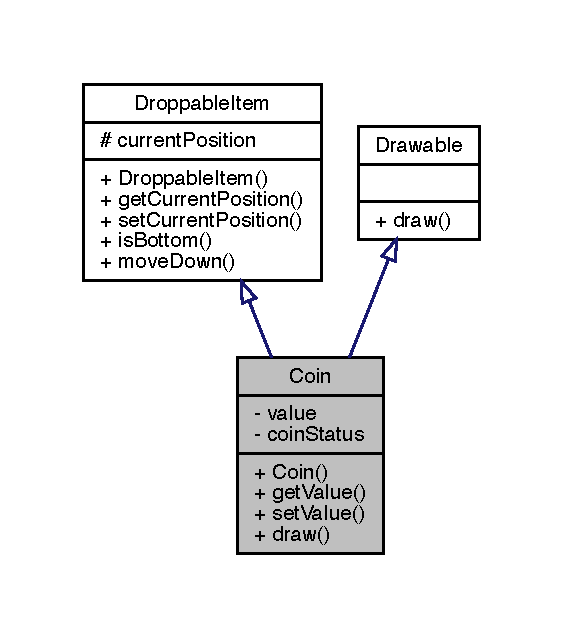
\includegraphics[width=270pt]{class_coin__inherit__graph}
\end{center}
\end{figure}


Collaboration diagram for Coin\+:
\nopagebreak
\begin{figure}[H]
\begin{center}
\leavevmode
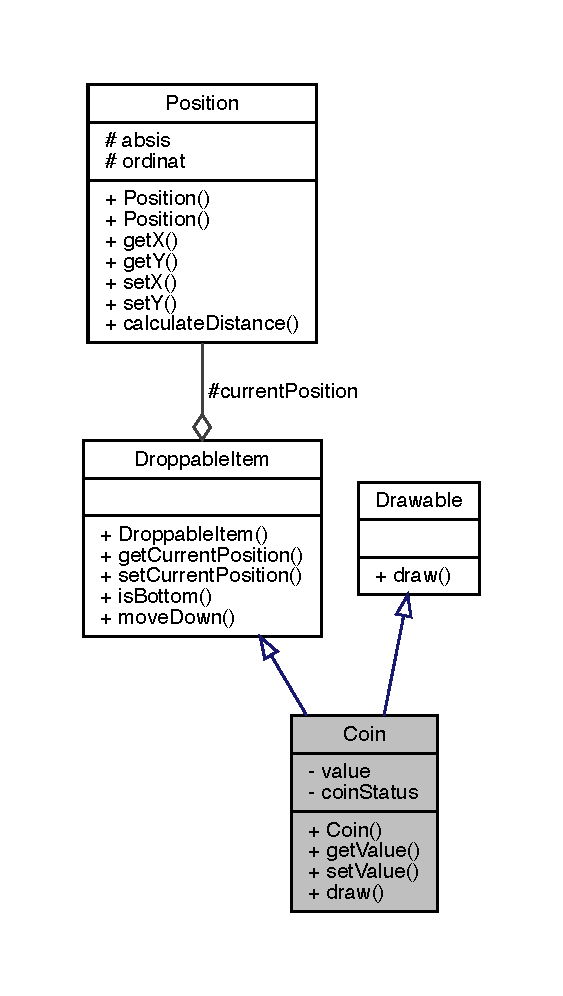
\includegraphics[width=270pt]{class_coin__coll__graph}
\end{center}
\end{figure}
\subsection*{Public Member Functions}
\begin{DoxyCompactItemize}
\item 
\mbox{\hyperlink{class_coin_ac75958fbac44671f534e83cde5df013b}{Coin}} (double \mbox{\hyperlink{class_coin_a1f18db679edab240c514b9a4dc47ec97}{value}}, \mbox{\hyperlink{class_position}{Position}} fish\+Position)
\item 
double \mbox{\hyperlink{class_coin_a420e22e4740d8836be0beb3678bc6fe0}{get\+Value}} ()
\item 
void \mbox{\hyperlink{class_coin_a4f3abfae192ec4fdf21389f41f799c5d}{set\+Value}} (double \mbox{\hyperlink{class_coin_a1f18db679edab240c514b9a4dc47ec97}{value}})
\item 
void \mbox{\hyperlink{class_coin_ae0c35ffd80b39f26f43d287da0565d0b}{draw}} (Graphics g, Toolkit t)
\end{DoxyCompactItemize}
\subsection*{Private Attributes}
\begin{DoxyCompactItemize}
\item 
double \mbox{\hyperlink{class_coin_a1f18db679edab240c514b9a4dc47ec97}{value}}
\item 
double \mbox{\hyperlink{class_coin_abf41bb0f883b43451460f3021ec6eed9}{coin\+Status}}
\end{DoxyCompactItemize}
\subsection*{Additional Inherited Members}


\subsection{Detailed Description}
Represents a coin \begin{DoxyVersion}{Version}
1.\+0 
\end{DoxyVersion}


\subsection{Constructor \& Destructor Documentation}
\mbox{\Hypertarget{class_coin_ac75958fbac44671f534e83cde5df013b}\label{class_coin_ac75958fbac44671f534e83cde5df013b}} 
\index{Coin@{Coin}!Coin@{Coin}}
\index{Coin@{Coin}!Coin@{Coin}}
\subsubsection{\texorpdfstring{Coin()}{Coin()}}
{\footnotesize\ttfamily Coin.\+Coin (\begin{DoxyParamCaption}\item[{double}]{value,  }\item[{\mbox{\hyperlink{class_position}{Position}}}]{fish\+Position }\end{DoxyParamCaption})\hspace{0.3cm}{\ttfamily [inline]}}

constructor. 
\begin{DoxyParams}{Parameters}
{\em value} & value of coin. \\
\hline
{\em fish\+Position} & \mbox{\hyperlink{class_position}{Position}} of fish. \\
\hline
\end{DoxyParams}


\subsection{Member Function Documentation}
\mbox{\Hypertarget{class_coin_ae0c35ffd80b39f26f43d287da0565d0b}\label{class_coin_ae0c35ffd80b39f26f43d287da0565d0b}} 
\index{Coin@{Coin}!draw@{draw}}
\index{draw@{draw}!Coin@{Coin}}
\subsubsection{\texorpdfstring{draw()}{draw()}}
{\footnotesize\ttfamily void Coin.\+draw (\begin{DoxyParamCaption}\item[{Graphics}]{g,  }\item[{Toolkit}]{t }\end{DoxyParamCaption})\hspace{0.3cm}{\ttfamily [inline]}}

draw to aquarium 
\begin{DoxyParams}{Parameters}
{\em g} & Draw container. \\
\hline
{\em t} & Object to grab image. \\
\hline
\end{DoxyParams}


Implements \mbox{\hyperlink{interface_drawable_aaddafb212b3c8e60fcc742052570c893}{Drawable}}.

Here is the call graph for this function\+:
\nopagebreak
\begin{figure}[H]
\begin{center}
\leavevmode
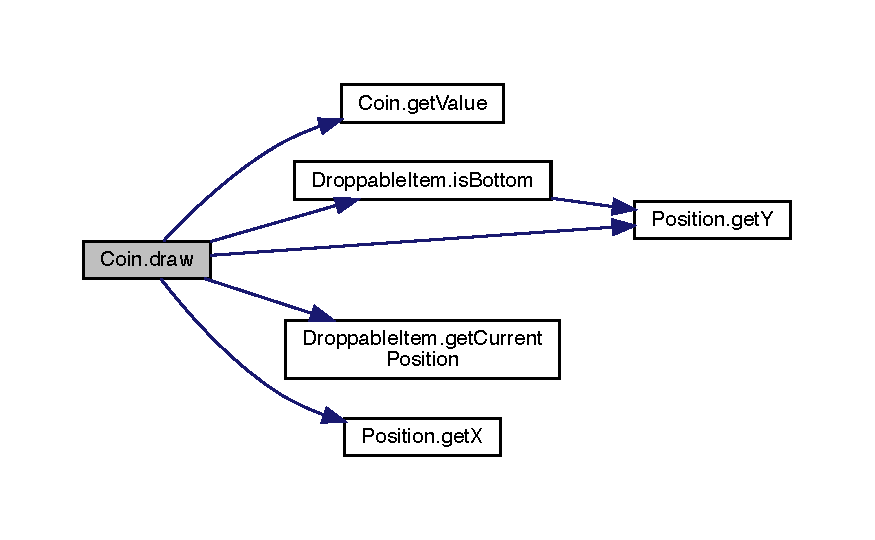
\includegraphics[width=350pt]{class_coin_ae0c35ffd80b39f26f43d287da0565d0b_cgraph}
\end{center}
\end{figure}
\mbox{\Hypertarget{class_coin_a420e22e4740d8836be0beb3678bc6fe0}\label{class_coin_a420e22e4740d8836be0beb3678bc6fe0}} 
\index{Coin@{Coin}!get\+Value@{get\+Value}}
\index{get\+Value@{get\+Value}!Coin@{Coin}}
\subsubsection{\texorpdfstring{get\+Value()}{getValue()}}
{\footnotesize\ttfamily double Coin.\+get\+Value (\begin{DoxyParamCaption}{ }\end{DoxyParamCaption})\hspace{0.3cm}{\ttfamily [inline]}}

value getter. \begin{DoxyReturn}{Returns}
value. 
\end{DoxyReturn}
\mbox{\Hypertarget{class_coin_a4f3abfae192ec4fdf21389f41f799c5d}\label{class_coin_a4f3abfae192ec4fdf21389f41f799c5d}} 
\index{Coin@{Coin}!set\+Value@{set\+Value}}
\index{set\+Value@{set\+Value}!Coin@{Coin}}
\subsubsection{\texorpdfstring{set\+Value()}{setValue()}}
{\footnotesize\ttfamily void Coin.\+set\+Value (\begin{DoxyParamCaption}\item[{double}]{value }\end{DoxyParamCaption})\hspace{0.3cm}{\ttfamily [inline]}}

value setter. 
\begin{DoxyParams}{Parameters}
{\em value} & value to be set. \\
\hline
\end{DoxyParams}


\subsection{Member Data Documentation}
\mbox{\Hypertarget{class_coin_abf41bb0f883b43451460f3021ec6eed9}\label{class_coin_abf41bb0f883b43451460f3021ec6eed9}} 
\index{Coin@{Coin}!coin\+Status@{coin\+Status}}
\index{coin\+Status@{coin\+Status}!Coin@{Coin}}
\subsubsection{\texorpdfstring{coin\+Status}{coinStatus}}
{\footnotesize\ttfamily double Coin.\+coin\+Status\hspace{0.3cm}{\ttfamily [private]}}

\mbox{\Hypertarget{class_coin_a1f18db679edab240c514b9a4dc47ec97}\label{class_coin_a1f18db679edab240c514b9a4dc47ec97}} 
\index{Coin@{Coin}!value@{value}}
\index{value@{value}!Coin@{Coin}}
\subsubsection{\texorpdfstring{value}{value}}
{\footnotesize\ttfamily double Coin.\+value\hspace{0.3cm}{\ttfamily [private]}}



The documentation for this class was generated from the following file\+:\begin{DoxyCompactItemize}
\item 
\mbox{\hyperlink{_coin_8java}{Coin.\+java}}\end{DoxyCompactItemize}

\hypertarget{class_controller}{}\section{Controller Class Reference}
\label{class_controller}\index{Controller@{Controller}}


Inheritance diagram for Controller\+:
\nopagebreak
\begin{figure}[H]
\begin{center}
\leavevmode
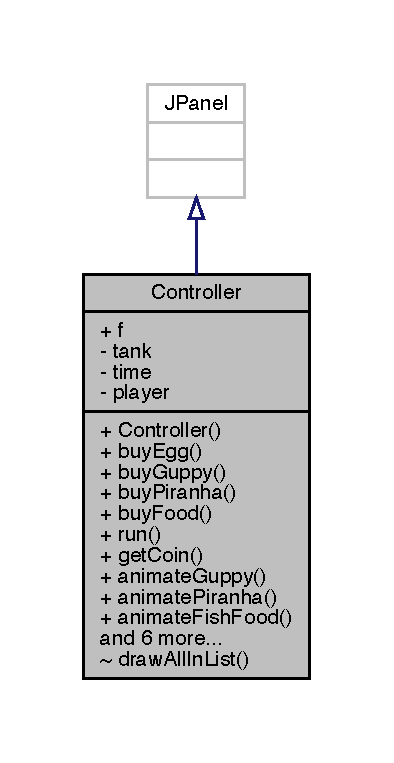
\includegraphics[width=189pt]{class_controller__inherit__graph}
\end{center}
\end{figure}


Collaboration diagram for Controller\+:
\nopagebreak
\begin{figure}[H]
\begin{center}
\leavevmode
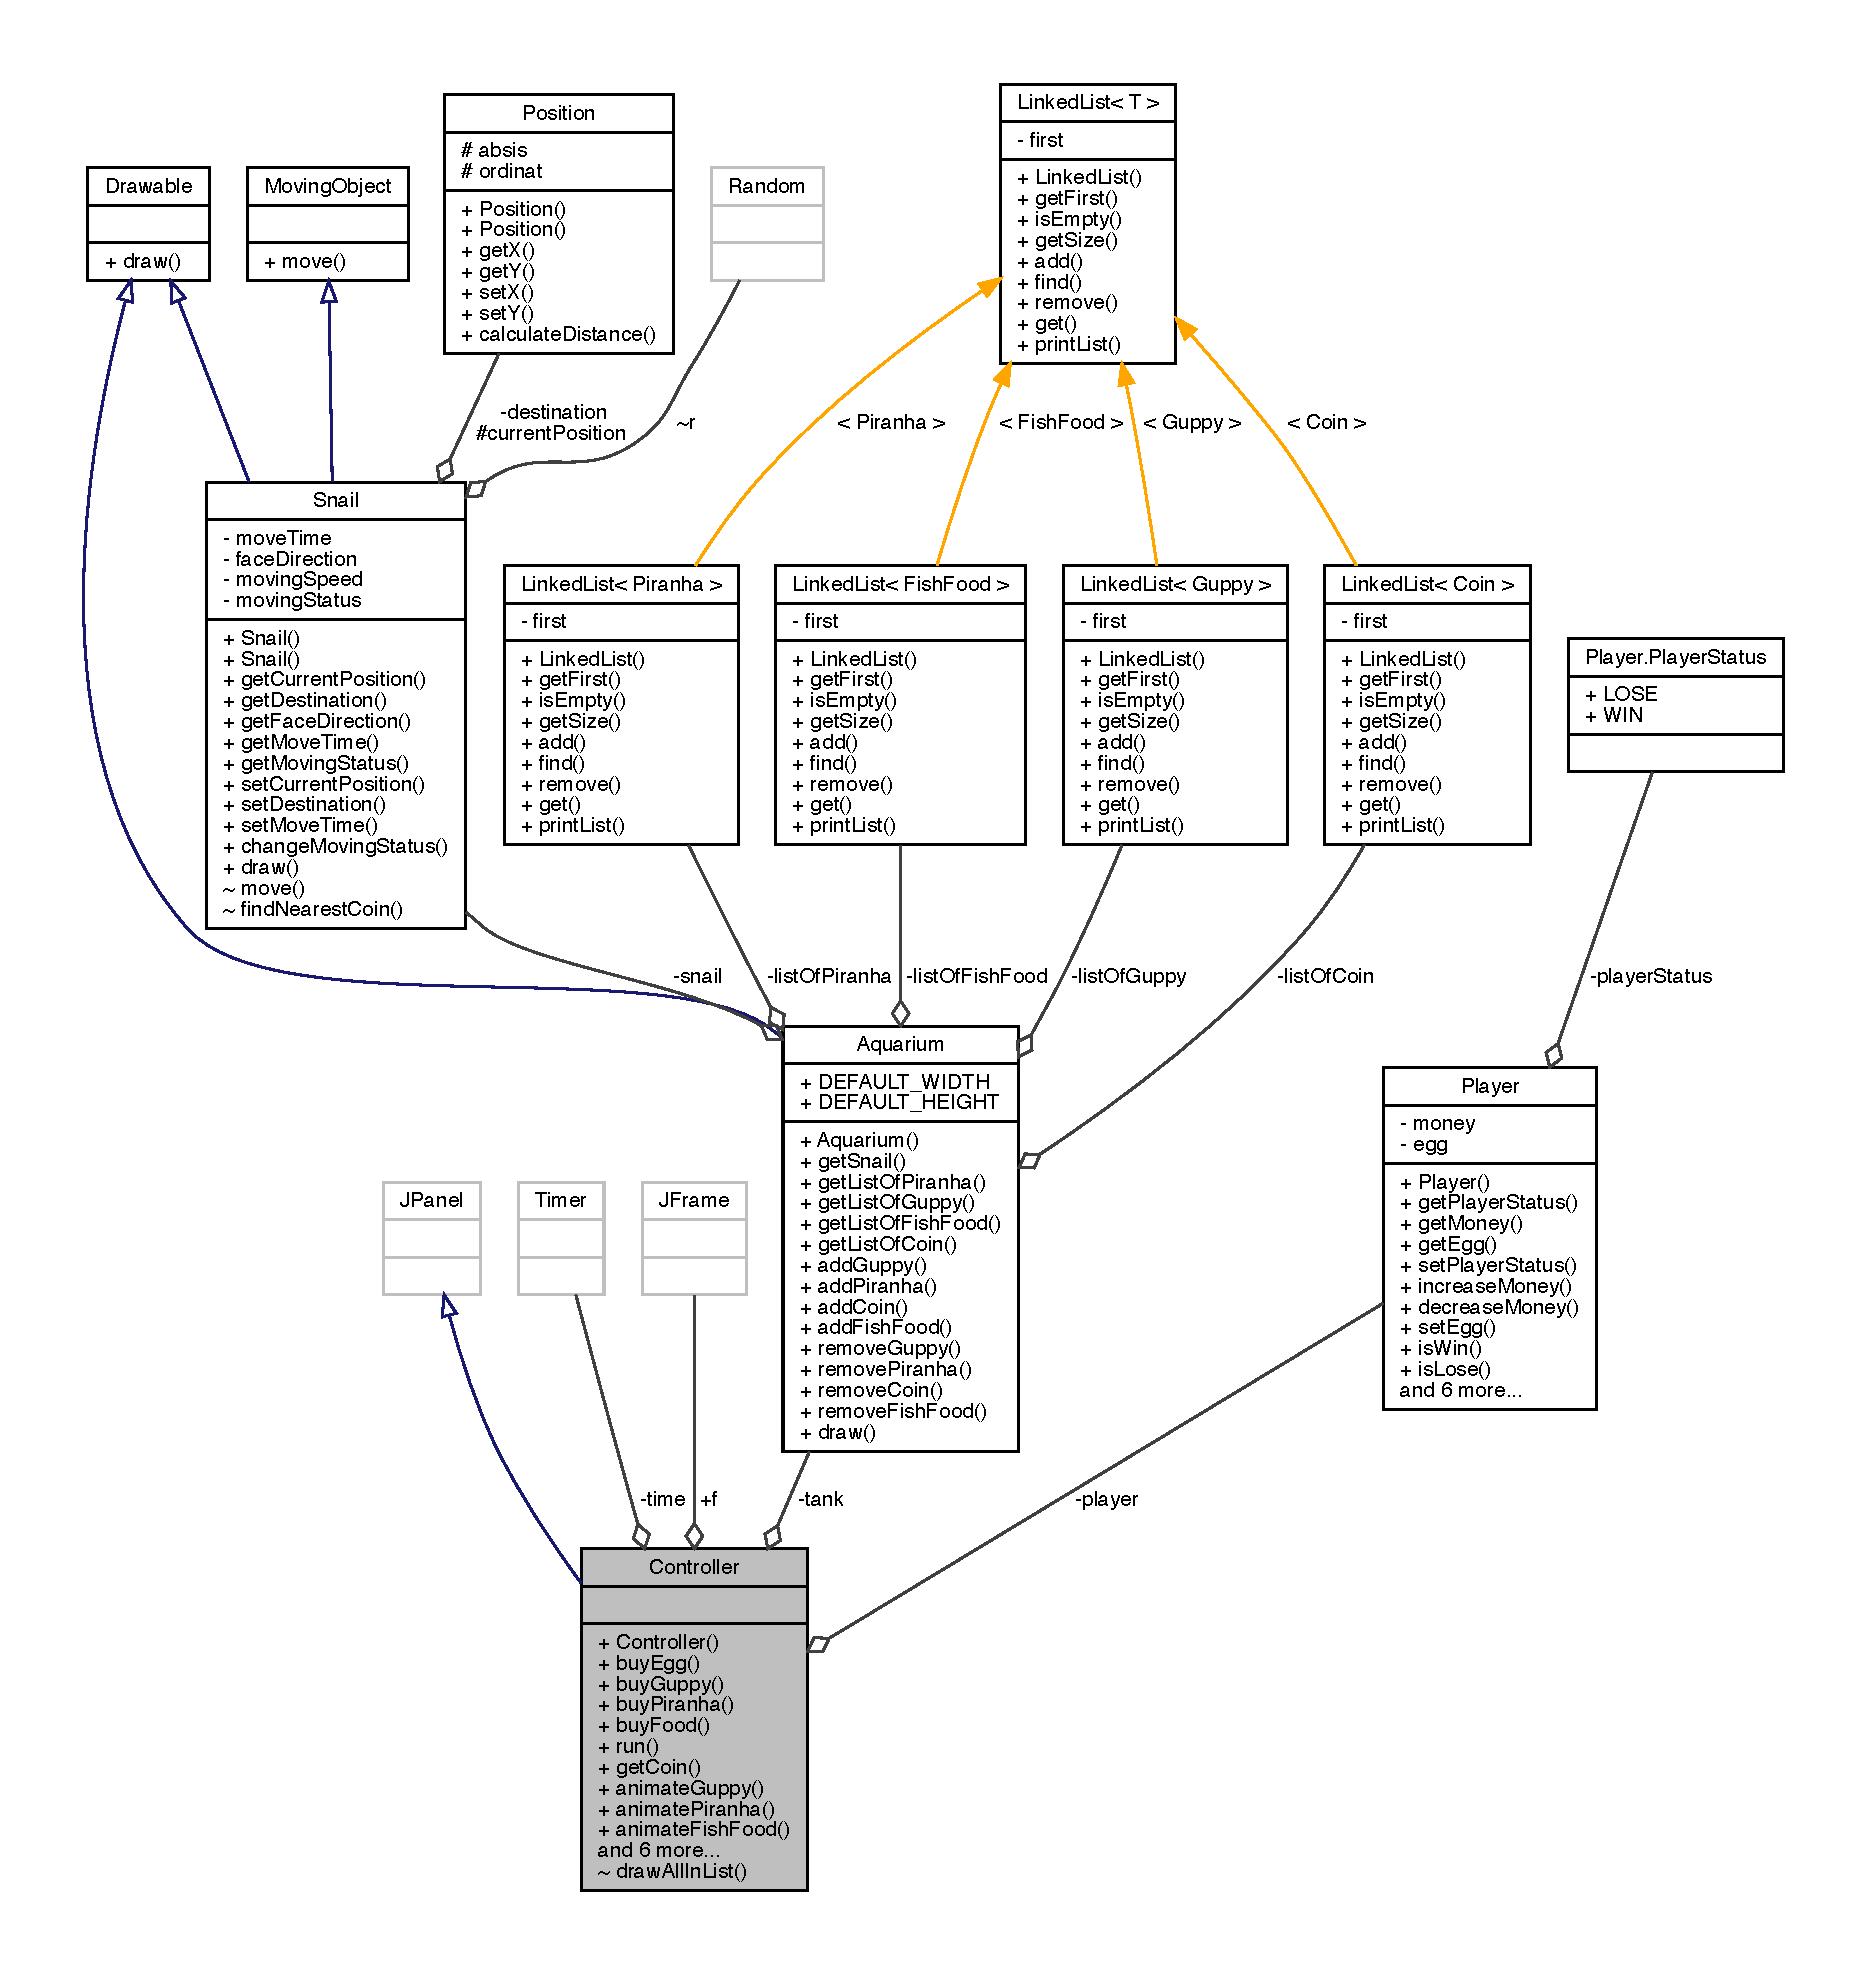
\includegraphics[width=350pt]{class_controller__coll__graph}
\end{center}
\end{figure}
\subsection*{Public Member Functions}
\begin{DoxyCompactItemize}
\item 
\mbox{\hyperlink{class_controller_a01483f901cb33bf522ceab23a32e56f2}{Controller}} ()
\item 
void \mbox{\hyperlink{class_controller_a278f0ba8f8978834619465f1eb357175}{buy\+Egg}} ()
\item 
void \mbox{\hyperlink{class_controller_adb93f92dca6e1d48d61d811411945aff}{buy\+Guppy}} ()
\item 
void \mbox{\hyperlink{class_controller_aeea16d5cb5dc9ea882583b621c1205f9}{buy\+Piranha}} ()
\item 
void \mbox{\hyperlink{class_controller_a40a60157abffab52f9170ffb6579151e}{buy\+Food}} (\mbox{\hyperlink{class_position}{Position}} init\+Position)
\item 
void \mbox{\hyperlink{class_controller_a2fcfd8c4d229d4deeec470de95567805}{run}} ()
\item 
boolean \mbox{\hyperlink{class_controller_a42fbd01fdeefdf2f40f85230f40d8be8}{get\+Coin}} (Mouse\+Event e)
\item 
void \mbox{\hyperlink{class_controller_ac950a5d811e4f3d266e8952e0140faa0}{animate\+Guppy}} ()
\item 
void \mbox{\hyperlink{class_controller_a4a6a2af6faf89e4bc96bac2dc8b190f4}{animate\+Piranha}} ()
\item 
void \mbox{\hyperlink{class_controller_ac9f6dcbe9113ca383adf751261c2a8d3}{animate\+Fish\+Food}} ()
\item 
void \mbox{\hyperlink{class_controller_a2996989c163af44339ea43f597b77115}{animate\+Coin}} ()
\item 
void \mbox{\hyperlink{class_controller_a76a0629c8b8af69dfbf0cead4e6d04c3}{animate\+Snail}} ()
\item 
void \mbox{\hyperlink{class_controller_a04e239635c1b5ca996b74498c373626b}{animate\+Egg}} (Graphics g, Toolkit t)
\item 
void \mbox{\hyperlink{class_controller_af6b9d4cd41e5bb90f04c0f61f5cfcd2d}{graphic\+Accesories}} (Graphics g, Toolkit t)
\item 
void \mbox{\hyperlink{class_controller_afcc995c6e49e732f0542a4dee21921d2}{draw\+And\+Animate\+Object}} (Graphics g, Toolkit t)
\item 
void \mbox{\hyperlink{class_controller_a3d48c05f5876d46347a4b22f3d6d5a1a}{paint\+Component}} (Graphics g)
\end{DoxyCompactItemize}
\subsection*{Static Public Attributes}
\begin{DoxyCompactItemize}
\item 
static J\+Frame \mbox{\hyperlink{class_controller_a77eb7e2f012edbfa7296d765c3f11b52}{f}} = new J\+Frame(\char`\"{}Arkav\+Quarium\char`\"{})
\end{DoxyCompactItemize}
\subsection*{Private Attributes}
\begin{DoxyCompactItemize}
\item 
\mbox{\hyperlink{class_aquarium}{Aquarium}} \mbox{\hyperlink{class_controller_ad36875a9a542b89d92583d79567db811}{tank}}
\item 
Timer \mbox{\hyperlink{class_controller_a2f43fd03a6aee6119a7d2d090555194b}{time}}
\item 
\mbox{\hyperlink{class_player}{Player}} \mbox{\hyperlink{class_controller_a906f3cb8bda1e63ea53825652e155aaf}{player}}
\end{DoxyCompactItemize}


\subsection{Detailed Description}
represent controller. \begin{DoxyVersion}{Version}
1.\+0. 
\end{DoxyVersion}


\subsection{Constructor \& Destructor Documentation}
\mbox{\Hypertarget{class_controller_a01483f901cb33bf522ceab23a32e56f2}\label{class_controller_a01483f901cb33bf522ceab23a32e56f2}} 
\index{Controller@{Controller}!Controller@{Controller}}
\index{Controller@{Controller}!Controller@{Controller}}
\subsubsection{\texorpdfstring{Controller()}{Controller()}}
{\footnotesize\ttfamily Controller.\+Controller (\begin{DoxyParamCaption}{ }\end{DoxyParamCaption})\hspace{0.3cm}{\ttfamily [inline]}}

constructor. 

\subsection{Member Function Documentation}
\mbox{\Hypertarget{class_controller_a2996989c163af44339ea43f597b77115}\label{class_controller_a2996989c163af44339ea43f597b77115}} 
\index{Controller@{Controller}!animate\+Coin@{animate\+Coin}}
\index{animate\+Coin@{animate\+Coin}!Controller@{Controller}}
\subsubsection{\texorpdfstring{animate\+Coin()}{animateCoin()}}
{\footnotesize\ttfamily void Controller.\+animate\+Coin (\begin{DoxyParamCaption}{ }\end{DoxyParamCaption})\hspace{0.3cm}{\ttfamily [inline]}}

animate \mbox{\hyperlink{class_coin}{Coin}}. Here is the call graph for this function\+:
\nopagebreak
\begin{figure}[H]
\begin{center}
\leavevmode
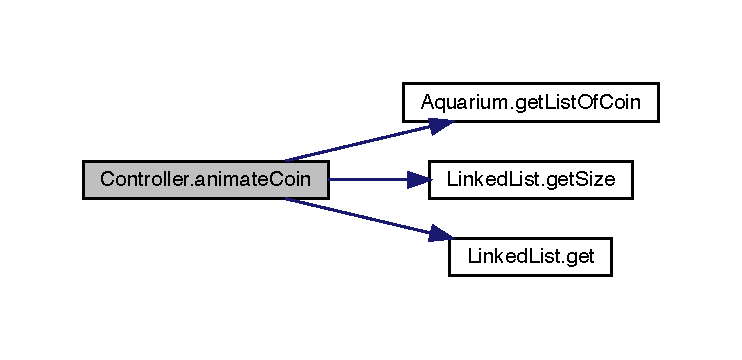
\includegraphics[width=350pt]{class_controller_a2996989c163af44339ea43f597b77115_cgraph}
\end{center}
\end{figure}
\mbox{\Hypertarget{class_controller_a04e239635c1b5ca996b74498c373626b}\label{class_controller_a04e239635c1b5ca996b74498c373626b}} 
\index{Controller@{Controller}!animate\+Egg@{animate\+Egg}}
\index{animate\+Egg@{animate\+Egg}!Controller@{Controller}}
\subsubsection{\texorpdfstring{animate\+Egg()}{animateEgg()}}
{\footnotesize\ttfamily void Controller.\+animate\+Egg (\begin{DoxyParamCaption}\item[{Graphics}]{g,  }\item[{Toolkit}]{t }\end{DoxyParamCaption})\hspace{0.3cm}{\ttfamily [inline]}}

animate egg. 
\begin{DoxyParams}{Parameters}
{\em g} & graphic. \\
\hline
{\em t} & toolkit. \\
\hline
\end{DoxyParams}
Here is the call graph for this function\+:
\nopagebreak
\begin{figure}[H]
\begin{center}
\leavevmode
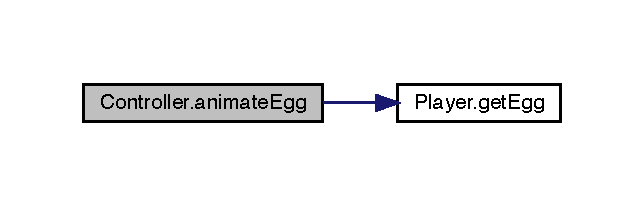
\includegraphics[width=309pt]{class_controller_a04e239635c1b5ca996b74498c373626b_cgraph}
\end{center}
\end{figure}
\mbox{\Hypertarget{class_controller_ac9f6dcbe9113ca383adf751261c2a8d3}\label{class_controller_ac9f6dcbe9113ca383adf751261c2a8d3}} 
\index{Controller@{Controller}!animate\+Fish\+Food@{animate\+Fish\+Food}}
\index{animate\+Fish\+Food@{animate\+Fish\+Food}!Controller@{Controller}}
\subsubsection{\texorpdfstring{animate\+Fish\+Food()}{animateFishFood()}}
{\footnotesize\ttfamily void Controller.\+animate\+Fish\+Food (\begin{DoxyParamCaption}{ }\end{DoxyParamCaption})\hspace{0.3cm}{\ttfamily [inline]}}

animate \mbox{\hyperlink{class_fish_food}{Fish\+Food}}. Here is the call graph for this function\+:
\nopagebreak
\begin{figure}[H]
\begin{center}
\leavevmode
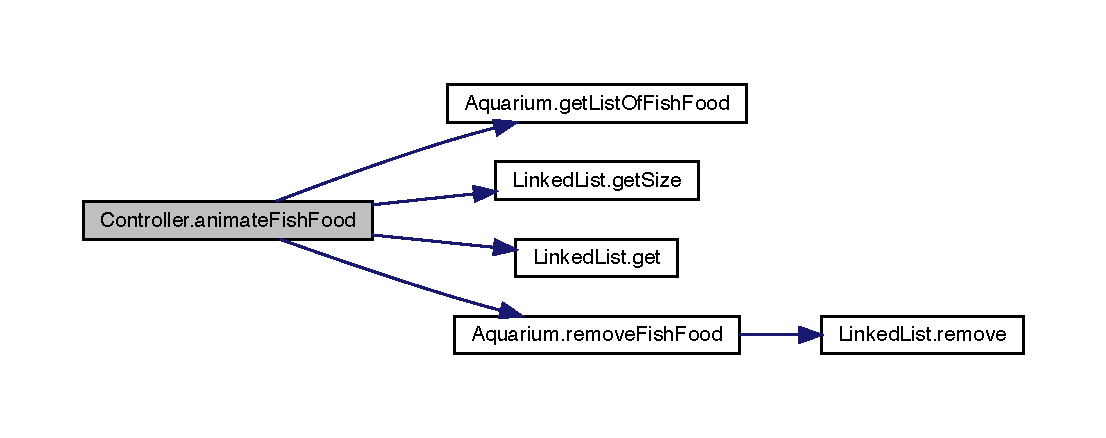
\includegraphics[width=350pt]{class_controller_ac9f6dcbe9113ca383adf751261c2a8d3_cgraph}
\end{center}
\end{figure}
\mbox{\Hypertarget{class_controller_ac950a5d811e4f3d266e8952e0140faa0}\label{class_controller_ac950a5d811e4f3d266e8952e0140faa0}} 
\index{Controller@{Controller}!animate\+Guppy@{animate\+Guppy}}
\index{animate\+Guppy@{animate\+Guppy}!Controller@{Controller}}
\subsubsection{\texorpdfstring{animate\+Guppy()}{animateGuppy()}}
{\footnotesize\ttfamily void Controller.\+animate\+Guppy (\begin{DoxyParamCaption}{ }\end{DoxyParamCaption})\hspace{0.3cm}{\ttfamily [inline]}}

animate guppy. Here is the call graph for this function\+:
\nopagebreak
\begin{figure}[H]
\begin{center}
\leavevmode
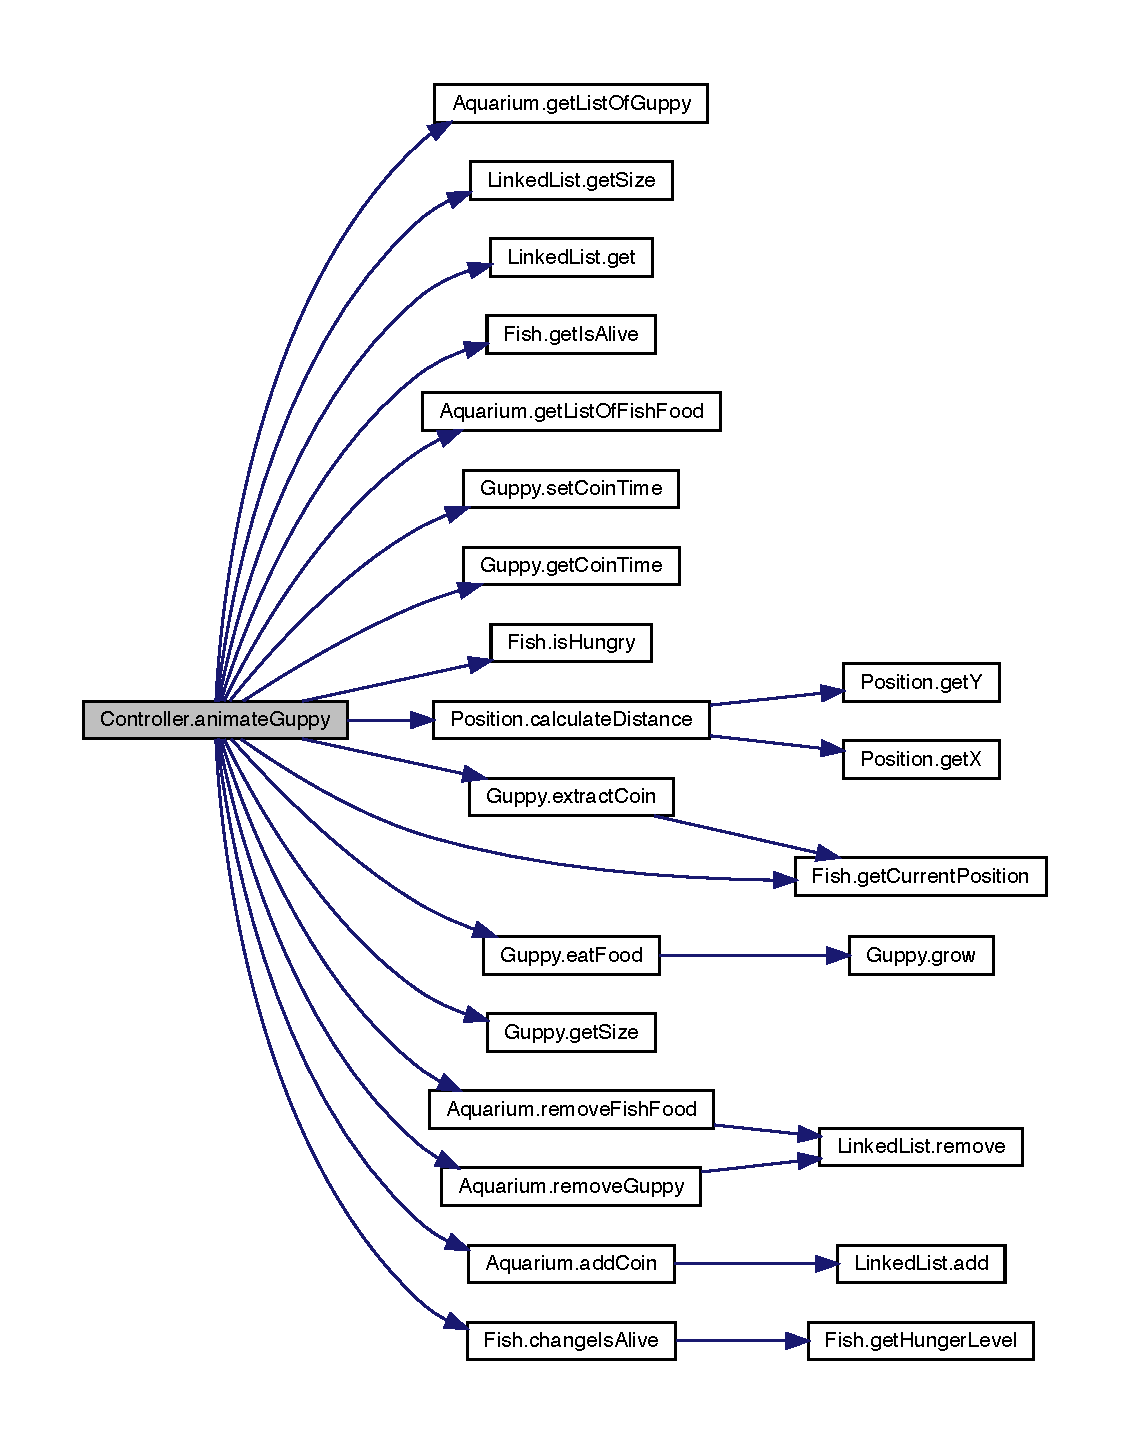
\includegraphics[width=350pt]{class_controller_ac950a5d811e4f3d266e8952e0140faa0_cgraph}
\end{center}
\end{figure}
\mbox{\Hypertarget{class_controller_a4a6a2af6faf89e4bc96bac2dc8b190f4}\label{class_controller_a4a6a2af6faf89e4bc96bac2dc8b190f4}} 
\index{Controller@{Controller}!animate\+Piranha@{animate\+Piranha}}
\index{animate\+Piranha@{animate\+Piranha}!Controller@{Controller}}
\subsubsection{\texorpdfstring{animate\+Piranha()}{animatePiranha()}}
{\footnotesize\ttfamily void Controller.\+animate\+Piranha (\begin{DoxyParamCaption}{ }\end{DoxyParamCaption})\hspace{0.3cm}{\ttfamily [inline]}}

animate piranha. Here is the call graph for this function\+:
\nopagebreak
\begin{figure}[H]
\begin{center}
\leavevmode
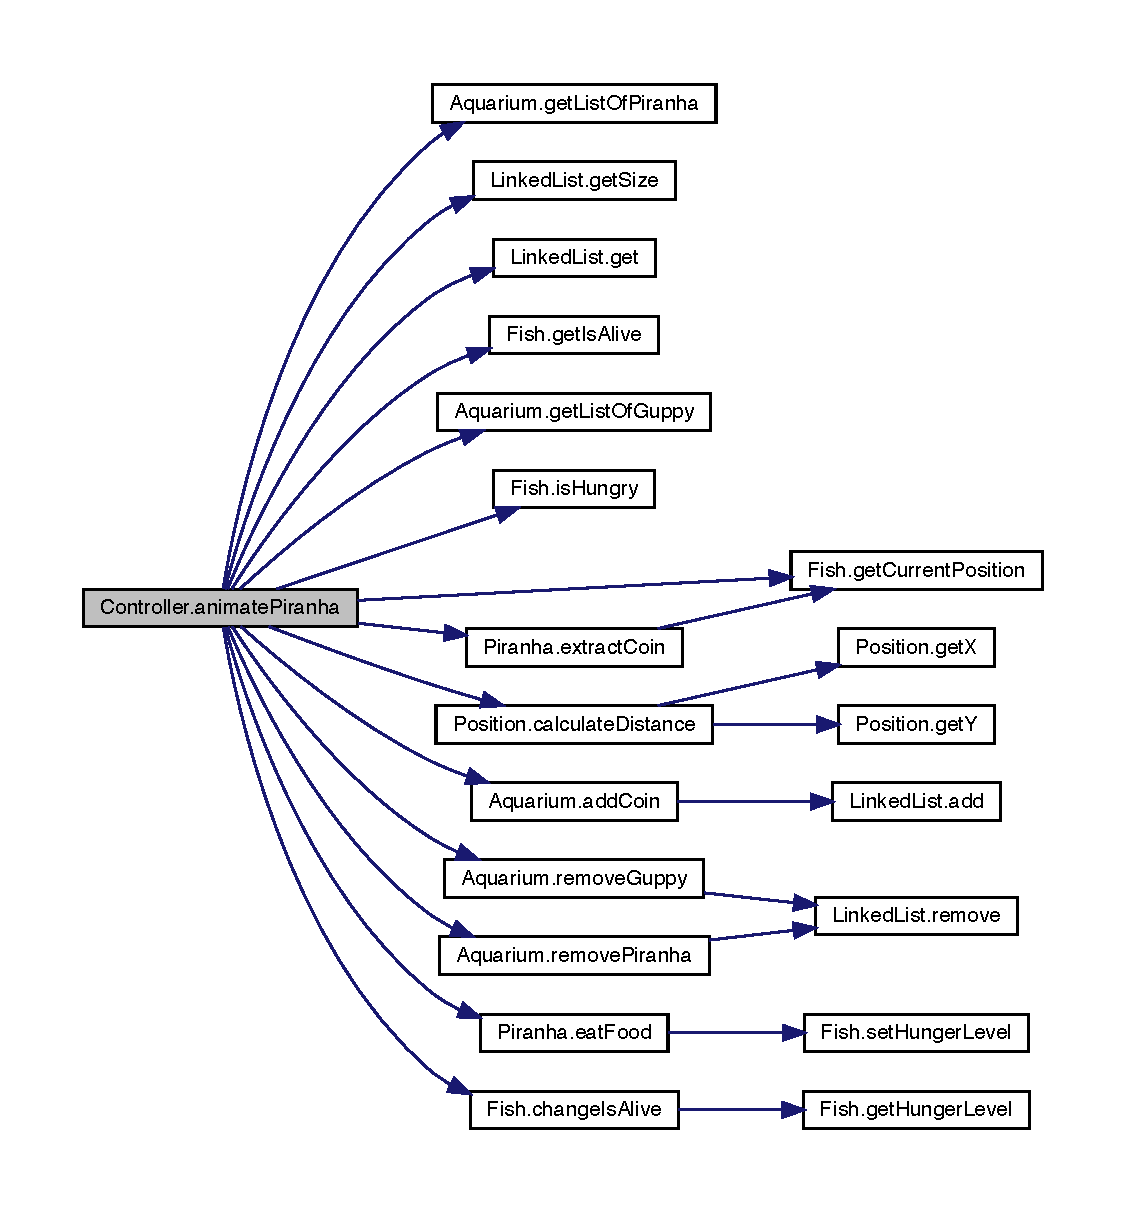
\includegraphics[width=350pt]{class_controller_a4a6a2af6faf89e4bc96bac2dc8b190f4_cgraph}
\end{center}
\end{figure}
\mbox{\Hypertarget{class_controller_a76a0629c8b8af69dfbf0cead4e6d04c3}\label{class_controller_a76a0629c8b8af69dfbf0cead4e6d04c3}} 
\index{Controller@{Controller}!animate\+Snail@{animate\+Snail}}
\index{animate\+Snail@{animate\+Snail}!Controller@{Controller}}
\subsubsection{\texorpdfstring{animate\+Snail()}{animateSnail()}}
{\footnotesize\ttfamily void Controller.\+animate\+Snail (\begin{DoxyParamCaption}{ }\end{DoxyParamCaption})\hspace{0.3cm}{\ttfamily [inline]}}

animate \mbox{\hyperlink{class_snail}{Snail}}. Here is the call graph for this function\+:
\nopagebreak
\begin{figure}[H]
\begin{center}
\leavevmode
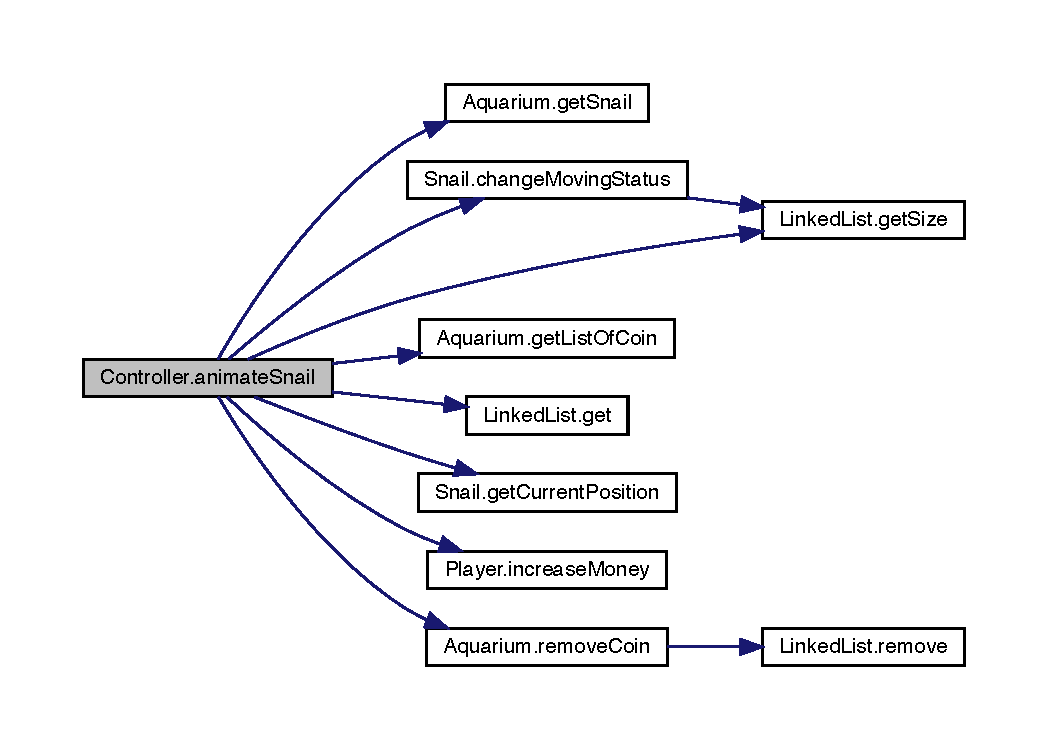
\includegraphics[width=350pt]{class_controller_a76a0629c8b8af69dfbf0cead4e6d04c3_cgraph}
\end{center}
\end{figure}
\mbox{\Hypertarget{class_controller_a278f0ba8f8978834619465f1eb357175}\label{class_controller_a278f0ba8f8978834619465f1eb357175}} 
\index{Controller@{Controller}!buy\+Egg@{buy\+Egg}}
\index{buy\+Egg@{buy\+Egg}!Controller@{Controller}}
\subsubsection{\texorpdfstring{buy\+Egg()}{buyEgg()}}
{\footnotesize\ttfamily void Controller.\+buy\+Egg (\begin{DoxyParamCaption}{ }\end{DoxyParamCaption})\hspace{0.3cm}{\ttfamily [inline]}}

buy egg. Here is the call graph for this function\+:
\nopagebreak
\begin{figure}[H]
\begin{center}
\leavevmode
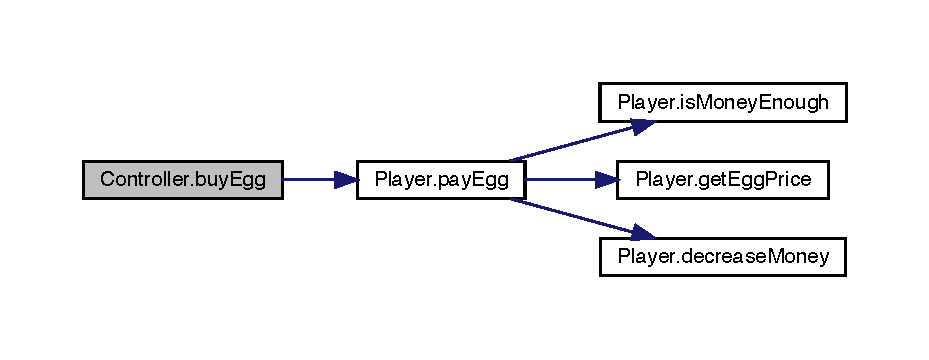
\includegraphics[width=350pt]{class_controller_a278f0ba8f8978834619465f1eb357175_cgraph}
\end{center}
\end{figure}
\mbox{\Hypertarget{class_controller_a40a60157abffab52f9170ffb6579151e}\label{class_controller_a40a60157abffab52f9170ffb6579151e}} 
\index{Controller@{Controller}!buy\+Food@{buy\+Food}}
\index{buy\+Food@{buy\+Food}!Controller@{Controller}}
\subsubsection{\texorpdfstring{buy\+Food()}{buyFood()}}
{\footnotesize\ttfamily void Controller.\+buy\+Food (\begin{DoxyParamCaption}\item[{\mbox{\hyperlink{class_position}{Position}}}]{init\+Position }\end{DoxyParamCaption})\hspace{0.3cm}{\ttfamily [inline]}}

buy food. 
\begin{DoxyParams}{Parameters}
{\em init\+Position} & object \mbox{\hyperlink{class_position}{Position}} of the food. \\
\hline
\end{DoxyParams}
Here is the call graph for this function\+:
\nopagebreak
\begin{figure}[H]
\begin{center}
\leavevmode
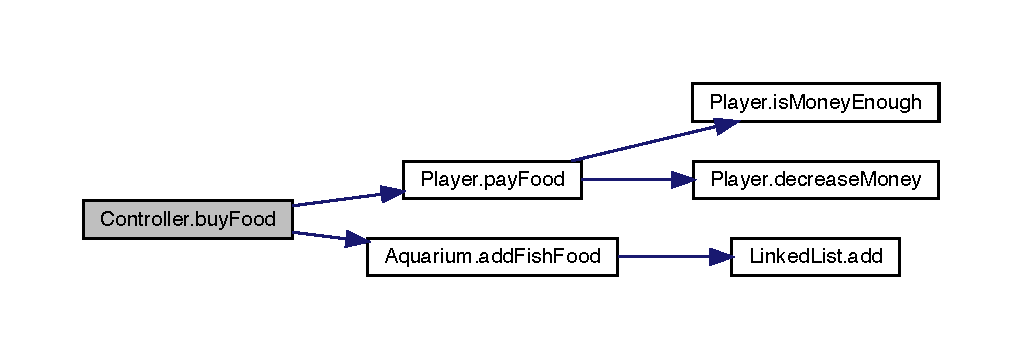
\includegraphics[width=350pt]{class_controller_a40a60157abffab52f9170ffb6579151e_cgraph}
\end{center}
\end{figure}
\mbox{\Hypertarget{class_controller_adb93f92dca6e1d48d61d811411945aff}\label{class_controller_adb93f92dca6e1d48d61d811411945aff}} 
\index{Controller@{Controller}!buy\+Guppy@{buy\+Guppy}}
\index{buy\+Guppy@{buy\+Guppy}!Controller@{Controller}}
\subsubsection{\texorpdfstring{buy\+Guppy()}{buyGuppy()}}
{\footnotesize\ttfamily void Controller.\+buy\+Guppy (\begin{DoxyParamCaption}{ }\end{DoxyParamCaption})\hspace{0.3cm}{\ttfamily [inline]}}

buy guppy. Here is the call graph for this function\+:
\nopagebreak
\begin{figure}[H]
\begin{center}
\leavevmode
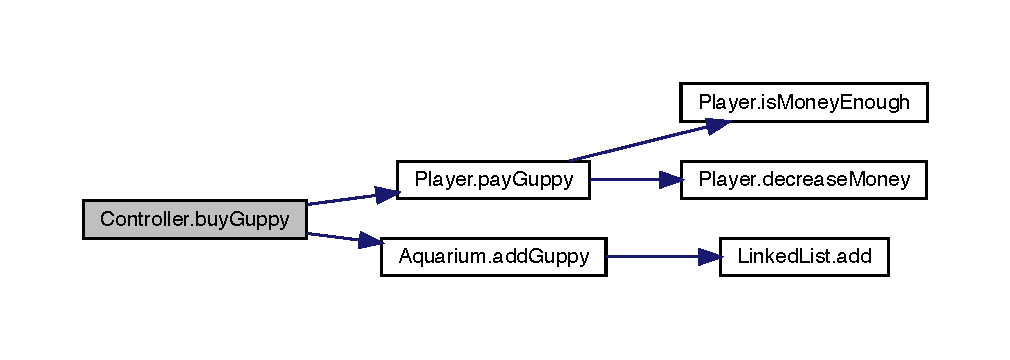
\includegraphics[width=350pt]{class_controller_adb93f92dca6e1d48d61d811411945aff_cgraph}
\end{center}
\end{figure}
\mbox{\Hypertarget{class_controller_aeea16d5cb5dc9ea882583b621c1205f9}\label{class_controller_aeea16d5cb5dc9ea882583b621c1205f9}} 
\index{Controller@{Controller}!buy\+Piranha@{buy\+Piranha}}
\index{buy\+Piranha@{buy\+Piranha}!Controller@{Controller}}
\subsubsection{\texorpdfstring{buy\+Piranha()}{buyPiranha()}}
{\footnotesize\ttfamily void Controller.\+buy\+Piranha (\begin{DoxyParamCaption}{ }\end{DoxyParamCaption})\hspace{0.3cm}{\ttfamily [inline]}}

buy piranha. Here is the call graph for this function\+:
\nopagebreak
\begin{figure}[H]
\begin{center}
\leavevmode
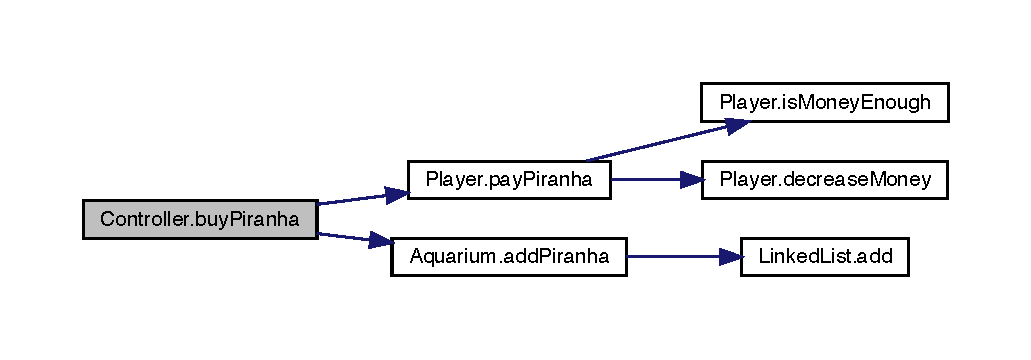
\includegraphics[width=350pt]{class_controller_aeea16d5cb5dc9ea882583b621c1205f9_cgraph}
\end{center}
\end{figure}
\mbox{\Hypertarget{class_controller_afcc995c6e49e732f0542a4dee21921d2}\label{class_controller_afcc995c6e49e732f0542a4dee21921d2}} 
\index{Controller@{Controller}!draw\+And\+Animate\+Object@{draw\+And\+Animate\+Object}}
\index{draw\+And\+Animate\+Object@{draw\+And\+Animate\+Object}!Controller@{Controller}}
\subsubsection{\texorpdfstring{draw\+And\+Animate\+Object()}{drawAndAnimateObject()}}
{\footnotesize\ttfamily void Controller.\+draw\+And\+Animate\+Object (\begin{DoxyParamCaption}\item[{Graphics}]{g,  }\item[{Toolkit}]{t }\end{DoxyParamCaption})\hspace{0.3cm}{\ttfamily [inline]}}

Generic method to draw and animate every object in aquarium. 
\begin{DoxyParams}{Parameters}
{\em g} & graphic. \\
\hline
{\em t} & Toolkit. \\
\hline
\end{DoxyParams}
Here is the call graph for this function\+:
\nopagebreak
\begin{figure}[H]
\begin{center}
\leavevmode
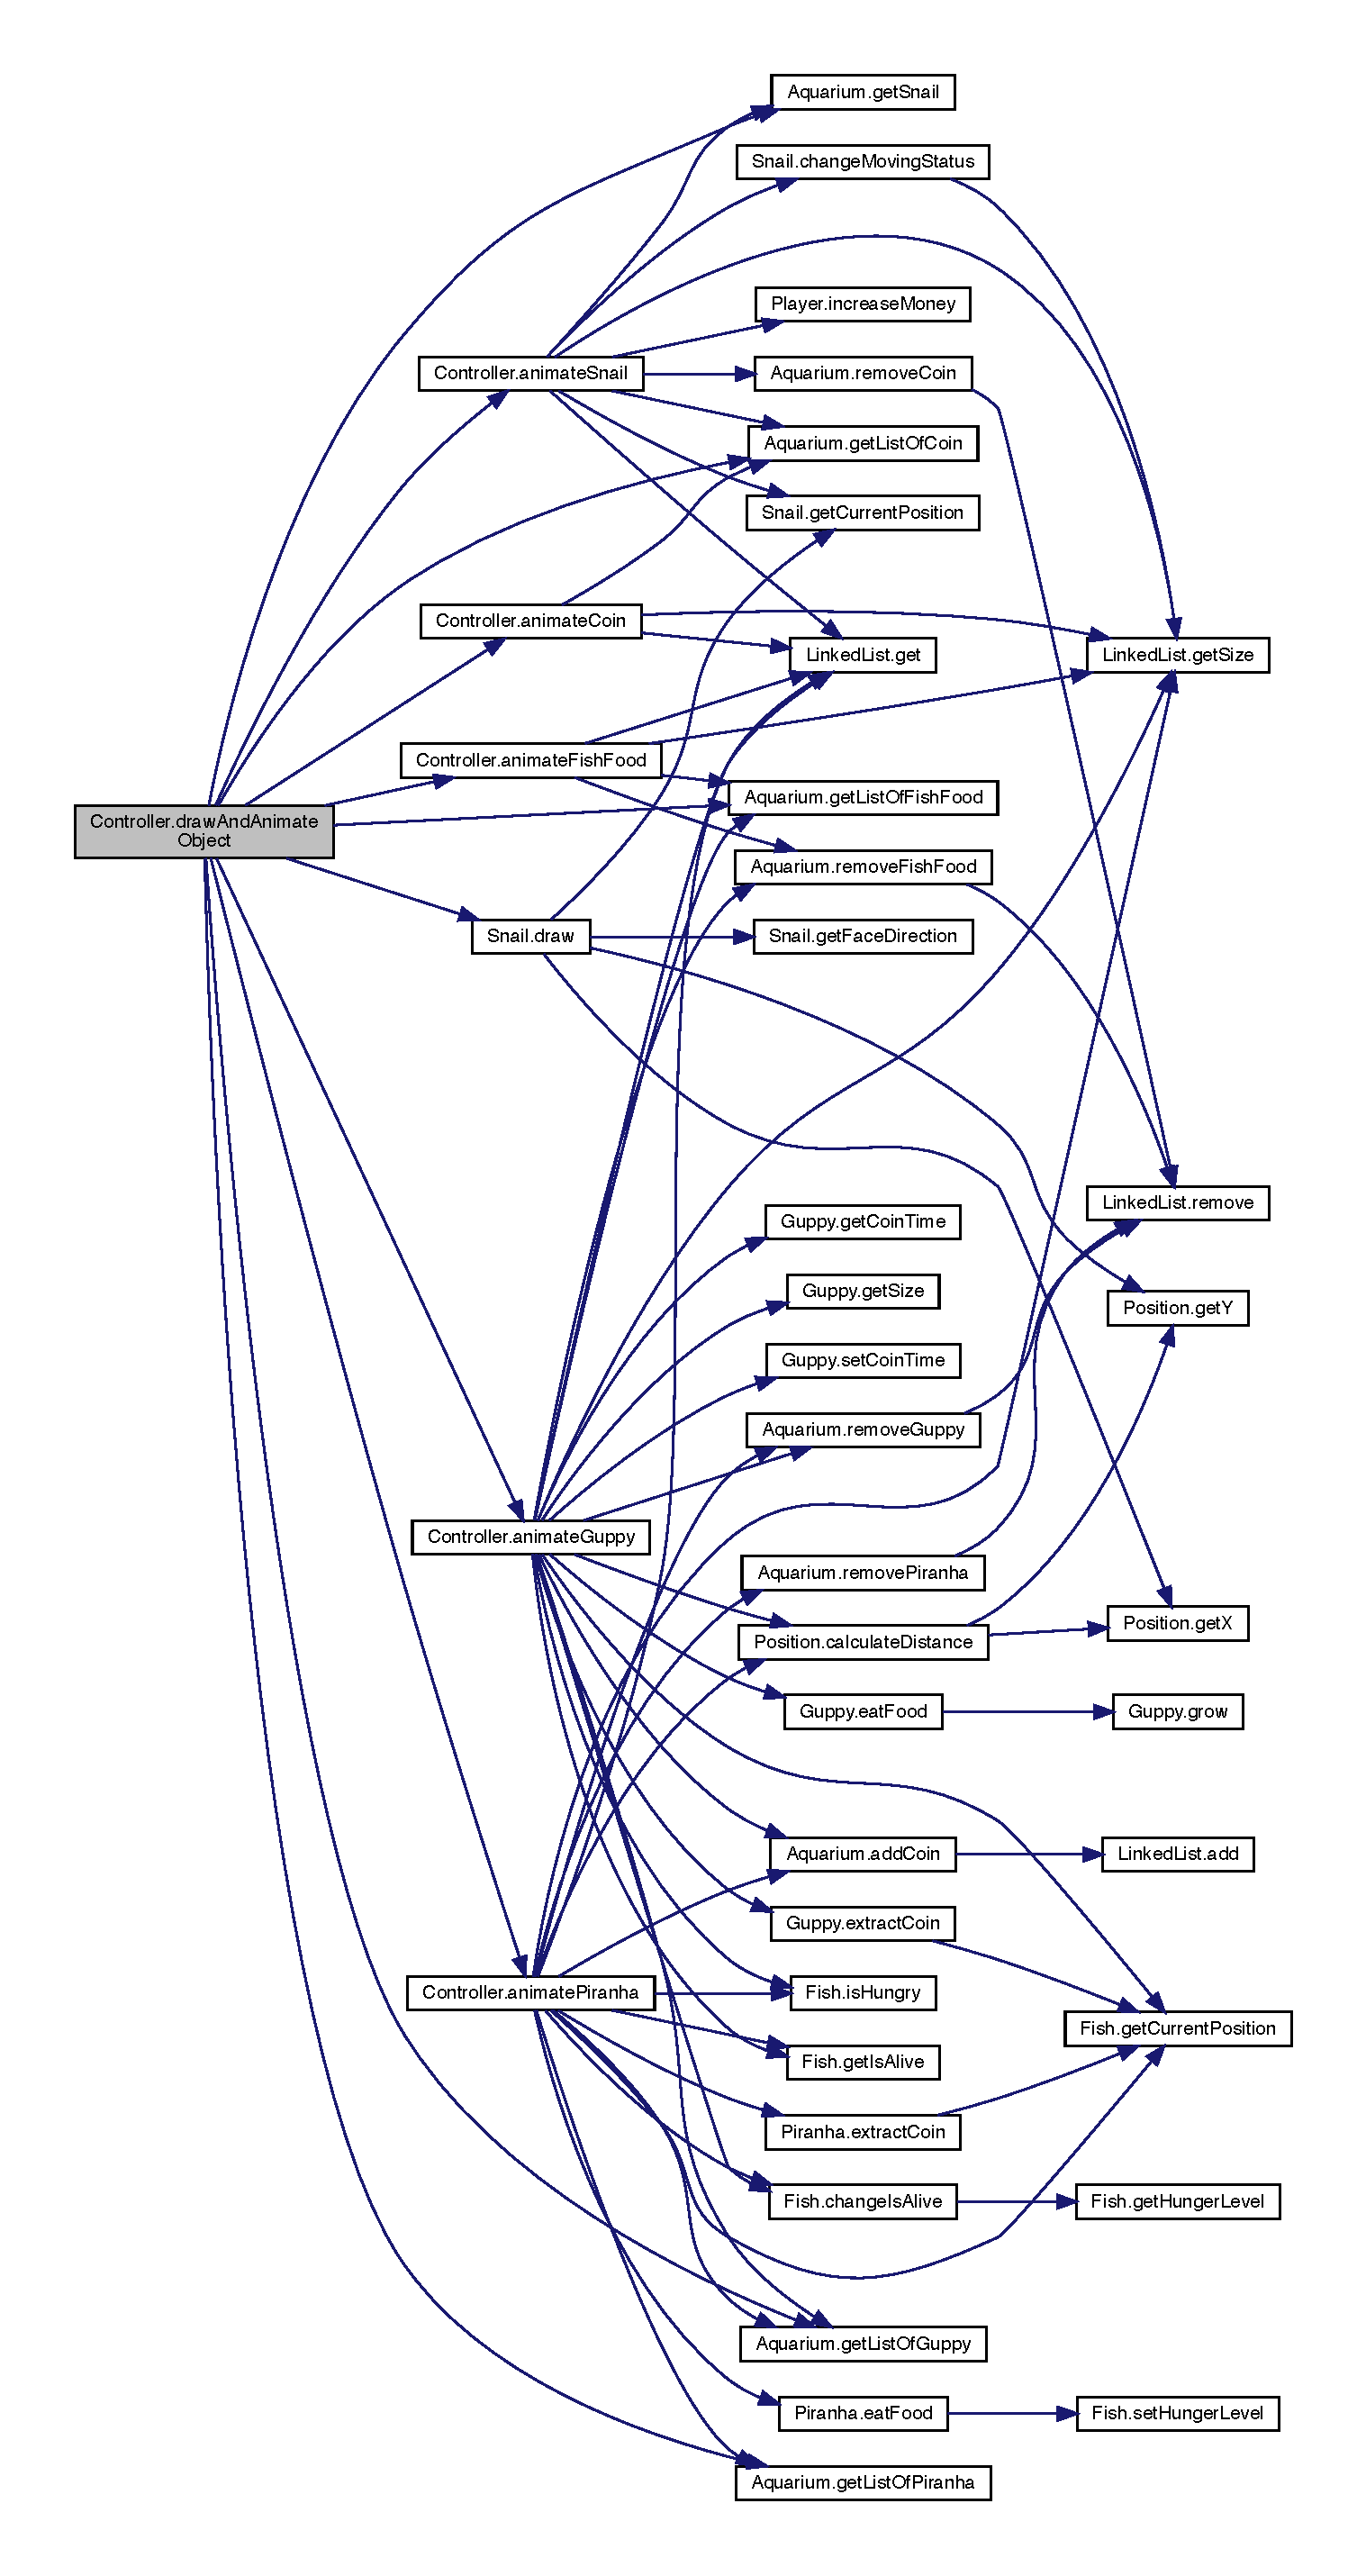
\includegraphics[height=550pt]{class_controller_afcc995c6e49e732f0542a4dee21921d2_cgraph}
\end{center}
\end{figure}
\mbox{\Hypertarget{class_controller_a42fbd01fdeefdf2f40f85230f40d8be8}\label{class_controller_a42fbd01fdeefdf2f40f85230f40d8be8}} 
\index{Controller@{Controller}!get\+Coin@{get\+Coin}}
\index{get\+Coin@{get\+Coin}!Controller@{Controller}}
\subsubsection{\texorpdfstring{get\+Coin()}{getCoin()}}
{\footnotesize\ttfamily boolean Controller.\+get\+Coin (\begin{DoxyParamCaption}\item[{Mouse\+Event}]{e }\end{DoxyParamCaption})\hspace{0.3cm}{\ttfamily [inline]}}

get\+Coin using mouse event. 
\begin{DoxyParams}{Parameters}
{\em e} & Mouseevent. \\
\hline
\end{DoxyParams}
\begin{DoxyReturn}{Returns}
get\+Coin boolean. 
\end{DoxyReturn}
Here is the call graph for this function\+:
\nopagebreak
\begin{figure}[H]
\begin{center}
\leavevmode
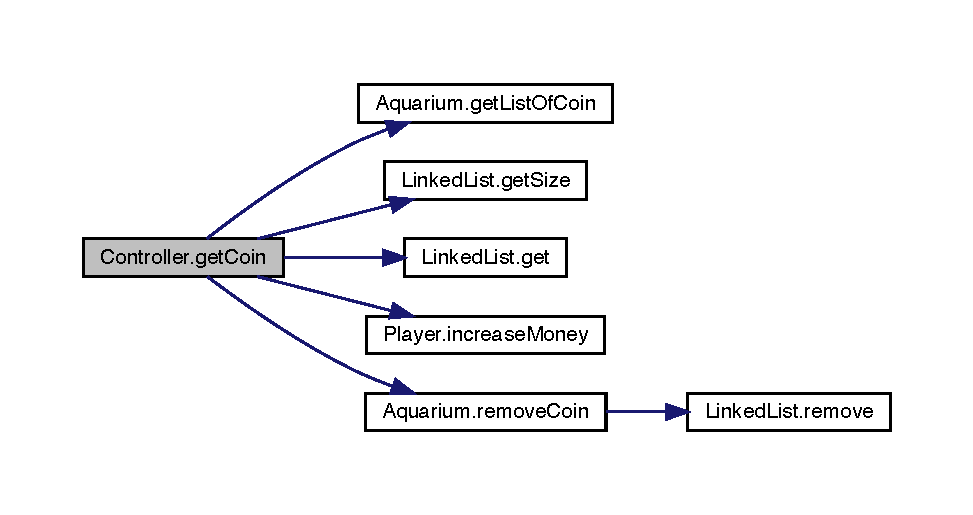
\includegraphics[width=350pt]{class_controller_a42fbd01fdeefdf2f40f85230f40d8be8_cgraph}
\end{center}
\end{figure}
\mbox{\Hypertarget{class_controller_af6b9d4cd41e5bb90f04c0f61f5cfcd2d}\label{class_controller_af6b9d4cd41e5bb90f04c0f61f5cfcd2d}} 
\index{Controller@{Controller}!graphic\+Accesories@{graphic\+Accesories}}
\index{graphic\+Accesories@{graphic\+Accesories}!Controller@{Controller}}
\subsubsection{\texorpdfstring{graphic\+Accesories()}{graphicAccesories()}}
{\footnotesize\ttfamily void Controller.\+graphic\+Accesories (\begin{DoxyParamCaption}\item[{Graphics}]{g,  }\item[{Toolkit}]{t }\end{DoxyParamCaption})\hspace{0.3cm}{\ttfamily [inline]}}

draw text and sprite needed for the game. 
\begin{DoxyParams}{Parameters}
{\em g} & graphic. \\
\hline
{\em t} & toolkit. \\
\hline
\end{DoxyParams}
Here is the call graph for this function\+:
\nopagebreak
\begin{figure}[H]
\begin{center}
\leavevmode
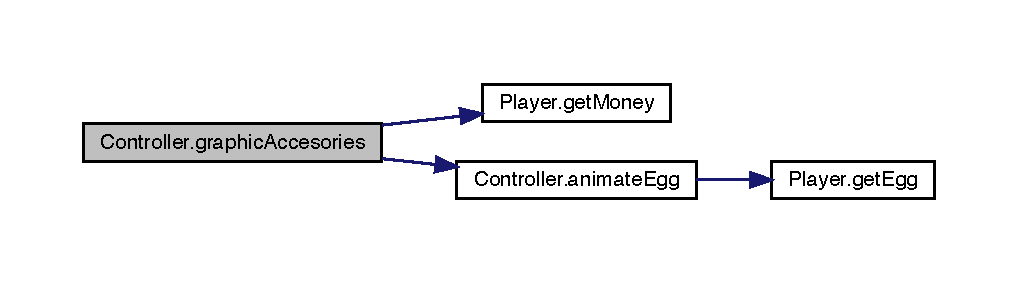
\includegraphics[width=350pt]{class_controller_af6b9d4cd41e5bb90f04c0f61f5cfcd2d_cgraph}
\end{center}
\end{figure}
\mbox{\Hypertarget{class_controller_a3d48c05f5876d46347a4b22f3d6d5a1a}\label{class_controller_a3d48c05f5876d46347a4b22f3d6d5a1a}} 
\index{Controller@{Controller}!paint\+Component@{paint\+Component}}
\index{paint\+Component@{paint\+Component}!Controller@{Controller}}
\subsubsection{\texorpdfstring{paint\+Component()}{paintComponent()}}
{\footnotesize\ttfamily void Controller.\+paint\+Component (\begin{DoxyParamCaption}\item[{Graphics}]{g }\end{DoxyParamCaption})\hspace{0.3cm}{\ttfamily [inline]}}

paint. 
\begin{DoxyParams}{Parameters}
{\em g} & graphic. \\
\hline
\end{DoxyParams}
Here is the call graph for this function\+:
\nopagebreak
\begin{figure}[H]
\begin{center}
\leavevmode
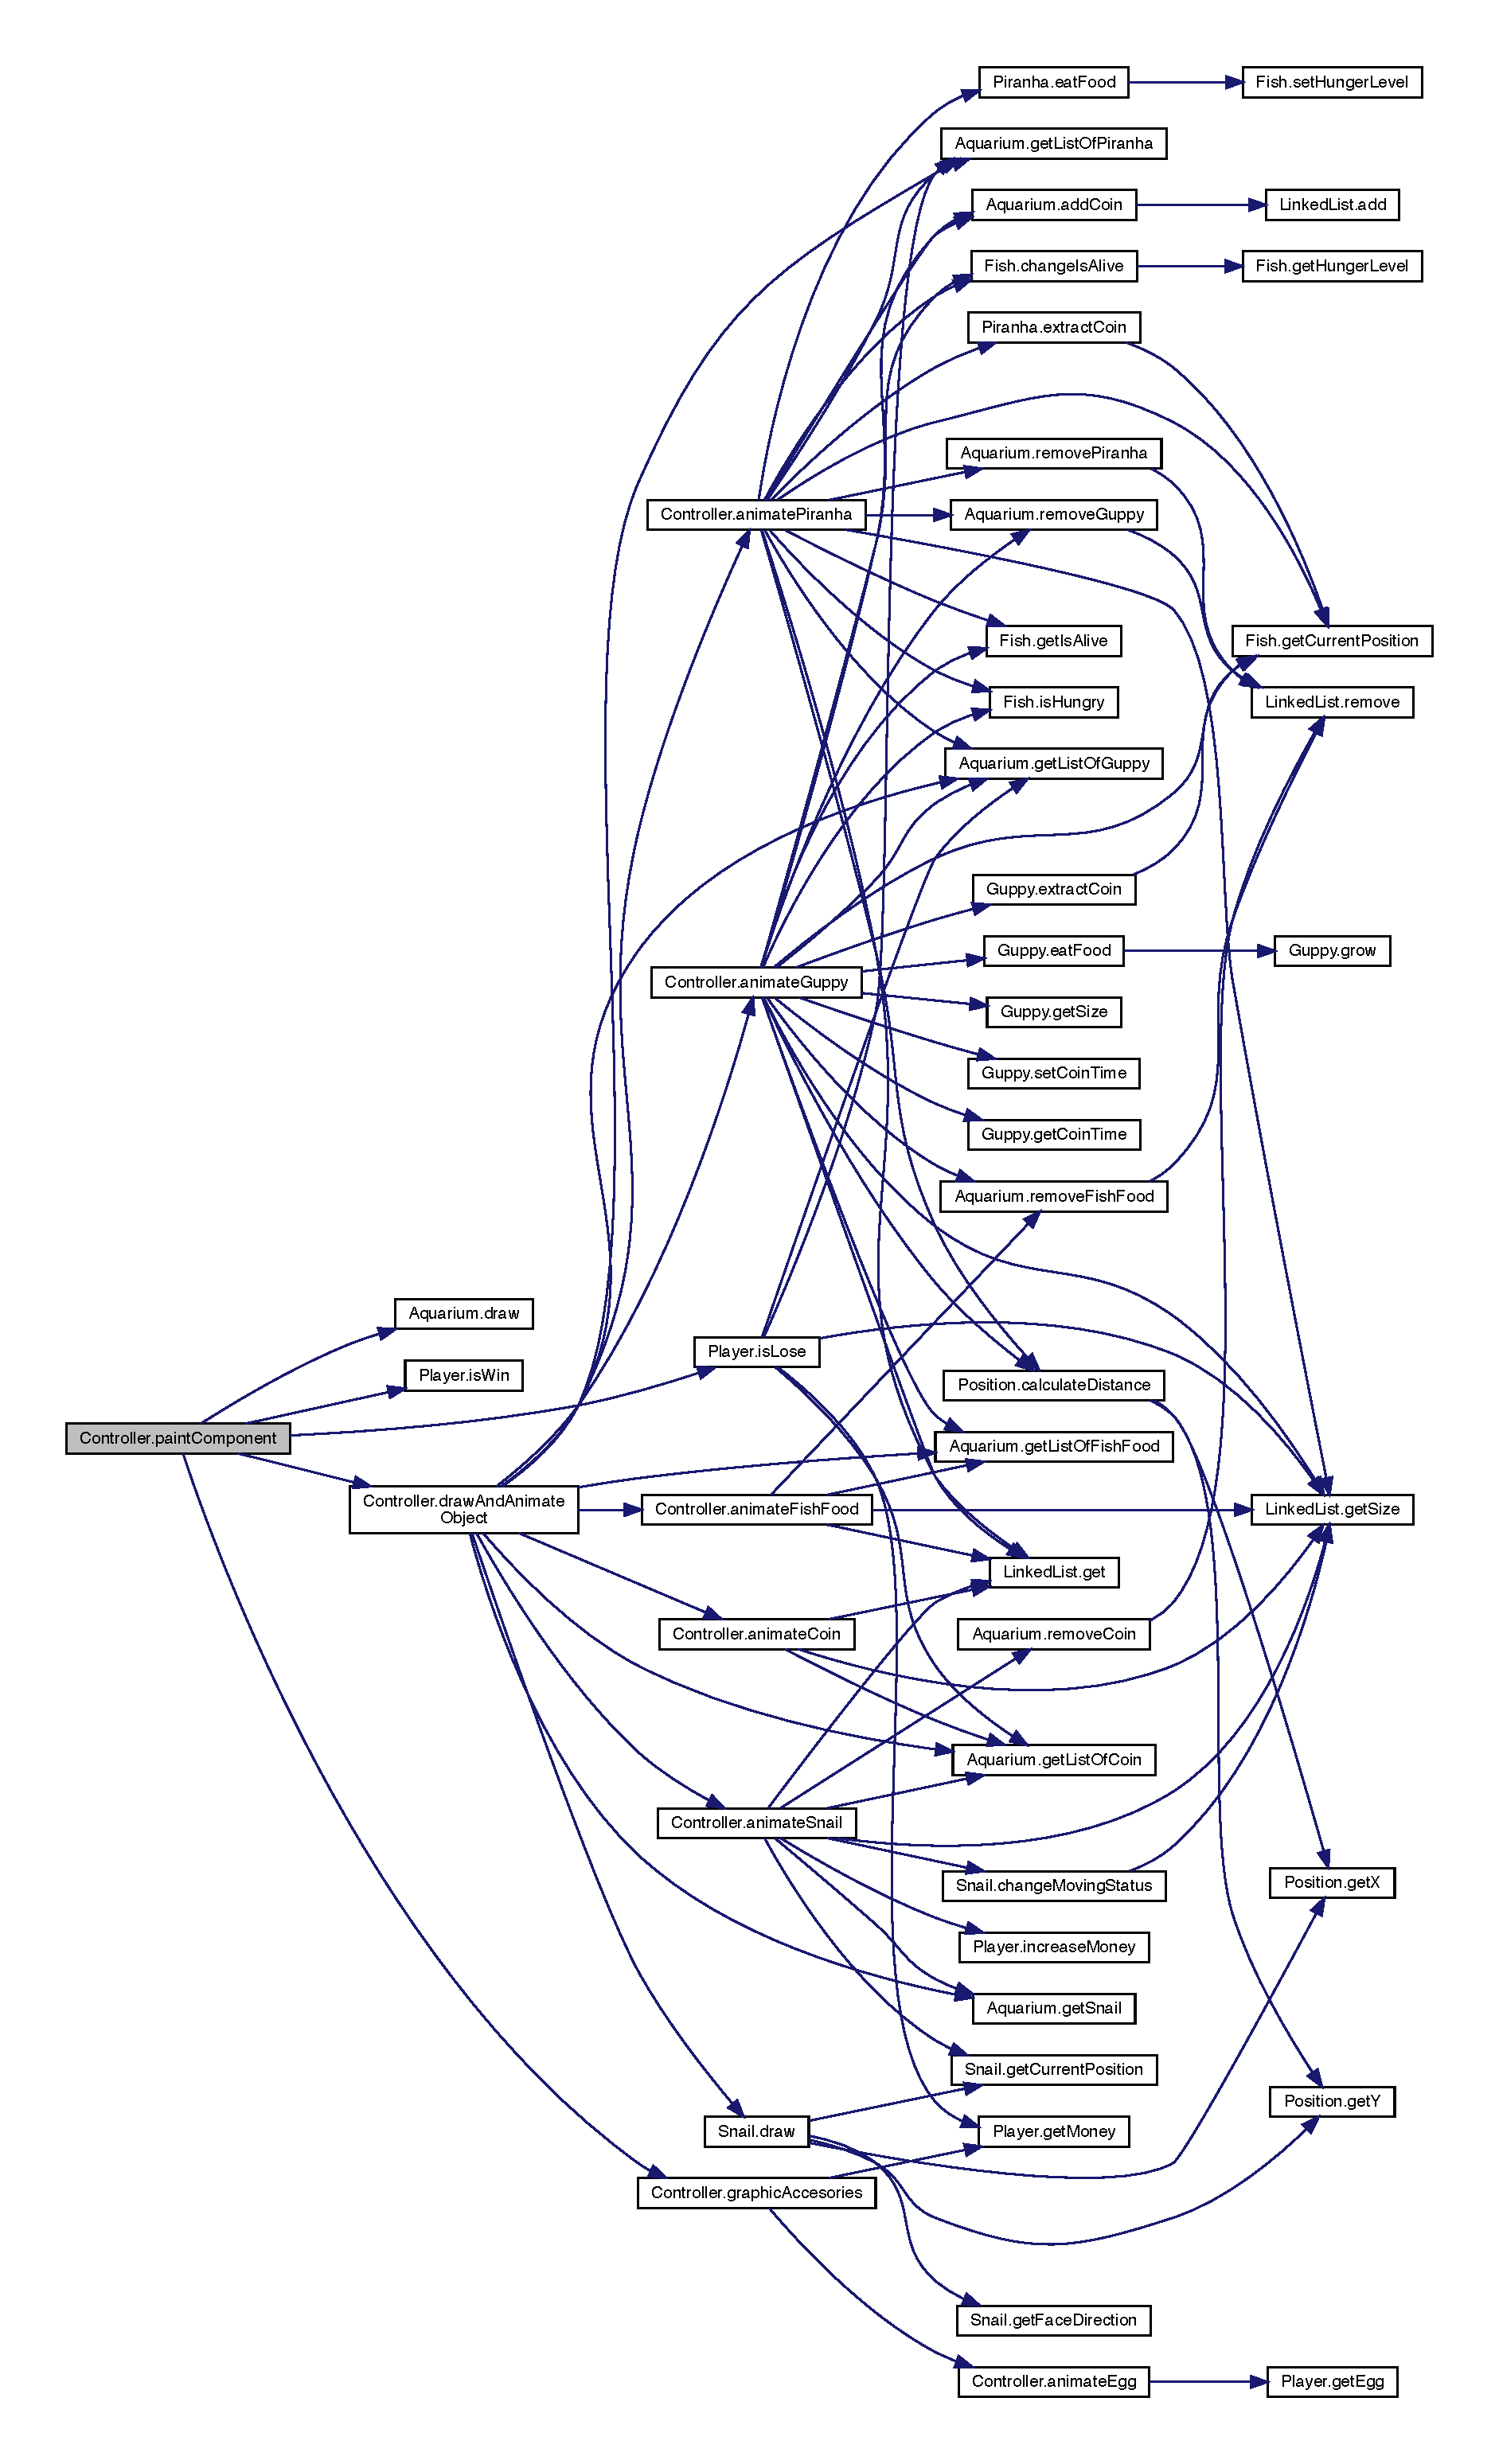
\includegraphics[height=550pt]{class_controller_a3d48c05f5876d46347a4b22f3d6d5a1a_cgraph}
\end{center}
\end{figure}
\mbox{\Hypertarget{class_controller_a2fcfd8c4d229d4deeec470de95567805}\label{class_controller_a2fcfd8c4d229d4deeec470de95567805}} 
\index{Controller@{Controller}!run@{run}}
\index{run@{run}!Controller@{Controller}}
\subsubsection{\texorpdfstring{run()}{run()}}
{\footnotesize\ttfamily void Controller.\+run (\begin{DoxyParamCaption}{ }\end{DoxyParamCaption})\hspace{0.3cm}{\ttfamily [inline]}}

run. Here is the call graph for this function\+:
\nopagebreak
\begin{figure}[H]
\begin{center}
\leavevmode
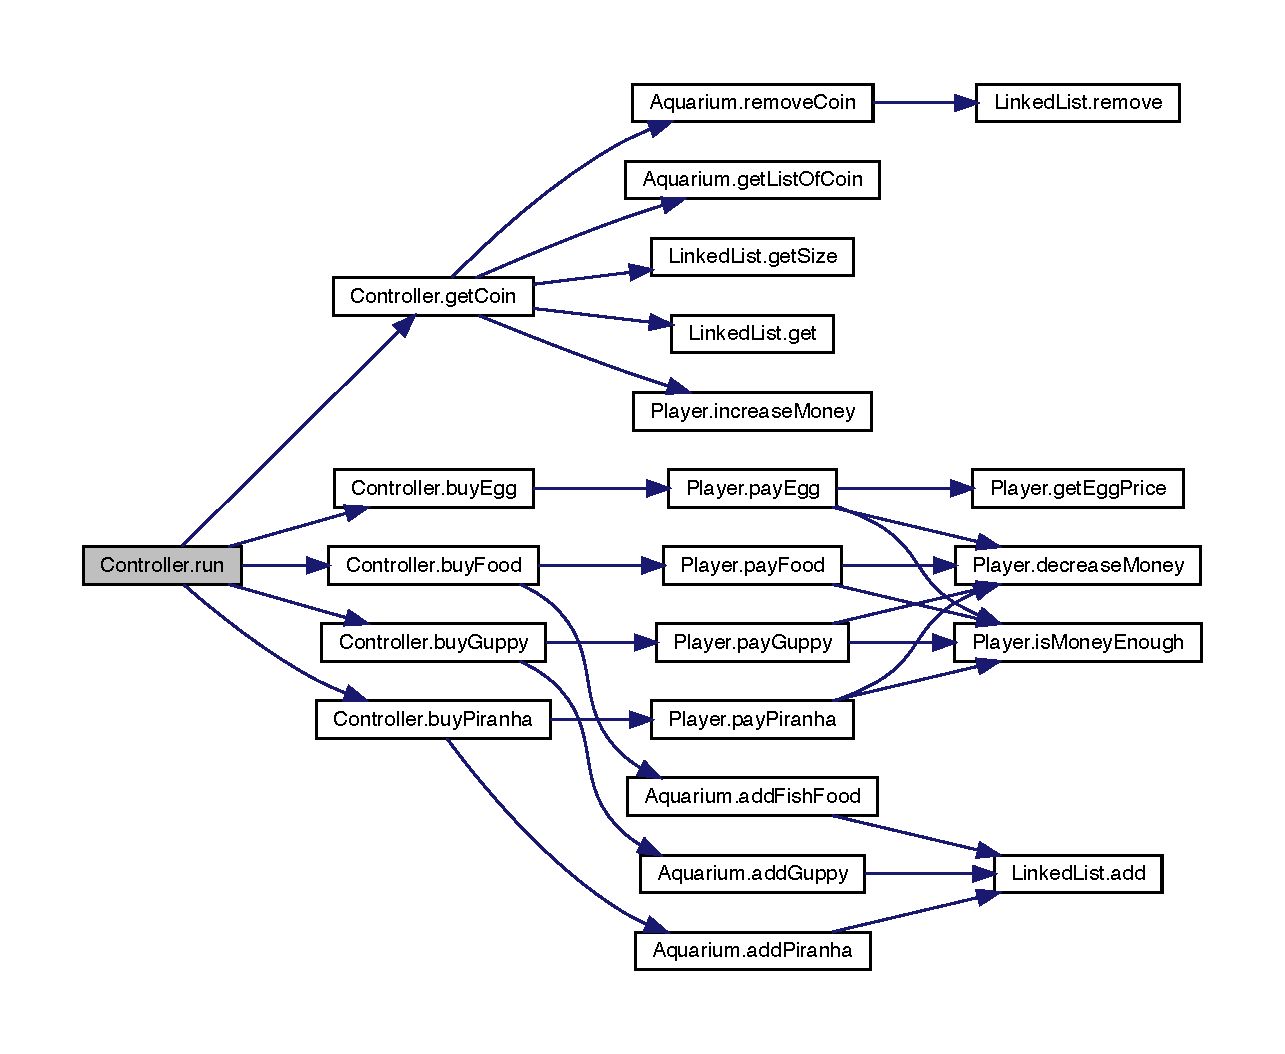
\includegraphics[width=350pt]{class_controller_a2fcfd8c4d229d4deeec470de95567805_cgraph}
\end{center}
\end{figure}


\subsection{Member Data Documentation}
\mbox{\Hypertarget{class_controller_a77eb7e2f012edbfa7296d765c3f11b52}\label{class_controller_a77eb7e2f012edbfa7296d765c3f11b52}} 
\index{Controller@{Controller}!f@{f}}
\index{f@{f}!Controller@{Controller}}
\subsubsection{\texorpdfstring{f}{f}}
{\footnotesize\ttfamily J\+Frame Controller.\+f = new J\+Frame(\char`\"{}Arkav\+Quarium\char`\"{})\hspace{0.3cm}{\ttfamily [static]}}

J\+Frame. \mbox{\Hypertarget{class_controller_a906f3cb8bda1e63ea53825652e155aaf}\label{class_controller_a906f3cb8bda1e63ea53825652e155aaf}} 
\index{Controller@{Controller}!player@{player}}
\index{player@{player}!Controller@{Controller}}
\subsubsection{\texorpdfstring{player}{player}}
{\footnotesize\ttfamily \mbox{\hyperlink{class_player}{Player}} Controller.\+player\hspace{0.3cm}{\ttfamily [private]}}

\mbox{\Hypertarget{class_controller_ad36875a9a542b89d92583d79567db811}\label{class_controller_ad36875a9a542b89d92583d79567db811}} 
\index{Controller@{Controller}!tank@{tank}}
\index{tank@{tank}!Controller@{Controller}}
\subsubsection{\texorpdfstring{tank}{tank}}
{\footnotesize\ttfamily \mbox{\hyperlink{class_aquarium}{Aquarium}} Controller.\+tank\hspace{0.3cm}{\ttfamily [private]}}

\mbox{\Hypertarget{class_controller_a2f43fd03a6aee6119a7d2d090555194b}\label{class_controller_a2f43fd03a6aee6119a7d2d090555194b}} 
\index{Controller@{Controller}!time@{time}}
\index{time@{time}!Controller@{Controller}}
\subsubsection{\texorpdfstring{time}{time}}
{\footnotesize\ttfamily Timer Controller.\+time\hspace{0.3cm}{\ttfamily [private]}}



The documentation for this class was generated from the following file\+:\begin{DoxyCompactItemize}
\item 
\mbox{\hyperlink{_controller_8java}{Controller.\+java}}\end{DoxyCompactItemize}

\hypertarget{interface_drawable}{}\section{Drawable Interface Reference}
\label{interface_drawable}\index{Drawable@{Drawable}}


Inheritance diagram for Drawable\+:
\nopagebreak
\begin{figure}[H]
\begin{center}
\leavevmode
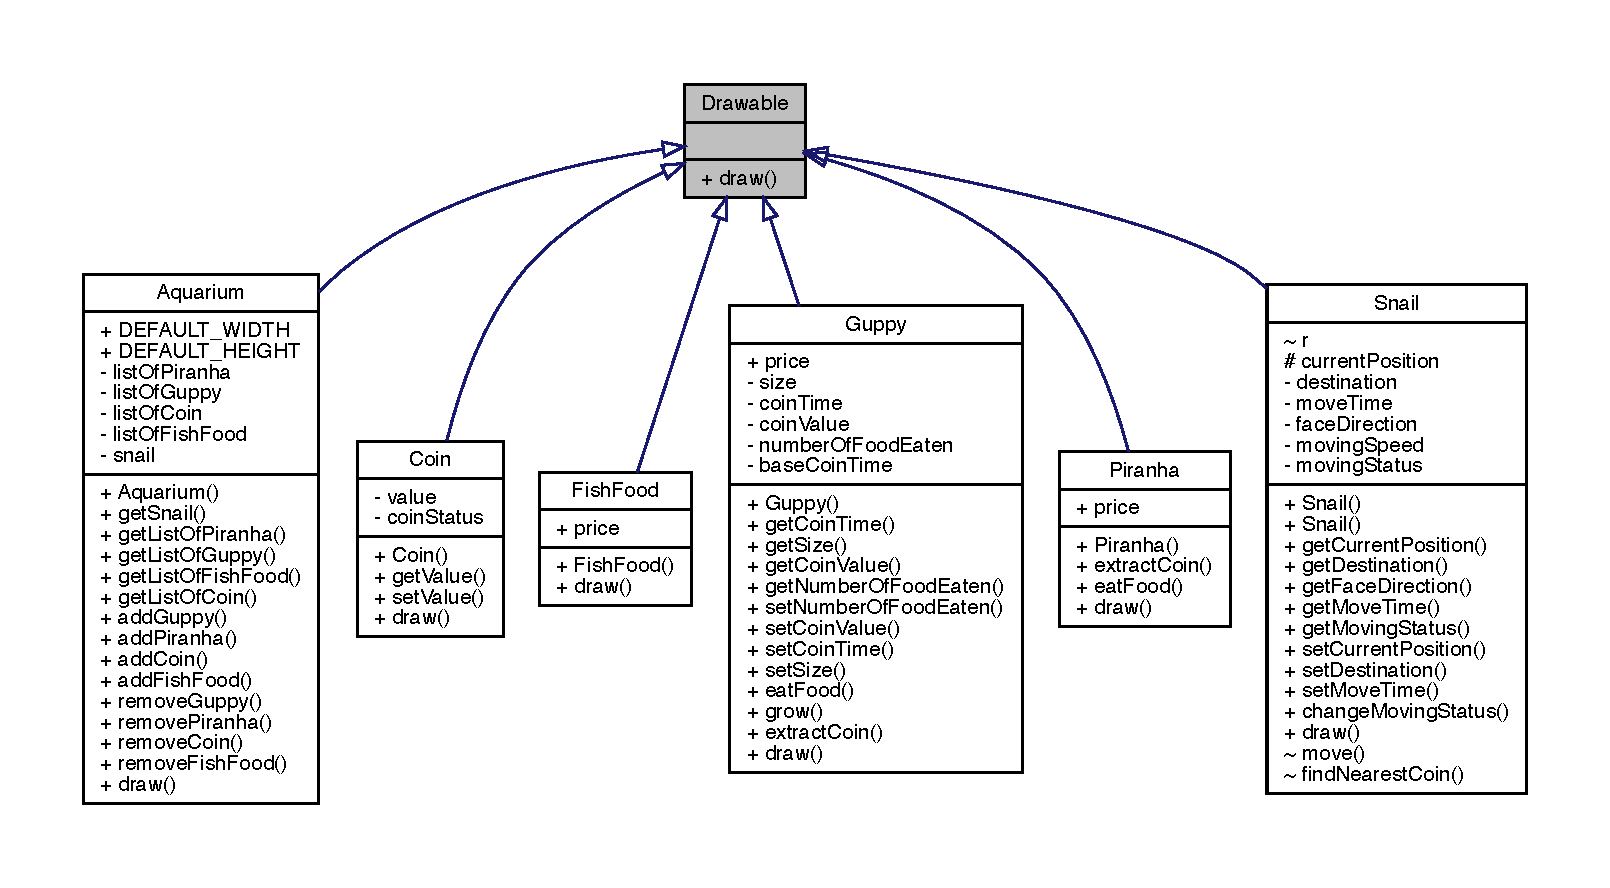
\includegraphics[width=350pt]{interface_drawable__inherit__graph}
\end{center}
\end{figure}


Collaboration diagram for Drawable\+:
\nopagebreak
\begin{figure}[H]
\begin{center}
\leavevmode
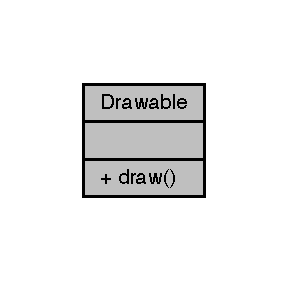
\includegraphics[width=138pt]{interface_drawable__coll__graph}
\end{center}
\end{figure}
\subsection*{Public Member Functions}
\begin{DoxyCompactItemize}
\item 
void \mbox{\hyperlink{interface_drawable_aaddafb212b3c8e60fcc742052570c893}{draw}} (Graphics g, Toolkit t)
\end{DoxyCompactItemize}


\subsection{Detailed Description}
Interface to draw object into visual representation. \begin{DoxyVersion}{Version}
1.\+0. 
\end{DoxyVersion}


\subsection{Member Function Documentation}
\mbox{\Hypertarget{interface_drawable_aaddafb212b3c8e60fcc742052570c893}\label{interface_drawable_aaddafb212b3c8e60fcc742052570c893}} 
\index{Drawable@{Drawable}!draw@{draw}}
\index{draw@{draw}!Drawable@{Drawable}}
\subsubsection{\texorpdfstring{draw()}{draw()}}
{\footnotesize\ttfamily void Drawable.\+draw (\begin{DoxyParamCaption}\item[{Graphics}]{g,  }\item[{Toolkit}]{t }\end{DoxyParamCaption})}

draw to aquarium. 
\begin{DoxyParams}{Parameters}
{\em g} & Draw container. \\
\hline
{\em t} & Object to grab image. \\
\hline
\end{DoxyParams}


Implemented in \mbox{\hyperlink{class_snail_aa39dc71c305e7034af0438f036232e43}{Snail}}, \mbox{\hyperlink{class_aquarium_af6a186c92c1f91f92ae382416b77d3c3}{Aquarium}}, \mbox{\hyperlink{class_guppy_ad04fab448adc11ff3eecf3a76c64781b}{Guppy}}, \mbox{\hyperlink{class_coin_ae0c35ffd80b39f26f43d287da0565d0b}{Coin}}, \mbox{\hyperlink{class_piranha_a8a06429a9c5b42fb4246f48c54d6cf78}{Piranha}}, and \mbox{\hyperlink{class_fish_food_a061d353336adc633607668e8d8a73b25}{Fish\+Food}}.



The documentation for this interface was generated from the following file\+:\begin{DoxyCompactItemize}
\item 
\mbox{\hyperlink{_drawable_8java}{Drawable.\+java}}\end{DoxyCompactItemize}

\hypertarget{class_droppable_item}{}\section{Droppable\+Item Class Reference}
\label{class_droppable_item}\index{Droppable\+Item@{Droppable\+Item}}


Inheritance diagram for Droppable\+Item\+:
\nopagebreak
\begin{figure}[H]
\begin{center}
\leavevmode
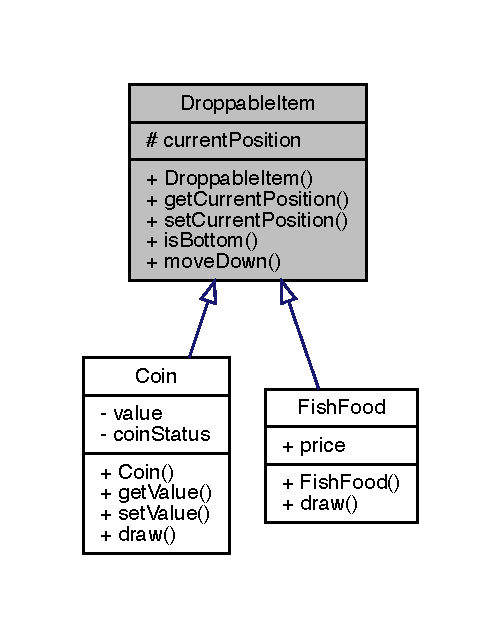
\includegraphics[width=240pt]{class_droppable_item__inherit__graph}
\end{center}
\end{figure}


Collaboration diagram for Droppable\+Item\+:
\nopagebreak
\begin{figure}[H]
\begin{center}
\leavevmode
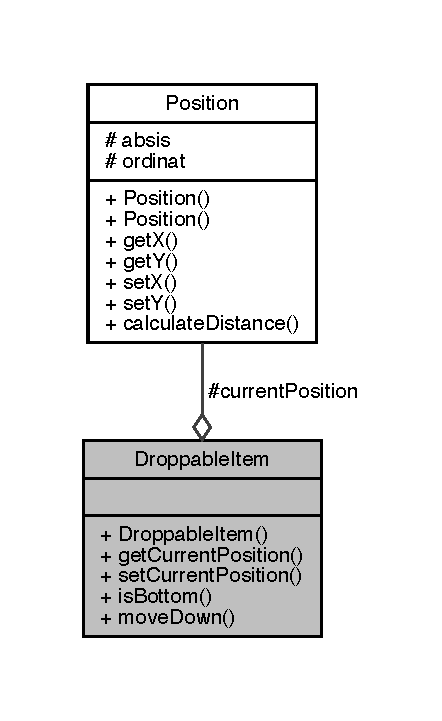
\includegraphics[width=212pt]{class_droppable_item__coll__graph}
\end{center}
\end{figure}
\subsection*{Public Member Functions}
\begin{DoxyCompactItemize}
\item 
\mbox{\hyperlink{class_droppable_item_a107fe5746196496e9a5983cc95d9ef57}{Droppable\+Item}} (\mbox{\hyperlink{class_position}{Position}} initial\+Position)
\item 
\mbox{\hyperlink{class_position}{Position}} \mbox{\hyperlink{class_droppable_item_a90d927cd4460d9cd5e0070b000606cd3}{get\+Current\+Position}} ()
\item 
void \mbox{\hyperlink{class_droppable_item_a8064bb69947880b73bf164ed8c73eaef}{set\+Current\+Position}} (\mbox{\hyperlink{class_position}{Position}} \mbox{\hyperlink{class_droppable_item_a9215c9fa588c9bd5aae4da387121b75c}{current\+Position}})
\item 
boolean \mbox{\hyperlink{class_droppable_item_a5cbe880513fffe6c70678bd3b86ca934}{is\+Bottom}} ()
\item 
void \mbox{\hyperlink{class_droppable_item_ac1870d36f1861a4574414355983d56c5}{move\+Down}} ()
\end{DoxyCompactItemize}
\subsection*{Protected Attributes}
\begin{DoxyCompactItemize}
\item 
\mbox{\hyperlink{class_position}{Position}} \mbox{\hyperlink{class_droppable_item_a9215c9fa588c9bd5aae4da387121b75c}{current\+Position}}
\end{DoxyCompactItemize}


\subsection{Detailed Description}
Represent object that will only move downwards. \begin{DoxyVersion}{Version}
1.\+0. 
\end{DoxyVersion}


\subsection{Constructor \& Destructor Documentation}
\mbox{\Hypertarget{class_droppable_item_a107fe5746196496e9a5983cc95d9ef57}\label{class_droppable_item_a107fe5746196496e9a5983cc95d9ef57}} 
\index{Droppable\+Item@{Droppable\+Item}!Droppable\+Item@{Droppable\+Item}}
\index{Droppable\+Item@{Droppable\+Item}!Droppable\+Item@{Droppable\+Item}}
\subsubsection{\texorpdfstring{Droppable\+Item()}{DroppableItem()}}
{\footnotesize\ttfamily Droppable\+Item.\+Droppable\+Item (\begin{DoxyParamCaption}\item[{\mbox{\hyperlink{class_position}{Position}}}]{initial\+Position }\end{DoxyParamCaption})\hspace{0.3cm}{\ttfamily [inline]}}

Constructor. 
\begin{DoxyParams}{Parameters}
{\em initial\+Position} & the initial position of the item. \\
\hline
\end{DoxyParams}


\subsection{Member Function Documentation}
\mbox{\Hypertarget{class_droppable_item_a90d927cd4460d9cd5e0070b000606cd3}\label{class_droppable_item_a90d927cd4460d9cd5e0070b000606cd3}} 
\index{Droppable\+Item@{Droppable\+Item}!get\+Current\+Position@{get\+Current\+Position}}
\index{get\+Current\+Position@{get\+Current\+Position}!Droppable\+Item@{Droppable\+Item}}
\subsubsection{\texorpdfstring{get\+Current\+Position()}{getCurrentPosition()}}
{\footnotesize\ttfamily \mbox{\hyperlink{class_position}{Position}} Droppable\+Item.\+get\+Current\+Position (\begin{DoxyParamCaption}{ }\end{DoxyParamCaption})\hspace{0.3cm}{\ttfamily [inline]}}

current\+Position getter. \begin{DoxyReturn}{Returns}
object of \mbox{\hyperlink{class_position}{Position}}. 
\end{DoxyReturn}
\mbox{\Hypertarget{class_droppable_item_a5cbe880513fffe6c70678bd3b86ca934}\label{class_droppable_item_a5cbe880513fffe6c70678bd3b86ca934}} 
\index{Droppable\+Item@{Droppable\+Item}!is\+Bottom@{is\+Bottom}}
\index{is\+Bottom@{is\+Bottom}!Droppable\+Item@{Droppable\+Item}}
\subsubsection{\texorpdfstring{is\+Bottom()}{isBottom()}}
{\footnotesize\ttfamily boolean Droppable\+Item.\+is\+Bottom (\begin{DoxyParamCaption}{ }\end{DoxyParamCaption})\hspace{0.3cm}{\ttfamily [inline]}}

check whether the droppable item is in bottom. \begin{DoxyReturn}{Returns}
boolean. 
\end{DoxyReturn}
Here is the call graph for this function\+:
\nopagebreak
\begin{figure}[H]
\begin{center}
\leavevmode
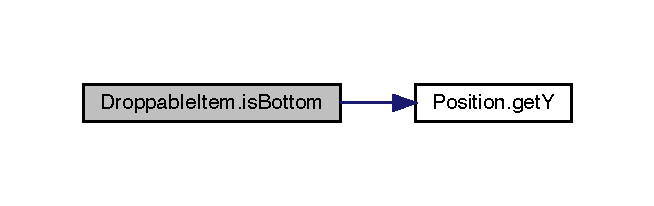
\includegraphics[width=314pt]{class_droppable_item_a5cbe880513fffe6c70678bd3b86ca934_cgraph}
\end{center}
\end{figure}
\mbox{\Hypertarget{class_droppable_item_ac1870d36f1861a4574414355983d56c5}\label{class_droppable_item_ac1870d36f1861a4574414355983d56c5}} 
\index{Droppable\+Item@{Droppable\+Item}!move\+Down@{move\+Down}}
\index{move\+Down@{move\+Down}!Droppable\+Item@{Droppable\+Item}}
\subsubsection{\texorpdfstring{move\+Down()}{moveDown()}}
{\footnotesize\ttfamily void Droppable\+Item.\+move\+Down (\begin{DoxyParamCaption}{ }\end{DoxyParamCaption})\hspace{0.3cm}{\ttfamily [inline]}}

move object downwards. Here is the call graph for this function\+:
\nopagebreak
\begin{figure}[H]
\begin{center}
\leavevmode
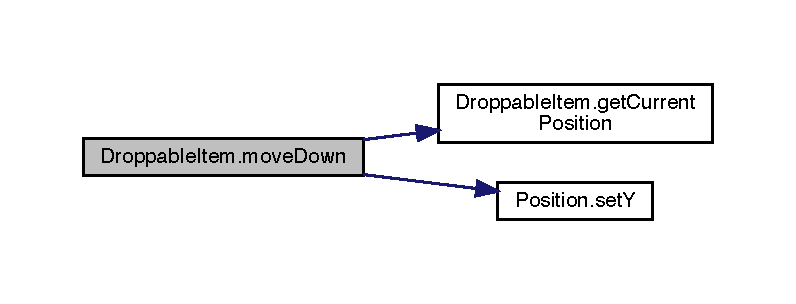
\includegraphics[width=350pt]{class_droppable_item_ac1870d36f1861a4574414355983d56c5_cgraph}
\end{center}
\end{figure}
\mbox{\Hypertarget{class_droppable_item_a8064bb69947880b73bf164ed8c73eaef}\label{class_droppable_item_a8064bb69947880b73bf164ed8c73eaef}} 
\index{Droppable\+Item@{Droppable\+Item}!set\+Current\+Position@{set\+Current\+Position}}
\index{set\+Current\+Position@{set\+Current\+Position}!Droppable\+Item@{Droppable\+Item}}
\subsubsection{\texorpdfstring{set\+Current\+Position()}{setCurrentPosition()}}
{\footnotesize\ttfamily void Droppable\+Item.\+set\+Current\+Position (\begin{DoxyParamCaption}\item[{\mbox{\hyperlink{class_position}{Position}}}]{current\+Position }\end{DoxyParamCaption})\hspace{0.3cm}{\ttfamily [inline]}}

current\+Position\+Setter. 
\begin{DoxyParams}{Parameters}
{\em current\+Position} & object of \mbox{\hyperlink{class_position}{Position}} to be set. \\
\hline
\end{DoxyParams}


\subsection{Member Data Documentation}
\mbox{\Hypertarget{class_droppable_item_a9215c9fa588c9bd5aae4da387121b75c}\label{class_droppable_item_a9215c9fa588c9bd5aae4da387121b75c}} 
\index{Droppable\+Item@{Droppable\+Item}!current\+Position@{current\+Position}}
\index{current\+Position@{current\+Position}!Droppable\+Item@{Droppable\+Item}}
\subsubsection{\texorpdfstring{current\+Position}{currentPosition}}
{\footnotesize\ttfamily \mbox{\hyperlink{class_position}{Position}} Droppable\+Item.\+current\+Position\hspace{0.3cm}{\ttfamily [protected]}}



The documentation for this class was generated from the following file\+:\begin{DoxyCompactItemize}
\item 
\mbox{\hyperlink{_droppable_item_8java}{Droppable\+Item.\+java}}\end{DoxyCompactItemize}

\hypertarget{class_droppable_item_test}{}\section{Droppable\+Item\+Test Class Reference}
\label{class_droppable_item_test}\index{Droppable\+Item\+Test@{Droppable\+Item\+Test}}


Collaboration diagram for Droppable\+Item\+Test\+:
\nopagebreak
\begin{figure}[H]
\begin{center}
\leavevmode
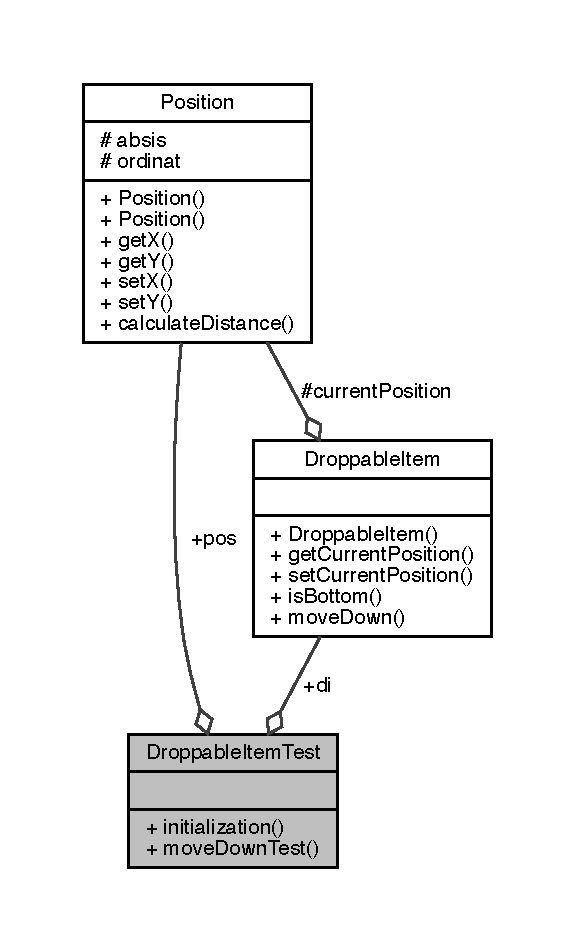
\includegraphics[width=276pt]{class_droppable_item_test__coll__graph}
\end{center}
\end{figure}
\subsection*{Public Member Functions}
\begin{DoxyCompactItemize}
\item 
void \mbox{\hyperlink{class_droppable_item_test_a21fe6227c90bc306be2cc17a857d6120}{initialization}} ()
\item 
void \mbox{\hyperlink{class_droppable_item_test_a6cf1fa022a5a09f02c6674dc66db4efb}{move\+Down\+Test}} ()
\end{DoxyCompactItemize}
\subsection*{Public Attributes}
\begin{DoxyCompactItemize}
\item 
\mbox{\hyperlink{class_position}{Position}} \mbox{\hyperlink{class_droppable_item_test_adad841a7c8ecced949d2b2d925163e5a}{pos}}
\item 
\mbox{\hyperlink{class_droppable_item}{Droppable\+Item}} \mbox{\hyperlink{class_droppable_item_test_a27f44f35ae846f3fec4c0c526d465340}{di}}
\end{DoxyCompactItemize}


\subsection{Member Function Documentation}
\mbox{\Hypertarget{class_droppable_item_test_a21fe6227c90bc306be2cc17a857d6120}\label{class_droppable_item_test_a21fe6227c90bc306be2cc17a857d6120}} 
\index{Droppable\+Item\+Test@{Droppable\+Item\+Test}!initialization@{initialization}}
\index{initialization@{initialization}!Droppable\+Item\+Test@{Droppable\+Item\+Test}}
\subsubsection{\texorpdfstring{initialization()}{initialization()}}
{\footnotesize\ttfamily void Droppable\+Item\+Test.\+initialization (\begin{DoxyParamCaption}{ }\end{DoxyParamCaption})\hspace{0.3cm}{\ttfamily [inline]}}

\mbox{\Hypertarget{class_droppable_item_test_a6cf1fa022a5a09f02c6674dc66db4efb}\label{class_droppable_item_test_a6cf1fa022a5a09f02c6674dc66db4efb}} 
\index{Droppable\+Item\+Test@{Droppable\+Item\+Test}!move\+Down\+Test@{move\+Down\+Test}}
\index{move\+Down\+Test@{move\+Down\+Test}!Droppable\+Item\+Test@{Droppable\+Item\+Test}}
\subsubsection{\texorpdfstring{move\+Down\+Test()}{moveDownTest()}}
{\footnotesize\ttfamily void Droppable\+Item\+Test.\+move\+Down\+Test (\begin{DoxyParamCaption}{ }\end{DoxyParamCaption})\hspace{0.3cm}{\ttfamily [inline]}}

Here is the call graph for this function\+:
\nopagebreak
\begin{figure}[H]
\begin{center}
\leavevmode
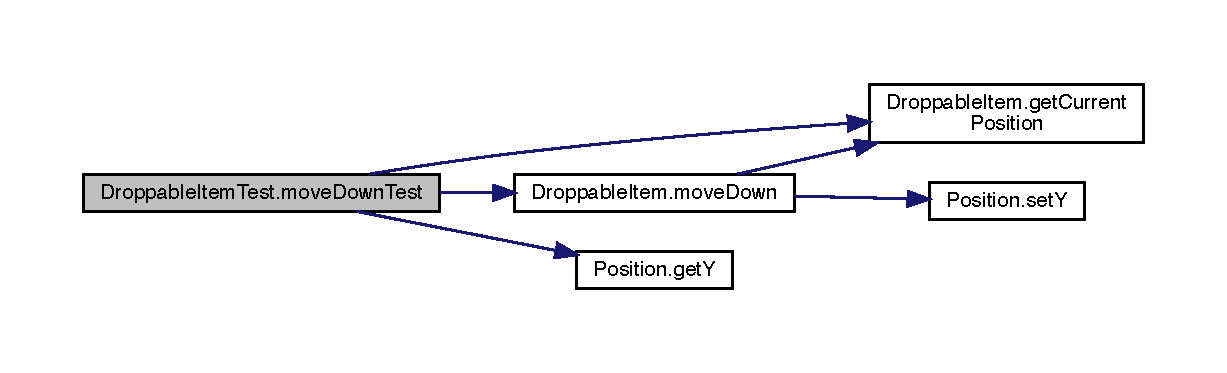
\includegraphics[width=350pt]{class_droppable_item_test_a6cf1fa022a5a09f02c6674dc66db4efb_cgraph}
\end{center}
\end{figure}


\subsection{Member Data Documentation}
\mbox{\Hypertarget{class_droppable_item_test_a27f44f35ae846f3fec4c0c526d465340}\label{class_droppable_item_test_a27f44f35ae846f3fec4c0c526d465340}} 
\index{Droppable\+Item\+Test@{Droppable\+Item\+Test}!di@{di}}
\index{di@{di}!Droppable\+Item\+Test@{Droppable\+Item\+Test}}
\subsubsection{\texorpdfstring{di}{di}}
{\footnotesize\ttfamily \mbox{\hyperlink{class_droppable_item}{Droppable\+Item}} Droppable\+Item\+Test.\+di}

\mbox{\Hypertarget{class_droppable_item_test_adad841a7c8ecced949d2b2d925163e5a}\label{class_droppable_item_test_adad841a7c8ecced949d2b2d925163e5a}} 
\index{Droppable\+Item\+Test@{Droppable\+Item\+Test}!pos@{pos}}
\index{pos@{pos}!Droppable\+Item\+Test@{Droppable\+Item\+Test}}
\subsubsection{\texorpdfstring{pos}{pos}}
{\footnotesize\ttfamily \mbox{\hyperlink{class_position}{Position}} Droppable\+Item\+Test.\+pos}



The documentation for this class was generated from the following file\+:\begin{DoxyCompactItemize}
\item 
\mbox{\hyperlink{_droppable_item_test_8java}{Droppable\+Item\+Test.\+java}}\end{DoxyCompactItemize}

\hypertarget{class_fish}{}\section{Fish Class Reference}
\label{class_fish}\index{Fish@{Fish}}


Inheritance diagram for Fish\+:
\nopagebreak
\begin{figure}[H]
\begin{center}
\leavevmode
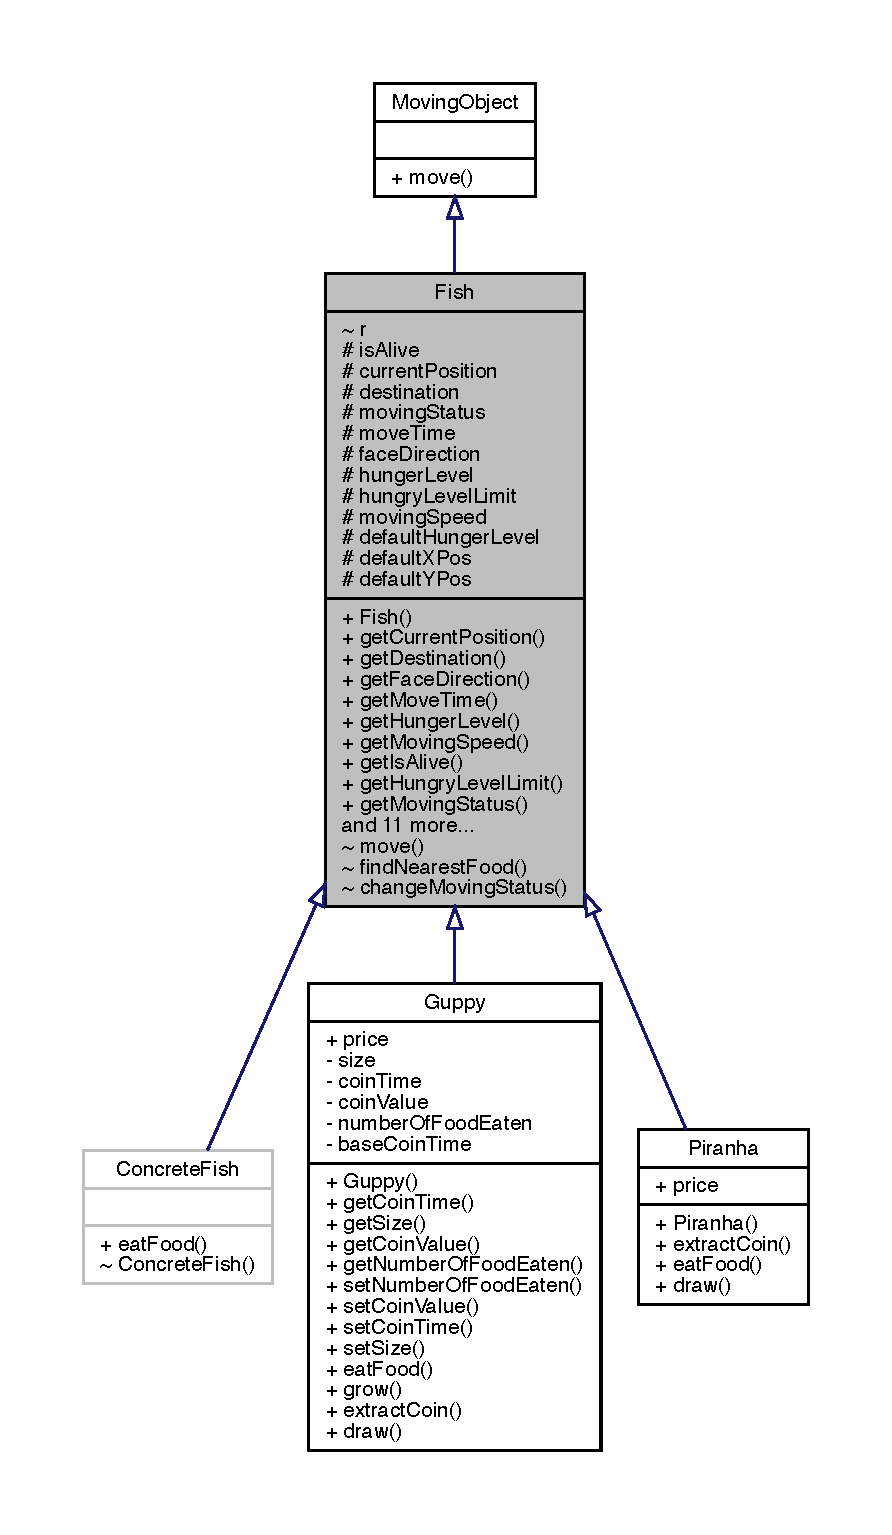
\includegraphics[height=550pt]{class_fish__inherit__graph}
\end{center}
\end{figure}


Collaboration diagram for Fish\+:
\nopagebreak
\begin{figure}[H]
\begin{center}
\leavevmode
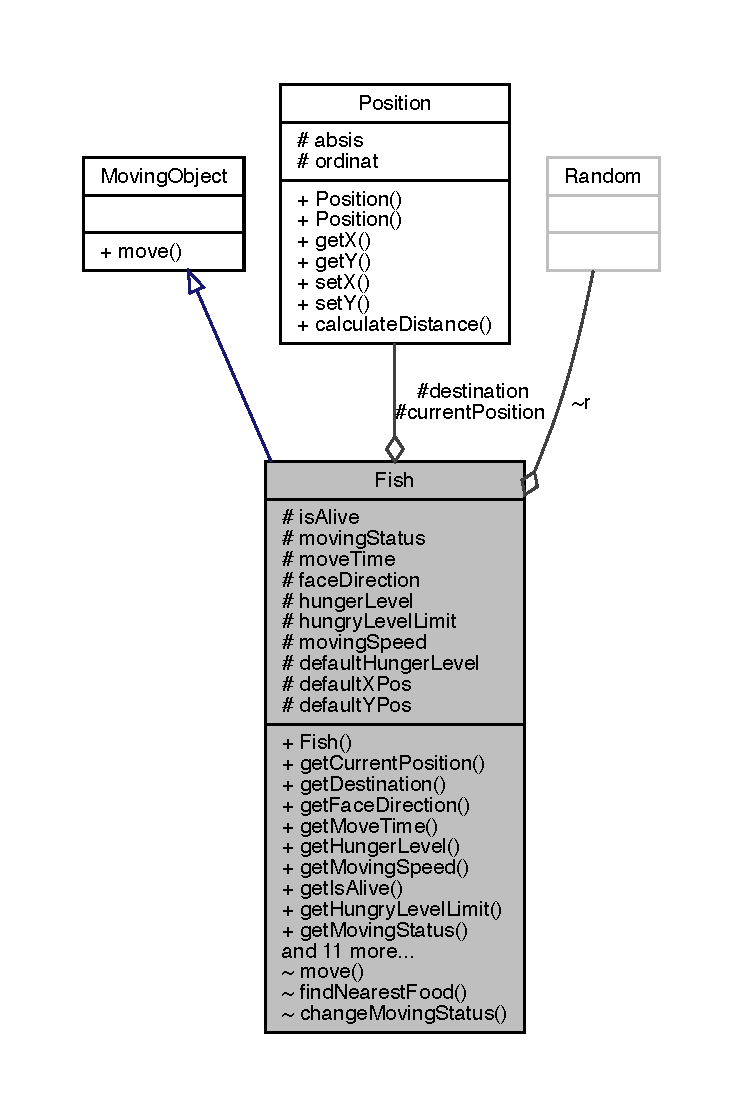
\includegraphics[width=350pt]{class_fish__coll__graph}
\end{center}
\end{figure}
\subsection*{Public Member Functions}
\begin{DoxyCompactItemize}
\item 
\mbox{\hyperlink{class_fish_ae9ad0ceab4b720f2c37a4fd4693bdd2f}{Fish}} ()
\item 
\mbox{\hyperlink{class_position}{Position}} \mbox{\hyperlink{class_fish_afc0c0824c91f3bbb61fc3762b08d9137}{get\+Current\+Position}} ()
\item 
\mbox{\hyperlink{class_position}{Position}} \mbox{\hyperlink{class_fish_a39feef3e603de6ea5931ada8b3e1e27d}{get\+Destination}} ()
\item 
boolean \mbox{\hyperlink{class_fish_a5ed789451c5b7fc9808de4837f06eb02}{get\+Face\+Direction}} ()
\item 
double \mbox{\hyperlink{class_fish_a9e32f70d5f02b4d0fb7e5f0e92e9bf4e}{get\+Move\+Time}} ()
\item 
int \mbox{\hyperlink{class_fish_a6b0fb4a552039ab06338470584bd838b}{get\+Hunger\+Level}} ()
\item 
int \mbox{\hyperlink{class_fish_a256fe3bcc998d4d668e8917e8a453e7a}{get\+Moving\+Speed}} ()
\item 
boolean \mbox{\hyperlink{class_fish_a8c7a1a1666af0c425a9ef0e83d33779c}{get\+Is\+Alive}} ()
\item 
int \mbox{\hyperlink{class_fish_aa121fc4335ac49aa48e4ef9e137c0e8b}{get\+Hungry\+Level\+Limit}} ()
\item 
\mbox{\hyperlink{enum_moving_object_1_1_moving_status}{Moving\+Status}} \mbox{\hyperlink{class_fish_a5abbd7e198b7770b666a85c5b02f6501}{get\+Moving\+Status}} ()
\item 
void \mbox{\hyperlink{class_fish_ab86ec00d2b503f310f1c29bc9a94fbd7}{set\+Current\+Position}} (\mbox{\hyperlink{class_position}{Position}} \mbox{\hyperlink{class_fish_a1f025627baa1802f78dab5fef88b7838}{current\+Position}})
\item 
void \mbox{\hyperlink{class_fish_a9b74ce69e55149c7df9f70e83ce5b66b}{set\+Destination}} (\mbox{\hyperlink{class_position}{Position}} \mbox{\hyperlink{class_fish_a93523126df751dd0301a1fcf2ed42735}{destination}})
\item 
void \mbox{\hyperlink{class_fish_a95e9975f718a7a24254bcbb58dfe1ba1}{set\+Hunger\+Level}} (int \mbox{\hyperlink{class_fish_a9e0224f04ab5b9da07414075698bbbf1}{hunger\+Level}})
\item 
void \mbox{\hyperlink{class_fish_ad6d23a97f4d4f6916243cf0033470e87}{set\+Move\+Time}} (int \mbox{\hyperlink{class_fish_a630f9859f38f851ccdf223daebebd27f}{move\+Time}})
\item 
void \mbox{\hyperlink{class_fish_afcc56cacfeded2fb41f3de811aff9d45}{set\+Moving\+Status}} (\mbox{\hyperlink{enum_moving_object_1_1_moving_status}{Moving\+Status}} \mbox{\hyperlink{class_fish_adb3e06c4c9cfd4e55a7d819c50702521}{moving\+Status}})
\item 
void \mbox{\hyperlink{class_fish_a88fa149bd62388b1aee597c9ec540369}{change\+Is\+Alive}} ()
\item 
void \mbox{\hyperlink{class_fish_a9fb18733f43c29b1a4c4b16a6322aec6}{change\+Face\+Direction}} ()
\item 
boolean \mbox{\hyperlink{class_fish_aa4d669d1ffe1655a62c8b9ea5c477d72}{is\+Hungry}} ()
\item 
void \mbox{\hyperlink{class_fish_a8ac2c9963873520d435ee1609dae0174}{move\+Hunt}} (\mbox{\hyperlink{class_position}{Position}} \mbox{\hyperlink{class_fish_a93523126df751dd0301a1fcf2ed42735}{destination}})
\item 
void \mbox{\hyperlink{class_fish_aa3683716f71b574717c30f0f7be3ec33}{move\+Random}} (\mbox{\hyperlink{class_position}{Position}} \mbox{\hyperlink{class_fish_a93523126df751dd0301a1fcf2ed42735}{destination}})
\item 
abstract void \mbox{\hyperlink{class_fish_af226ad690f56674f1b08d9d9562dde83}{eat\+Food}} ()
\end{DoxyCompactItemize}
\subsection*{Protected Attributes}
\begin{DoxyCompactItemize}
\item 
boolean \mbox{\hyperlink{class_fish_ad380340280b30f5700d206739b793d8f}{is\+Alive}}
\item 
\mbox{\hyperlink{class_position}{Position}} \mbox{\hyperlink{class_fish_a1f025627baa1802f78dab5fef88b7838}{current\+Position}}
\item 
\mbox{\hyperlink{class_position}{Position}} \mbox{\hyperlink{class_fish_a93523126df751dd0301a1fcf2ed42735}{destination}}
\item 
\mbox{\hyperlink{enum_moving_object_1_1_moving_status}{Moving\+Status}} \mbox{\hyperlink{class_fish_adb3e06c4c9cfd4e55a7d819c50702521}{moving\+Status}}
\item 
double \mbox{\hyperlink{class_fish_a630f9859f38f851ccdf223daebebd27f}{move\+Time}}
\item 
boolean \mbox{\hyperlink{class_fish_af86c6cd526847bf6be39c9cc170e5305}{face\+Direction}}
\item 
int \mbox{\hyperlink{class_fish_a9e0224f04ab5b9da07414075698bbbf1}{hunger\+Level}}
\item 
final int \mbox{\hyperlink{class_fish_a9d334546607726c92bc7e9a6ffd03f75}{hungry\+Level\+Limit}} = 40
\item 
final int \mbox{\hyperlink{class_fish_a9f5b20fab06597fda40be4c4d42473d0}{moving\+Speed}} = 1
\item 
final int \mbox{\hyperlink{class_fish_abb83de49d7a7fc239d603e11215e90f9}{default\+Hunger\+Level}} = 60
\item 
final double \mbox{\hyperlink{class_fish_a8b71b4abb80a350eca229e1f4c6656c4}{default\+X\+Pos}} = 0.\+0
\item 
final double \mbox{\hyperlink{class_fish_a9ce14817daae461df29a23d247c87a80}{default\+Y\+Pos}} = 0.\+0
\end{DoxyCompactItemize}


\subsection{Detailed Description}
Represent a fish. \begin{DoxyVersion}{Version}
1.\+0. 
\end{DoxyVersion}


\subsection{Constructor \& Destructor Documentation}
\mbox{\Hypertarget{class_fish_ae9ad0ceab4b720f2c37a4fd4693bdd2f}\label{class_fish_ae9ad0ceab4b720f2c37a4fd4693bdd2f}} 
\index{Fish@{Fish}!Fish@{Fish}}
\index{Fish@{Fish}!Fish@{Fish}}
\subsubsection{\texorpdfstring{Fish()}{Fish()}}
{\footnotesize\ttfamily Fish.\+Fish (\begin{DoxyParamCaption}{ }\end{DoxyParamCaption})\hspace{0.3cm}{\ttfamily [inline]}}

Constructor. 

\subsection{Member Function Documentation}
\mbox{\Hypertarget{class_fish_a9fb18733f43c29b1a4c4b16a6322aec6}\label{class_fish_a9fb18733f43c29b1a4c4b16a6322aec6}} 
\index{Fish@{Fish}!change\+Face\+Direction@{change\+Face\+Direction}}
\index{change\+Face\+Direction@{change\+Face\+Direction}!Fish@{Fish}}
\subsubsection{\texorpdfstring{change\+Face\+Direction()}{changeFaceDirection()}}
{\footnotesize\ttfamily void Fish.\+change\+Face\+Direction (\begin{DoxyParamCaption}{ }\end{DoxyParamCaption})\hspace{0.3cm}{\ttfamily [inline]}}

face\+Direction setter. Reverse the face\+Direction. \mbox{\Hypertarget{class_fish_a88fa149bd62388b1aee597c9ec540369}\label{class_fish_a88fa149bd62388b1aee597c9ec540369}} 
\index{Fish@{Fish}!change\+Is\+Alive@{change\+Is\+Alive}}
\index{change\+Is\+Alive@{change\+Is\+Alive}!Fish@{Fish}}
\subsubsection{\texorpdfstring{change\+Is\+Alive()}{changeIsAlive()}}
{\footnotesize\ttfamily void Fish.\+change\+Is\+Alive (\begin{DoxyParamCaption}{ }\end{DoxyParamCaption})\hspace{0.3cm}{\ttfamily [inline]}}

Change is\+Alive if fish hunger level below 0. Here is the call graph for this function\+:
\nopagebreak
\begin{figure}[H]
\begin{center}
\leavevmode
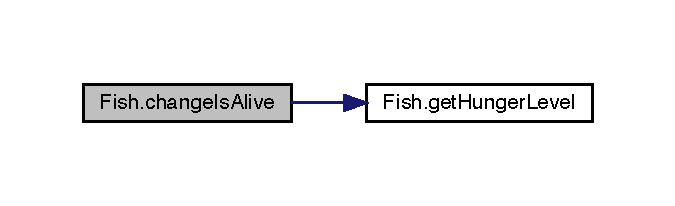
\includegraphics[width=324pt]{class_fish_a88fa149bd62388b1aee597c9ec540369_cgraph}
\end{center}
\end{figure}
\mbox{\Hypertarget{class_fish_af226ad690f56674f1b08d9d9562dde83}\label{class_fish_af226ad690f56674f1b08d9d9562dde83}} 
\index{Fish@{Fish}!eat\+Food@{eat\+Food}}
\index{eat\+Food@{eat\+Food}!Fish@{Fish}}
\subsubsection{\texorpdfstring{eat\+Food()}{eatFood()}}
{\footnotesize\ttfamily abstract void Fish.\+eat\+Food (\begin{DoxyParamCaption}{ }\end{DoxyParamCaption})\hspace{0.3cm}{\ttfamily [abstract]}}

eat food. \mbox{\Hypertarget{class_fish_afc0c0824c91f3bbb61fc3762b08d9137}\label{class_fish_afc0c0824c91f3bbb61fc3762b08d9137}} 
\index{Fish@{Fish}!get\+Current\+Position@{get\+Current\+Position}}
\index{get\+Current\+Position@{get\+Current\+Position}!Fish@{Fish}}
\subsubsection{\texorpdfstring{get\+Current\+Position()}{getCurrentPosition()}}
{\footnotesize\ttfamily \mbox{\hyperlink{class_position}{Position}} Fish.\+get\+Current\+Position (\begin{DoxyParamCaption}{ }\end{DoxyParamCaption})\hspace{0.3cm}{\ttfamily [inline]}}

current\+Position getter. \begin{DoxyReturn}{Returns}
object of \mbox{\hyperlink{class_position}{Position}}. 
\end{DoxyReturn}
\mbox{\Hypertarget{class_fish_a39feef3e603de6ea5931ada8b3e1e27d}\label{class_fish_a39feef3e603de6ea5931ada8b3e1e27d}} 
\index{Fish@{Fish}!get\+Destination@{get\+Destination}}
\index{get\+Destination@{get\+Destination}!Fish@{Fish}}
\subsubsection{\texorpdfstring{get\+Destination()}{getDestination()}}
{\footnotesize\ttfamily \mbox{\hyperlink{class_position}{Position}} Fish.\+get\+Destination (\begin{DoxyParamCaption}{ }\end{DoxyParamCaption})\hspace{0.3cm}{\ttfamily [inline]}}

destination getter. \begin{DoxyReturn}{Returns}
object of \mbox{\hyperlink{class_position}{Position}}. 
\end{DoxyReturn}
\mbox{\Hypertarget{class_fish_a5ed789451c5b7fc9808de4837f06eb02}\label{class_fish_a5ed789451c5b7fc9808de4837f06eb02}} 
\index{Fish@{Fish}!get\+Face\+Direction@{get\+Face\+Direction}}
\index{get\+Face\+Direction@{get\+Face\+Direction}!Fish@{Fish}}
\subsubsection{\texorpdfstring{get\+Face\+Direction()}{getFaceDirection()}}
{\footnotesize\ttfamily boolean Fish.\+get\+Face\+Direction (\begin{DoxyParamCaption}{ }\end{DoxyParamCaption})\hspace{0.3cm}{\ttfamily [inline]}}

fish face direction getter, if true then left. \begin{DoxyReturn}{Returns}
boolean. 
\end{DoxyReturn}
\mbox{\Hypertarget{class_fish_a6b0fb4a552039ab06338470584bd838b}\label{class_fish_a6b0fb4a552039ab06338470584bd838b}} 
\index{Fish@{Fish}!get\+Hunger\+Level@{get\+Hunger\+Level}}
\index{get\+Hunger\+Level@{get\+Hunger\+Level}!Fish@{Fish}}
\subsubsection{\texorpdfstring{get\+Hunger\+Level()}{getHungerLevel()}}
{\footnotesize\ttfamily int Fish.\+get\+Hunger\+Level (\begin{DoxyParamCaption}{ }\end{DoxyParamCaption})\hspace{0.3cm}{\ttfamily [inline]}}

hunger\+Level getter. \begin{DoxyReturn}{Returns}
integer. 
\end{DoxyReturn}
\mbox{\Hypertarget{class_fish_aa121fc4335ac49aa48e4ef9e137c0e8b}\label{class_fish_aa121fc4335ac49aa48e4ef9e137c0e8b}} 
\index{Fish@{Fish}!get\+Hungry\+Level\+Limit@{get\+Hungry\+Level\+Limit}}
\index{get\+Hungry\+Level\+Limit@{get\+Hungry\+Level\+Limit}!Fish@{Fish}}
\subsubsection{\texorpdfstring{get\+Hungry\+Level\+Limit()}{getHungryLevelLimit()}}
{\footnotesize\ttfamily int Fish.\+get\+Hungry\+Level\+Limit (\begin{DoxyParamCaption}{ }\end{DoxyParamCaption})\hspace{0.3cm}{\ttfamily [inline]}}

hungry\+Level\+Limit getter. \begin{DoxyReturn}{Returns}
integer. 
\end{DoxyReturn}
\mbox{\Hypertarget{class_fish_a8c7a1a1666af0c425a9ef0e83d33779c}\label{class_fish_a8c7a1a1666af0c425a9ef0e83d33779c}} 
\index{Fish@{Fish}!get\+Is\+Alive@{get\+Is\+Alive}}
\index{get\+Is\+Alive@{get\+Is\+Alive}!Fish@{Fish}}
\subsubsection{\texorpdfstring{get\+Is\+Alive()}{getIsAlive()}}
{\footnotesize\ttfamily boolean Fish.\+get\+Is\+Alive (\begin{DoxyParamCaption}{ }\end{DoxyParamCaption})\hspace{0.3cm}{\ttfamily [inline]}}

is\+Alive getter. \begin{DoxyReturn}{Returns}
boolean, if true then still alive. 
\end{DoxyReturn}
\mbox{\Hypertarget{class_fish_a9e32f70d5f02b4d0fb7e5f0e92e9bf4e}\label{class_fish_a9e32f70d5f02b4d0fb7e5f0e92e9bf4e}} 
\index{Fish@{Fish}!get\+Move\+Time@{get\+Move\+Time}}
\index{get\+Move\+Time@{get\+Move\+Time}!Fish@{Fish}}
\subsubsection{\texorpdfstring{get\+Move\+Time()}{getMoveTime()}}
{\footnotesize\ttfamily double Fish.\+get\+Move\+Time (\begin{DoxyParamCaption}{ }\end{DoxyParamCaption})\hspace{0.3cm}{\ttfamily [inline]}}

move\+Time getter. \begin{DoxyReturn}{Returns}
double. 
\end{DoxyReturn}
\mbox{\Hypertarget{class_fish_a256fe3bcc998d4d668e8917e8a453e7a}\label{class_fish_a256fe3bcc998d4d668e8917e8a453e7a}} 
\index{Fish@{Fish}!get\+Moving\+Speed@{get\+Moving\+Speed}}
\index{get\+Moving\+Speed@{get\+Moving\+Speed}!Fish@{Fish}}
\subsubsection{\texorpdfstring{get\+Moving\+Speed()}{getMovingSpeed()}}
{\footnotesize\ttfamily int Fish.\+get\+Moving\+Speed (\begin{DoxyParamCaption}{ }\end{DoxyParamCaption})\hspace{0.3cm}{\ttfamily [inline]}}

moving\+Speed getter. \begin{DoxyReturn}{Returns}
integer. 
\end{DoxyReturn}
\mbox{\Hypertarget{class_fish_a5abbd7e198b7770b666a85c5b02f6501}\label{class_fish_a5abbd7e198b7770b666a85c5b02f6501}} 
\index{Fish@{Fish}!get\+Moving\+Status@{get\+Moving\+Status}}
\index{get\+Moving\+Status@{get\+Moving\+Status}!Fish@{Fish}}
\subsubsection{\texorpdfstring{get\+Moving\+Status()}{getMovingStatus()}}
{\footnotesize\ttfamily \mbox{\hyperlink{enum_moving_object_1_1_moving_status}{Moving\+Status}} Fish.\+get\+Moving\+Status (\begin{DoxyParamCaption}{ }\end{DoxyParamCaption})\hspace{0.3cm}{\ttfamily [inline]}}

moving\+Status getter. \begin{DoxyReturn}{Returns}
Moving\+Status enum. 
\end{DoxyReturn}
\mbox{\Hypertarget{class_fish_aa4d669d1ffe1655a62c8b9ea5c477d72}\label{class_fish_aa4d669d1ffe1655a62c8b9ea5c477d72}} 
\index{Fish@{Fish}!is\+Hungry@{is\+Hungry}}
\index{is\+Hungry@{is\+Hungry}!Fish@{Fish}}
\subsubsection{\texorpdfstring{is\+Hungry()}{isHungry()}}
{\footnotesize\ttfamily boolean Fish.\+is\+Hungry (\begin{DoxyParamCaption}{ }\end{DoxyParamCaption})\hspace{0.3cm}{\ttfamily [inline]}}

\mbox{\hyperlink{class_fish}{Fish}} hungry checker. \begin{DoxyReturn}{Returns}
true if fish hungry. 
\end{DoxyReturn}
\mbox{\Hypertarget{class_fish_a8ac2c9963873520d435ee1609dae0174}\label{class_fish_a8ac2c9963873520d435ee1609dae0174}} 
\index{Fish@{Fish}!move\+Hunt@{move\+Hunt}}
\index{move\+Hunt@{move\+Hunt}!Fish@{Fish}}
\subsubsection{\texorpdfstring{move\+Hunt()}{moveHunt()}}
{\footnotesize\ttfamily void Fish.\+move\+Hunt (\begin{DoxyParamCaption}\item[{\mbox{\hyperlink{class_position}{Position}}}]{destination }\end{DoxyParamCaption})\hspace{0.3cm}{\ttfamily [inline]}}

move fish towards nearest food. 
\begin{DoxyParams}{Parameters}
{\em destination} & nearest food position. \\
\hline
\end{DoxyParams}
Here is the call graph for this function\+:
\nopagebreak
\begin{figure}[H]
\begin{center}
\leavevmode
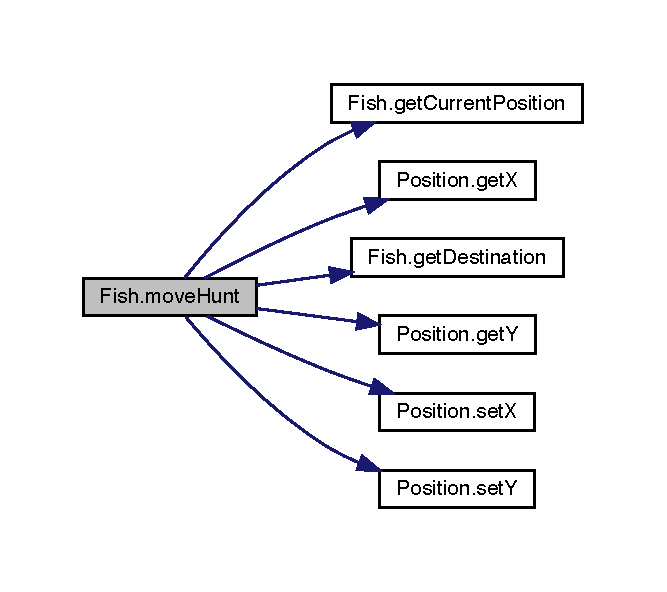
\includegraphics[width=320pt]{class_fish_a8ac2c9963873520d435ee1609dae0174_cgraph}
\end{center}
\end{figure}
\mbox{\Hypertarget{class_fish_aa3683716f71b574717c30f0f7be3ec33}\label{class_fish_aa3683716f71b574717c30f0f7be3ec33}} 
\index{Fish@{Fish}!move\+Random@{move\+Random}}
\index{move\+Random@{move\+Random}!Fish@{Fish}}
\subsubsection{\texorpdfstring{move\+Random()}{moveRandom()}}
{\footnotesize\ttfamily void Fish.\+move\+Random (\begin{DoxyParamCaption}\item[{\mbox{\hyperlink{class_position}{Position}}}]{destination }\end{DoxyParamCaption})\hspace{0.3cm}{\ttfamily [inline]}}

move to random position. 
\begin{DoxyParams}{Parameters}
{\em destination} & random position. \\
\hline
\end{DoxyParams}
Here is the call graph for this function\+:
\nopagebreak
\begin{figure}[H]
\begin{center}
\leavevmode
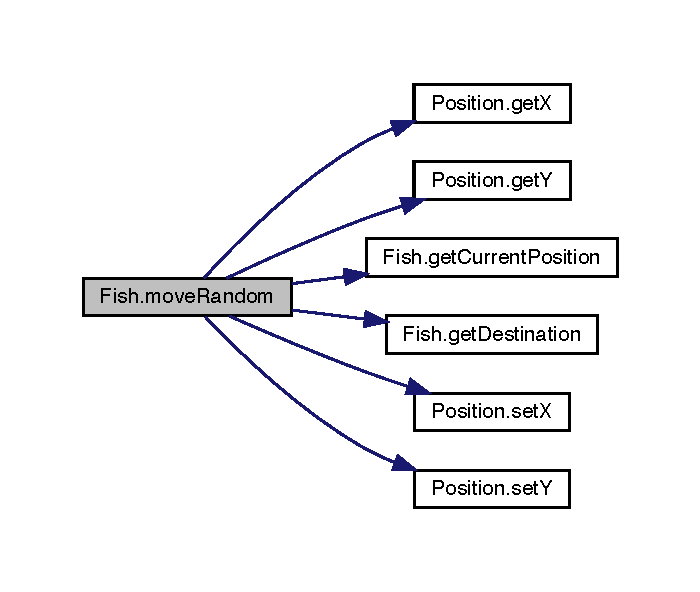
\includegraphics[width=336pt]{class_fish_aa3683716f71b574717c30f0f7be3ec33_cgraph}
\end{center}
\end{figure}
\mbox{\Hypertarget{class_fish_ab86ec00d2b503f310f1c29bc9a94fbd7}\label{class_fish_ab86ec00d2b503f310f1c29bc9a94fbd7}} 
\index{Fish@{Fish}!set\+Current\+Position@{set\+Current\+Position}}
\index{set\+Current\+Position@{set\+Current\+Position}!Fish@{Fish}}
\subsubsection{\texorpdfstring{set\+Current\+Position()}{setCurrentPosition()}}
{\footnotesize\ttfamily void Fish.\+set\+Current\+Position (\begin{DoxyParamCaption}\item[{\mbox{\hyperlink{class_position}{Position}}}]{current\+Position }\end{DoxyParamCaption})\hspace{0.3cm}{\ttfamily [inline]}}

current\+Position setter. 
\begin{DoxyParams}{Parameters}
{\em current\+Position} & Object of \mbox{\hyperlink{class_position}{Position}}. \\
\hline
\end{DoxyParams}
\mbox{\Hypertarget{class_fish_a9b74ce69e55149c7df9f70e83ce5b66b}\label{class_fish_a9b74ce69e55149c7df9f70e83ce5b66b}} 
\index{Fish@{Fish}!set\+Destination@{set\+Destination}}
\index{set\+Destination@{set\+Destination}!Fish@{Fish}}
\subsubsection{\texorpdfstring{set\+Destination()}{setDestination()}}
{\footnotesize\ttfamily void Fish.\+set\+Destination (\begin{DoxyParamCaption}\item[{\mbox{\hyperlink{class_position}{Position}}}]{destination }\end{DoxyParamCaption})\hspace{0.3cm}{\ttfamily [inline]}}

destination setter. 
\begin{DoxyParams}{Parameters}
{\em destination} & Object of \mbox{\hyperlink{class_position}{Position}}. \\
\hline
\end{DoxyParams}
\mbox{\Hypertarget{class_fish_a95e9975f718a7a24254bcbb58dfe1ba1}\label{class_fish_a95e9975f718a7a24254bcbb58dfe1ba1}} 
\index{Fish@{Fish}!set\+Hunger\+Level@{set\+Hunger\+Level}}
\index{set\+Hunger\+Level@{set\+Hunger\+Level}!Fish@{Fish}}
\subsubsection{\texorpdfstring{set\+Hunger\+Level()}{setHungerLevel()}}
{\footnotesize\ttfamily void Fish.\+set\+Hunger\+Level (\begin{DoxyParamCaption}\item[{int}]{hunger\+Level }\end{DoxyParamCaption})\hspace{0.3cm}{\ttfamily [inline]}}

hunger\+Level setter. 
\begin{DoxyParams}{Parameters}
{\em hunger\+Level} & integer. \\
\hline
\end{DoxyParams}
\mbox{\Hypertarget{class_fish_ad6d23a97f4d4f6916243cf0033470e87}\label{class_fish_ad6d23a97f4d4f6916243cf0033470e87}} 
\index{Fish@{Fish}!set\+Move\+Time@{set\+Move\+Time}}
\index{set\+Move\+Time@{set\+Move\+Time}!Fish@{Fish}}
\subsubsection{\texorpdfstring{set\+Move\+Time()}{setMoveTime()}}
{\footnotesize\ttfamily void Fish.\+set\+Move\+Time (\begin{DoxyParamCaption}\item[{int}]{move\+Time }\end{DoxyParamCaption})\hspace{0.3cm}{\ttfamily [inline]}}

move\+Time setter. 
\begin{DoxyParams}{Parameters}
{\em move\+Time} & integer. \\
\hline
\end{DoxyParams}
\mbox{\Hypertarget{class_fish_afcc56cacfeded2fb41f3de811aff9d45}\label{class_fish_afcc56cacfeded2fb41f3de811aff9d45}} 
\index{Fish@{Fish}!set\+Moving\+Status@{set\+Moving\+Status}}
\index{set\+Moving\+Status@{set\+Moving\+Status}!Fish@{Fish}}
\subsubsection{\texorpdfstring{set\+Moving\+Status()}{setMovingStatus()}}
{\footnotesize\ttfamily void Fish.\+set\+Moving\+Status (\begin{DoxyParamCaption}\item[{\mbox{\hyperlink{enum_moving_object_1_1_moving_status}{Moving\+Status}}}]{moving\+Status }\end{DoxyParamCaption})\hspace{0.3cm}{\ttfamily [inline]}}

moving\+Status setter. 
\begin{DoxyParams}{Parameters}
{\em moving\+Status} & Moving\+Status enum. \\
\hline
\end{DoxyParams}


\subsection{Member Data Documentation}
\mbox{\Hypertarget{class_fish_a1f025627baa1802f78dab5fef88b7838}\label{class_fish_a1f025627baa1802f78dab5fef88b7838}} 
\index{Fish@{Fish}!current\+Position@{current\+Position}}
\index{current\+Position@{current\+Position}!Fish@{Fish}}
\subsubsection{\texorpdfstring{current\+Position}{currentPosition}}
{\footnotesize\ttfamily \mbox{\hyperlink{class_position}{Position}} Fish.\+current\+Position\hspace{0.3cm}{\ttfamily [protected]}}

\mbox{\Hypertarget{class_fish_abb83de49d7a7fc239d603e11215e90f9}\label{class_fish_abb83de49d7a7fc239d603e11215e90f9}} 
\index{Fish@{Fish}!default\+Hunger\+Level@{default\+Hunger\+Level}}
\index{default\+Hunger\+Level@{default\+Hunger\+Level}!Fish@{Fish}}
\subsubsection{\texorpdfstring{default\+Hunger\+Level}{defaultHungerLevel}}
{\footnotesize\ttfamily final int Fish.\+default\+Hunger\+Level = 60\hspace{0.3cm}{\ttfamily [protected]}}

\mbox{\Hypertarget{class_fish_a8b71b4abb80a350eca229e1f4c6656c4}\label{class_fish_a8b71b4abb80a350eca229e1f4c6656c4}} 
\index{Fish@{Fish}!default\+X\+Pos@{default\+X\+Pos}}
\index{default\+X\+Pos@{default\+X\+Pos}!Fish@{Fish}}
\subsubsection{\texorpdfstring{default\+X\+Pos}{defaultXPos}}
{\footnotesize\ttfamily final double Fish.\+default\+X\+Pos = 0.\+0\hspace{0.3cm}{\ttfamily [protected]}}

\mbox{\Hypertarget{class_fish_a9ce14817daae461df29a23d247c87a80}\label{class_fish_a9ce14817daae461df29a23d247c87a80}} 
\index{Fish@{Fish}!default\+Y\+Pos@{default\+Y\+Pos}}
\index{default\+Y\+Pos@{default\+Y\+Pos}!Fish@{Fish}}
\subsubsection{\texorpdfstring{default\+Y\+Pos}{defaultYPos}}
{\footnotesize\ttfamily final double Fish.\+default\+Y\+Pos = 0.\+0\hspace{0.3cm}{\ttfamily [protected]}}

\mbox{\Hypertarget{class_fish_a93523126df751dd0301a1fcf2ed42735}\label{class_fish_a93523126df751dd0301a1fcf2ed42735}} 
\index{Fish@{Fish}!destination@{destination}}
\index{destination@{destination}!Fish@{Fish}}
\subsubsection{\texorpdfstring{destination}{destination}}
{\footnotesize\ttfamily \mbox{\hyperlink{class_position}{Position}} Fish.\+destination\hspace{0.3cm}{\ttfamily [protected]}}

\mbox{\Hypertarget{class_fish_af86c6cd526847bf6be39c9cc170e5305}\label{class_fish_af86c6cd526847bf6be39c9cc170e5305}} 
\index{Fish@{Fish}!face\+Direction@{face\+Direction}}
\index{face\+Direction@{face\+Direction}!Fish@{Fish}}
\subsubsection{\texorpdfstring{face\+Direction}{faceDirection}}
{\footnotesize\ttfamily boolean Fish.\+face\+Direction\hspace{0.3cm}{\ttfamily [protected]}}

\mbox{\Hypertarget{class_fish_a9e0224f04ab5b9da07414075698bbbf1}\label{class_fish_a9e0224f04ab5b9da07414075698bbbf1}} 
\index{Fish@{Fish}!hunger\+Level@{hunger\+Level}}
\index{hunger\+Level@{hunger\+Level}!Fish@{Fish}}
\subsubsection{\texorpdfstring{hunger\+Level}{hungerLevel}}
{\footnotesize\ttfamily int Fish.\+hunger\+Level\hspace{0.3cm}{\ttfamily [protected]}}

\mbox{\Hypertarget{class_fish_a9d334546607726c92bc7e9a6ffd03f75}\label{class_fish_a9d334546607726c92bc7e9a6ffd03f75}} 
\index{Fish@{Fish}!hungry\+Level\+Limit@{hungry\+Level\+Limit}}
\index{hungry\+Level\+Limit@{hungry\+Level\+Limit}!Fish@{Fish}}
\subsubsection{\texorpdfstring{hungry\+Level\+Limit}{hungryLevelLimit}}
{\footnotesize\ttfamily final int Fish.\+hungry\+Level\+Limit = 40\hspace{0.3cm}{\ttfamily [protected]}}

\mbox{\Hypertarget{class_fish_ad380340280b30f5700d206739b793d8f}\label{class_fish_ad380340280b30f5700d206739b793d8f}} 
\index{Fish@{Fish}!is\+Alive@{is\+Alive}}
\index{is\+Alive@{is\+Alive}!Fish@{Fish}}
\subsubsection{\texorpdfstring{is\+Alive}{isAlive}}
{\footnotesize\ttfamily boolean Fish.\+is\+Alive\hspace{0.3cm}{\ttfamily [protected]}}

\mbox{\Hypertarget{class_fish_a630f9859f38f851ccdf223daebebd27f}\label{class_fish_a630f9859f38f851ccdf223daebebd27f}} 
\index{Fish@{Fish}!move\+Time@{move\+Time}}
\index{move\+Time@{move\+Time}!Fish@{Fish}}
\subsubsection{\texorpdfstring{move\+Time}{moveTime}}
{\footnotesize\ttfamily double Fish.\+move\+Time\hspace{0.3cm}{\ttfamily [protected]}}

\mbox{\Hypertarget{class_fish_a9f5b20fab06597fda40be4c4d42473d0}\label{class_fish_a9f5b20fab06597fda40be4c4d42473d0}} 
\index{Fish@{Fish}!moving\+Speed@{moving\+Speed}}
\index{moving\+Speed@{moving\+Speed}!Fish@{Fish}}
\subsubsection{\texorpdfstring{moving\+Speed}{movingSpeed}}
{\footnotesize\ttfamily final int Fish.\+moving\+Speed = 1\hspace{0.3cm}{\ttfamily [protected]}}

\mbox{\Hypertarget{class_fish_adb3e06c4c9cfd4e55a7d819c50702521}\label{class_fish_adb3e06c4c9cfd4e55a7d819c50702521}} 
\index{Fish@{Fish}!moving\+Status@{moving\+Status}}
\index{moving\+Status@{moving\+Status}!Fish@{Fish}}
\subsubsection{\texorpdfstring{moving\+Status}{movingStatus}}
{\footnotesize\ttfamily \mbox{\hyperlink{enum_moving_object_1_1_moving_status}{Moving\+Status}} Fish.\+moving\+Status\hspace{0.3cm}{\ttfamily [protected]}}



The documentation for this class was generated from the following file\+:\begin{DoxyCompactItemize}
\item 
\mbox{\hyperlink{_fish_8java}{Fish.\+java}}\end{DoxyCompactItemize}

\hypertarget{class_fish_food}{}\section{Fish\+Food Class Reference}
\label{class_fish_food}\index{Fish\+Food@{Fish\+Food}}


Inheritance diagram for Fish\+Food\+:
\nopagebreak
\begin{figure}[H]
\begin{center}
\leavevmode
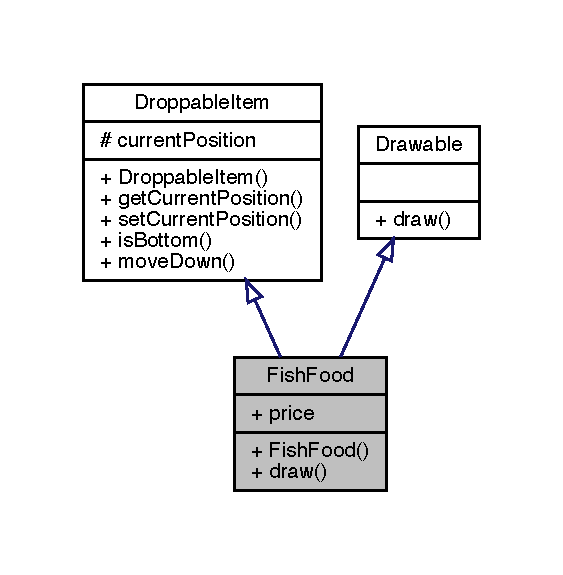
\includegraphics[width=270pt]{class_fish_food__inherit__graph}
\end{center}
\end{figure}


Collaboration diagram for Fish\+Food\+:
\nopagebreak
\begin{figure}[H]
\begin{center}
\leavevmode
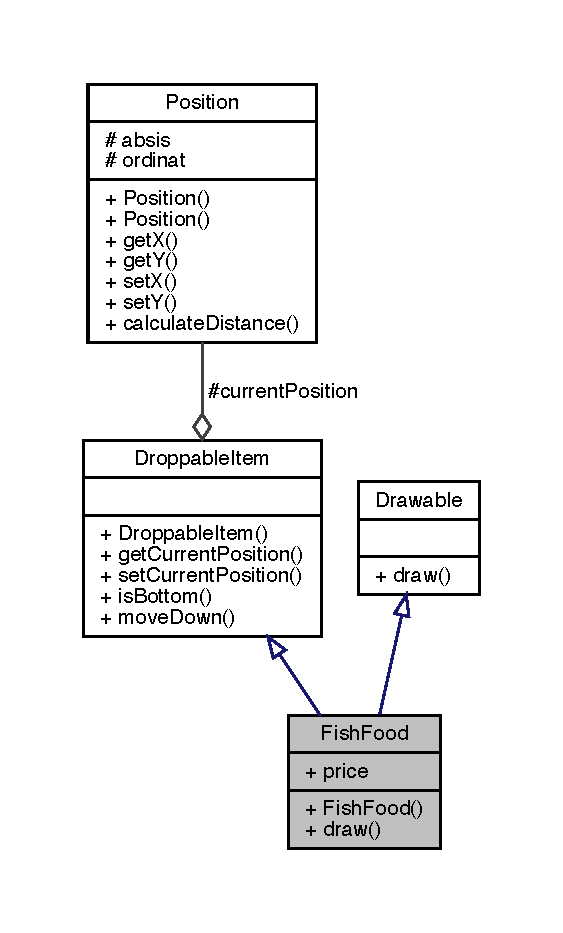
\includegraphics[width=270pt]{class_fish_food__coll__graph}
\end{center}
\end{figure}
\subsection*{Public Member Functions}
\begin{DoxyCompactItemize}
\item 
\mbox{\hyperlink{class_fish_food_a5dd9ac8ea43f95666cc95b22714e9f1c}{Fish\+Food}} (\mbox{\hyperlink{class_position}{Position}} init\+Position)
\item 
void \mbox{\hyperlink{class_fish_food_a061d353336adc633607668e8d8a73b25}{draw}} (Graphics g, Toolkit t)
\end{DoxyCompactItemize}
\subsection*{Static Public Attributes}
\begin{DoxyCompactItemize}
\item 
static final int \mbox{\hyperlink{class_fish_food_a3b3d22ebf237fb5fb445e1d8b233a777}{price}} = 10
\end{DoxyCompactItemize}
\subsection*{Additional Inherited Members}


\subsection{Detailed Description}
Represent fish food. \begin{DoxyVersion}{Version}
1.\+0. 
\end{DoxyVersion}


\subsection{Constructor \& Destructor Documentation}
\mbox{\Hypertarget{class_fish_food_a5dd9ac8ea43f95666cc95b22714e9f1c}\label{class_fish_food_a5dd9ac8ea43f95666cc95b22714e9f1c}} 
\index{Fish\+Food@{Fish\+Food}!Fish\+Food@{Fish\+Food}}
\index{Fish\+Food@{Fish\+Food}!Fish\+Food@{Fish\+Food}}
\subsubsection{\texorpdfstring{Fish\+Food()}{FishFood()}}
{\footnotesize\ttfamily Fish\+Food.\+Fish\+Food (\begin{DoxyParamCaption}\item[{\mbox{\hyperlink{class_position}{Position}}}]{init\+Position }\end{DoxyParamCaption})\hspace{0.3cm}{\ttfamily [inline]}}

constructor. 
\begin{DoxyParams}{Parameters}
{\em init\+Position} & initial position of the food. \\
\hline
\end{DoxyParams}


\subsection{Member Function Documentation}
\mbox{\Hypertarget{class_fish_food_a061d353336adc633607668e8d8a73b25}\label{class_fish_food_a061d353336adc633607668e8d8a73b25}} 
\index{Fish\+Food@{Fish\+Food}!draw@{draw}}
\index{draw@{draw}!Fish\+Food@{Fish\+Food}}
\subsubsection{\texorpdfstring{draw()}{draw()}}
{\footnotesize\ttfamily void Fish\+Food.\+draw (\begin{DoxyParamCaption}\item[{Graphics}]{g,  }\item[{Toolkit}]{t }\end{DoxyParamCaption})\hspace{0.3cm}{\ttfamily [inline]}}

draw to aquarium. 
\begin{DoxyParams}{Parameters}
{\em g} & Draw container. \\
\hline
{\em t} & Object to grab image. \\
\hline
\end{DoxyParams}


Implements \mbox{\hyperlink{interface_drawable_aaddafb212b3c8e60fcc742052570c893}{Drawable}}.

Here is the call graph for this function\+:
\nopagebreak
\begin{figure}[H]
\begin{center}
\leavevmode
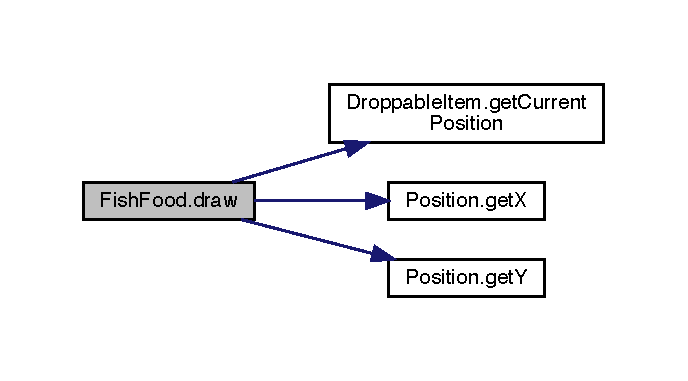
\includegraphics[width=330pt]{class_fish_food_a061d353336adc633607668e8d8a73b25_cgraph}
\end{center}
\end{figure}


\subsection{Member Data Documentation}
\mbox{\Hypertarget{class_fish_food_a3b3d22ebf237fb5fb445e1d8b233a777}\label{class_fish_food_a3b3d22ebf237fb5fb445e1d8b233a777}} 
\index{Fish\+Food@{Fish\+Food}!price@{price}}
\index{price@{price}!Fish\+Food@{Fish\+Food}}
\subsubsection{\texorpdfstring{price}{price}}
{\footnotesize\ttfamily final int Fish\+Food.\+price = 10\hspace{0.3cm}{\ttfamily [static]}}

price of fish food. 

The documentation for this class was generated from the following file\+:\begin{DoxyCompactItemize}
\item 
\mbox{\hyperlink{_fish_food_8java}{Fish\+Food.\+java}}\end{DoxyCompactItemize}

\hypertarget{class_fish_test}{}\section{Fish\+Test Class Reference}
\label{class_fish_test}\index{Fish\+Test@{Fish\+Test}}


Collaboration diagram for Fish\+Test\+:
\nopagebreak
\begin{figure}[H]
\begin{center}
\leavevmode
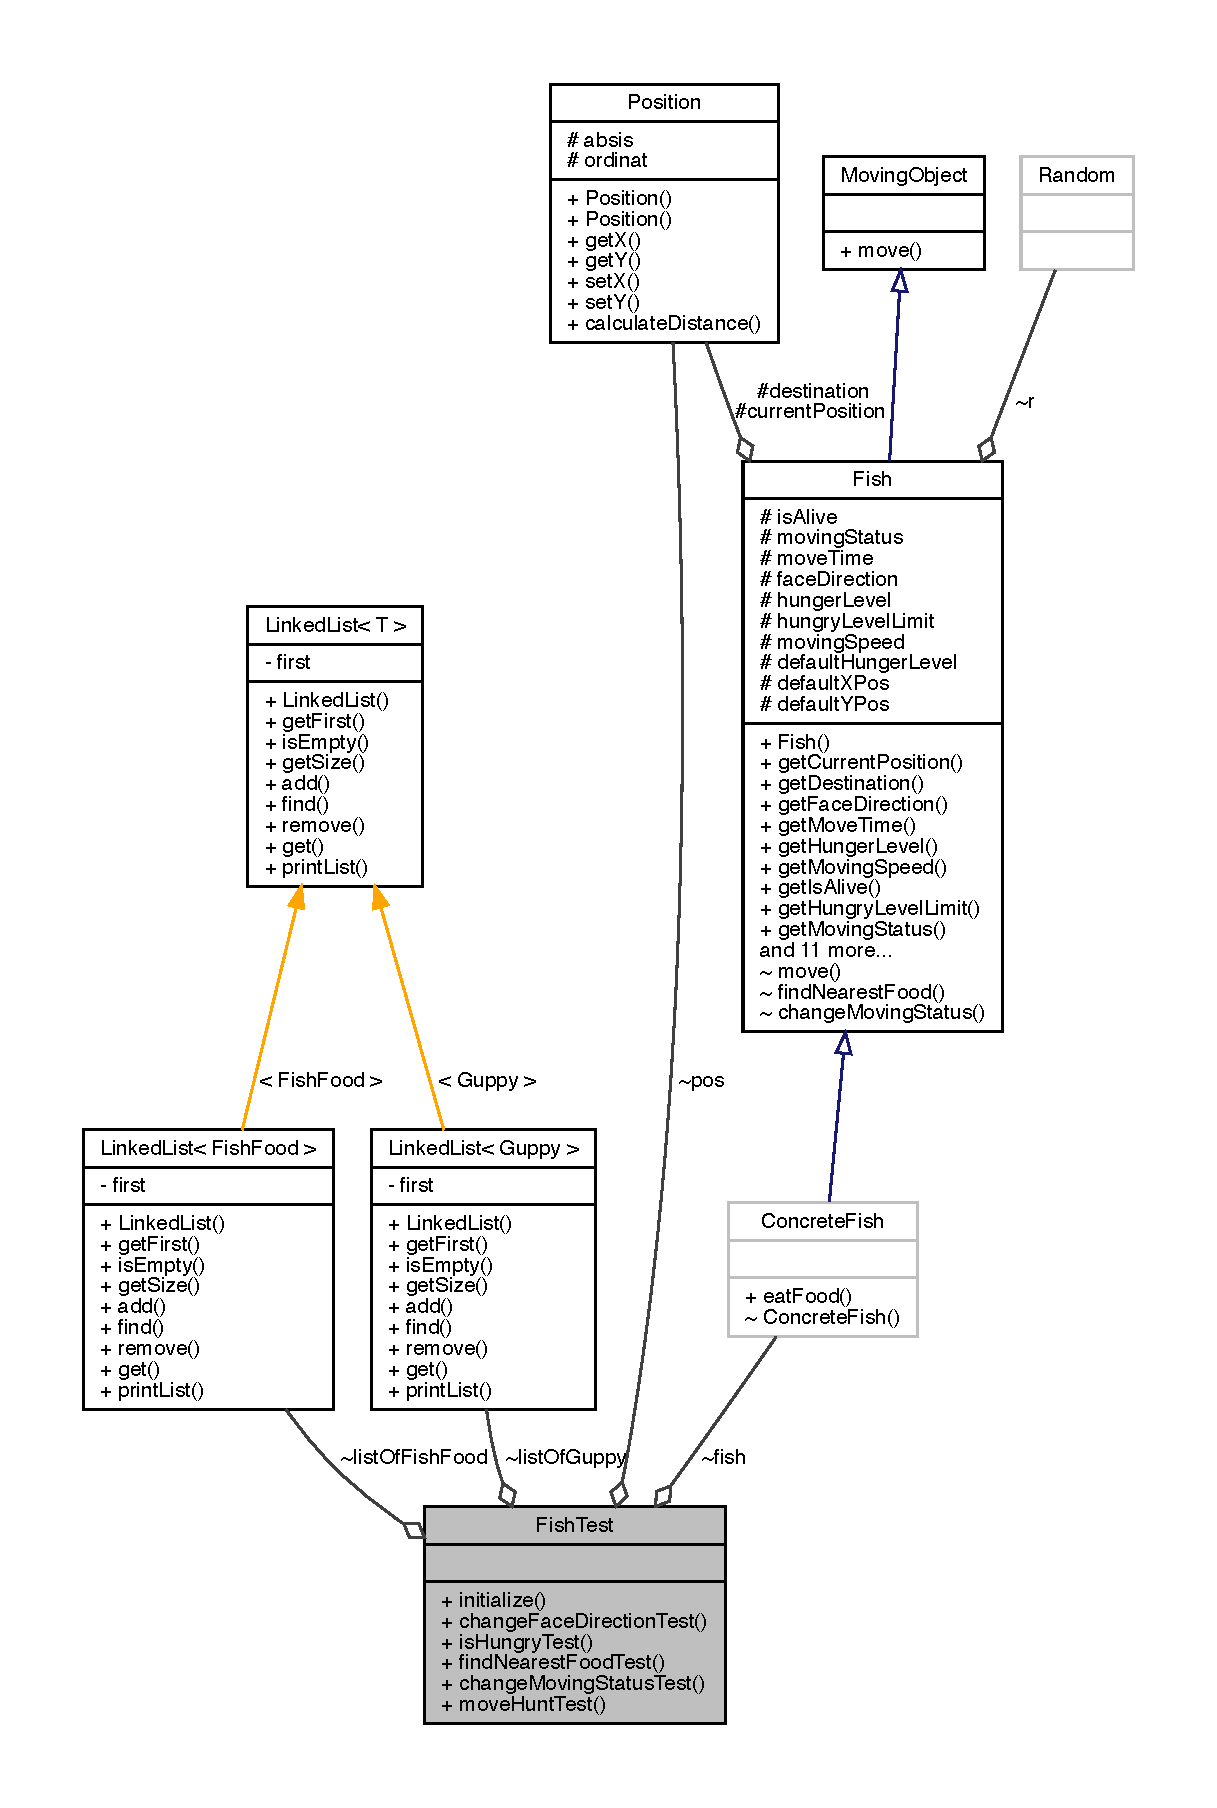
\includegraphics[width=350pt]{class_fish_test__coll__graph}
\end{center}
\end{figure}
\subsection*{Public Member Functions}
\begin{DoxyCompactItemize}
\item 
void \mbox{\hyperlink{class_fish_test_a4bc3ecb470863af45697d2dc6b7c7542}{initialize}} ()
\item 
void \mbox{\hyperlink{class_fish_test_ab32157a943c6a965e7feb4c04ffa503c}{change\+Face\+Direction\+Test}} ()
\item 
void \mbox{\hyperlink{class_fish_test_a1419dfc65a3ea1fd0c4f40a4e611320d}{is\+Hungry\+Test}} ()
\item 
void \mbox{\hyperlink{class_fish_test_af6db6a8b19fbc092877837f98576f3a8}{find\+Nearest\+Food\+Test}} ()
\item 
void \mbox{\hyperlink{class_fish_test_af7d7685db2f835899b3374243e47cc20}{change\+Moving\+Status\+Test}} ()
\item 
void \mbox{\hyperlink{class_fish_test_ac85858cd7b8d49b0490e4ef1221e3bef}{move\+Hunt\+Test}} ()
\end{DoxyCompactItemize}


\subsection{Member Function Documentation}
\mbox{\Hypertarget{class_fish_test_ab32157a943c6a965e7feb4c04ffa503c}\label{class_fish_test_ab32157a943c6a965e7feb4c04ffa503c}} 
\index{Fish\+Test@{Fish\+Test}!change\+Face\+Direction\+Test@{change\+Face\+Direction\+Test}}
\index{change\+Face\+Direction\+Test@{change\+Face\+Direction\+Test}!Fish\+Test@{Fish\+Test}}
\subsubsection{\texorpdfstring{change\+Face\+Direction\+Test()}{changeFaceDirectionTest()}}
{\footnotesize\ttfamily void Fish\+Test.\+change\+Face\+Direction\+Test (\begin{DoxyParamCaption}{ }\end{DoxyParamCaption})\hspace{0.3cm}{\ttfamily [inline]}}

\mbox{\Hypertarget{class_fish_test_af7d7685db2f835899b3374243e47cc20}\label{class_fish_test_af7d7685db2f835899b3374243e47cc20}} 
\index{Fish\+Test@{Fish\+Test}!change\+Moving\+Status\+Test@{change\+Moving\+Status\+Test}}
\index{change\+Moving\+Status\+Test@{change\+Moving\+Status\+Test}!Fish\+Test@{Fish\+Test}}
\subsubsection{\texorpdfstring{change\+Moving\+Status\+Test()}{changeMovingStatusTest()}}
{\footnotesize\ttfamily void Fish\+Test.\+change\+Moving\+Status\+Test (\begin{DoxyParamCaption}{ }\end{DoxyParamCaption})\hspace{0.3cm}{\ttfamily [inline]}}

\mbox{\Hypertarget{class_fish_test_af6db6a8b19fbc092877837f98576f3a8}\label{class_fish_test_af6db6a8b19fbc092877837f98576f3a8}} 
\index{Fish\+Test@{Fish\+Test}!find\+Nearest\+Food\+Test@{find\+Nearest\+Food\+Test}}
\index{find\+Nearest\+Food\+Test@{find\+Nearest\+Food\+Test}!Fish\+Test@{Fish\+Test}}
\subsubsection{\texorpdfstring{find\+Nearest\+Food\+Test()}{findNearestFoodTest()}}
{\footnotesize\ttfamily void Fish\+Test.\+find\+Nearest\+Food\+Test (\begin{DoxyParamCaption}{ }\end{DoxyParamCaption})\hspace{0.3cm}{\ttfamily [inline]}}

\mbox{\Hypertarget{class_fish_test_a4bc3ecb470863af45697d2dc6b7c7542}\label{class_fish_test_a4bc3ecb470863af45697d2dc6b7c7542}} 
\index{Fish\+Test@{Fish\+Test}!initialize@{initialize}}
\index{initialize@{initialize}!Fish\+Test@{Fish\+Test}}
\subsubsection{\texorpdfstring{initialize()}{initialize()}}
{\footnotesize\ttfamily void Fish\+Test.\+initialize (\begin{DoxyParamCaption}{ }\end{DoxyParamCaption})\hspace{0.3cm}{\ttfamily [inline]}}

Here is the call graph for this function\+:
\nopagebreak
\begin{figure}[H]
\begin{center}
\leavevmode
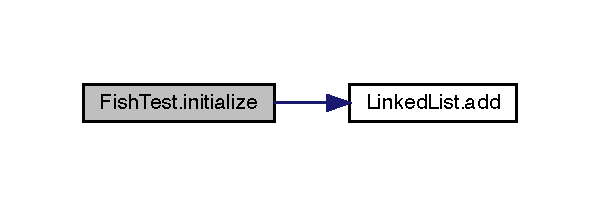
\includegraphics[width=288pt]{class_fish_test_a4bc3ecb470863af45697d2dc6b7c7542_cgraph}
\end{center}
\end{figure}
\mbox{\Hypertarget{class_fish_test_a1419dfc65a3ea1fd0c4f40a4e611320d}\label{class_fish_test_a1419dfc65a3ea1fd0c4f40a4e611320d}} 
\index{Fish\+Test@{Fish\+Test}!is\+Hungry\+Test@{is\+Hungry\+Test}}
\index{is\+Hungry\+Test@{is\+Hungry\+Test}!Fish\+Test@{Fish\+Test}}
\subsubsection{\texorpdfstring{is\+Hungry\+Test()}{isHungryTest()}}
{\footnotesize\ttfamily void Fish\+Test.\+is\+Hungry\+Test (\begin{DoxyParamCaption}{ }\end{DoxyParamCaption})\hspace{0.3cm}{\ttfamily [inline]}}

\mbox{\Hypertarget{class_fish_test_ac85858cd7b8d49b0490e4ef1221e3bef}\label{class_fish_test_ac85858cd7b8d49b0490e4ef1221e3bef}} 
\index{Fish\+Test@{Fish\+Test}!move\+Hunt\+Test@{move\+Hunt\+Test}}
\index{move\+Hunt\+Test@{move\+Hunt\+Test}!Fish\+Test@{Fish\+Test}}
\subsubsection{\texorpdfstring{move\+Hunt\+Test()}{moveHuntTest()}}
{\footnotesize\ttfamily void Fish\+Test.\+move\+Hunt\+Test (\begin{DoxyParamCaption}{ }\end{DoxyParamCaption})\hspace{0.3cm}{\ttfamily [inline]}}



The documentation for this class was generated from the following file\+:\begin{DoxyCompactItemize}
\item 
\mbox{\hyperlink{_fish_test_8java}{Fish\+Test.\+java}}\end{DoxyCompactItemize}

\hypertarget{class_guppy}{}\section{Guppy Class Reference}
\label{class_guppy}\index{Guppy@{Guppy}}


Inheritance diagram for Guppy\+:
\nopagebreak
\begin{figure}[H]
\begin{center}
\leavevmode
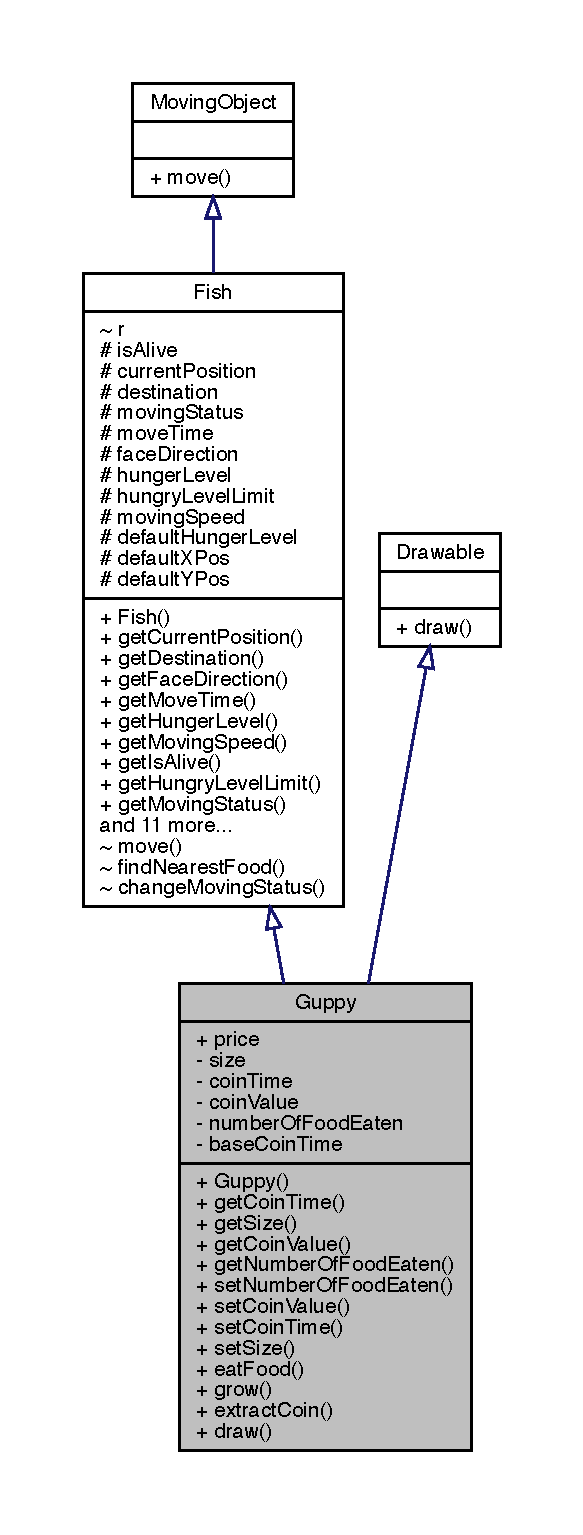
\includegraphics[height=550pt]{class_guppy__inherit__graph}
\end{center}
\end{figure}


Collaboration diagram for Guppy\+:
\nopagebreak
\begin{figure}[H]
\begin{center}
\leavevmode
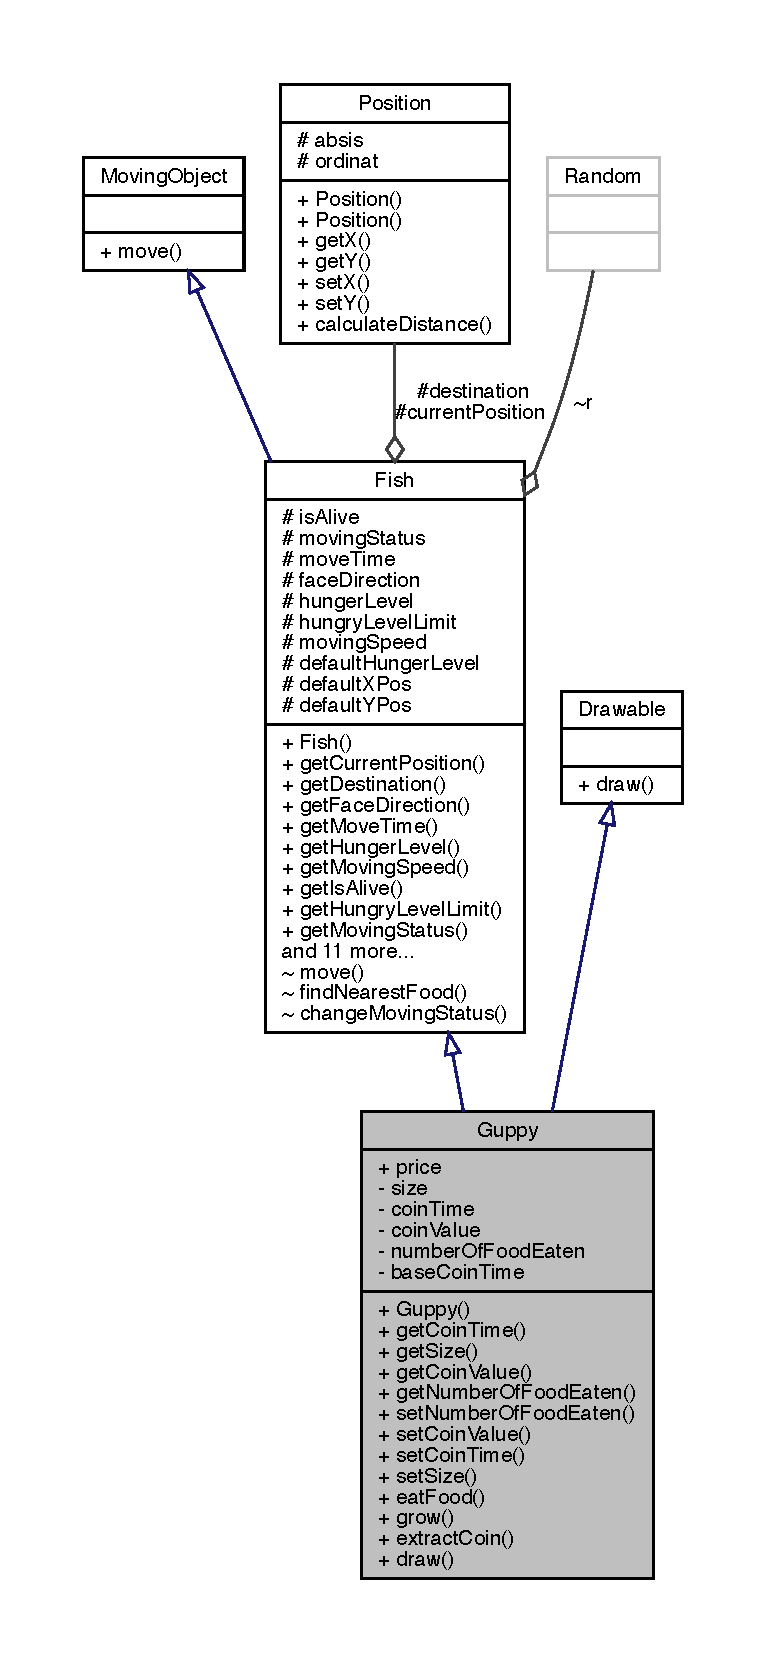
\includegraphics[height=550pt]{class_guppy__coll__graph}
\end{center}
\end{figure}
\subsection*{Public Member Functions}
\begin{DoxyCompactItemize}
\item 
\mbox{\hyperlink{class_guppy_a6336822c9cc2106fad2aaa2e54d159ac}{Guppy}} ()
\item 
double \mbox{\hyperlink{class_guppy_a7279fb164e708367a71b3d8501adff97}{get\+Coin\+Time}} ()
\item 
int \mbox{\hyperlink{class_guppy_a14ca9e79a2fe085224f240e496c9905e}{get\+Size}} ()
\item 
int \mbox{\hyperlink{class_guppy_a05b113a4bac22e8214a671da03b52294}{get\+Coin\+Value}} ()
\item 
int \mbox{\hyperlink{class_guppy_a1b4fd13a880aa51ad21dd2357e5aaa2b}{get\+Number\+Of\+Food\+Eaten}} ()
\item 
void \mbox{\hyperlink{class_guppy_a90ce9ea9c330c5d8bab256a244a995e3}{set\+Number\+Of\+Food\+Eaten}} (int \mbox{\hyperlink{class_guppy_a6a7badd3d1d55d0b02f74be82bccba59}{number\+Of\+Food\+Eaten}})
\item 
void \mbox{\hyperlink{class_guppy_a22e7cfdc2493eed638c69edee5848f2d}{set\+Coin\+Value}} (int \mbox{\hyperlink{class_guppy_aa88181b53a81e582657fce01c32090e1}{coin\+Value}})
\item 
void \mbox{\hyperlink{class_guppy_a254e1b5a56245740dcdc2c41cffaf15b}{set\+Coin\+Time}} (double \mbox{\hyperlink{class_guppy_a897004763fd0148c120166ff51650a74}{coin\+Time}})
\item 
void \mbox{\hyperlink{class_guppy_addf35bc76c2053fea12a8d0aac54d177}{set\+Size}} (int \mbox{\hyperlink{class_guppy_a2424f5424eb13aab67ee61d0876aaf25}{size}})
\item 
void \mbox{\hyperlink{class_guppy_a2b234c201f80dbed1db3a58e4ee7840b}{eat\+Food}} ()
\item 
void \mbox{\hyperlink{class_guppy_aa36c77e990d4959dc81adbe457e989c3}{grow}} ()
\item 
\mbox{\hyperlink{class_coin}{Coin}} \mbox{\hyperlink{class_guppy_aa78a5306116056c8b4bedcf79bae6ad3}{extract\+Coin}} ()
\item 
void \mbox{\hyperlink{class_guppy_ad04fab448adc11ff3eecf3a76c64781b}{draw}} (Graphics g, Toolkit t)
\end{DoxyCompactItemize}
\subsection*{Static Public Attributes}
\begin{DoxyCompactItemize}
\item 
static final int \mbox{\hyperlink{class_guppy_a711b1ce05b2a4e55af2bbab10876a56d}{price}} = 50
\end{DoxyCompactItemize}
\subsection*{Private Attributes}
\begin{DoxyCompactItemize}
\item 
int \mbox{\hyperlink{class_guppy_a2424f5424eb13aab67ee61d0876aaf25}{size}}
\item 
double \mbox{\hyperlink{class_guppy_a897004763fd0148c120166ff51650a74}{coin\+Time}}
\item 
int \mbox{\hyperlink{class_guppy_aa88181b53a81e582657fce01c32090e1}{coin\+Value}}
\item 
int \mbox{\hyperlink{class_guppy_a6a7badd3d1d55d0b02f74be82bccba59}{number\+Of\+Food\+Eaten}}
\item 
final double \mbox{\hyperlink{class_guppy_a7f87fda9dabab833cb7223c32d6d86e2}{base\+Coin\+Time}} = 15.\+0
\end{DoxyCompactItemize}
\subsection*{Additional Inherited Members}


\subsection{Detailed Description}
represent guppy. \begin{DoxyVersion}{Version}
1.\+0. 
\end{DoxyVersion}


\subsection{Constructor \& Destructor Documentation}
\mbox{\Hypertarget{class_guppy_a6336822c9cc2106fad2aaa2e54d159ac}\label{class_guppy_a6336822c9cc2106fad2aaa2e54d159ac}} 
\index{Guppy@{Guppy}!Guppy@{Guppy}}
\index{Guppy@{Guppy}!Guppy@{Guppy}}
\subsubsection{\texorpdfstring{Guppy()}{Guppy()}}
{\footnotesize\ttfamily Guppy.\+Guppy (\begin{DoxyParamCaption}{ }\end{DoxyParamCaption})\hspace{0.3cm}{\ttfamily [inline]}}

constructor. 

\subsection{Member Function Documentation}
\mbox{\Hypertarget{class_guppy_ad04fab448adc11ff3eecf3a76c64781b}\label{class_guppy_ad04fab448adc11ff3eecf3a76c64781b}} 
\index{Guppy@{Guppy}!draw@{draw}}
\index{draw@{draw}!Guppy@{Guppy}}
\subsubsection{\texorpdfstring{draw()}{draw()}}
{\footnotesize\ttfamily void Guppy.\+draw (\begin{DoxyParamCaption}\item[{Graphics}]{g,  }\item[{Toolkit}]{t }\end{DoxyParamCaption})\hspace{0.3cm}{\ttfamily [inline]}}

draw. 
\begin{DoxyParams}{Parameters}
{\em g} & Draw Container. \\
\hline
{\em t} & Object to grab image. \\
\hline
\end{DoxyParams}


Implements \mbox{\hyperlink{interface_drawable_aaddafb212b3c8e60fcc742052570c893}{Drawable}}.

Here is the call graph for this function\+:
\nopagebreak
\begin{figure}[H]
\begin{center}
\leavevmode
\includegraphics[width=306pt]{class_guppy_ad04fab448adc11ff3eecf3a76c64781b_cgraph}
\end{center}
\end{figure}
\mbox{\Hypertarget{class_guppy_a2b234c201f80dbed1db3a58e4ee7840b}\label{class_guppy_a2b234c201f80dbed1db3a58e4ee7840b}} 
\index{Guppy@{Guppy}!eat\+Food@{eat\+Food}}
\index{eat\+Food@{eat\+Food}!Guppy@{Guppy}}
\subsubsection{\texorpdfstring{eat\+Food()}{eatFood()}}
{\footnotesize\ttfamily void Guppy.\+eat\+Food (\begin{DoxyParamCaption}{ }\end{DoxyParamCaption})\hspace{0.3cm}{\ttfamily [inline]}}

eat food. Here is the call graph for this function\+:
\nopagebreak
\begin{figure}[H]
\begin{center}
\leavevmode
\includegraphics[width=269pt]{class_guppy_a2b234c201f80dbed1db3a58e4ee7840b_cgraph}
\end{center}
\end{figure}
\mbox{\Hypertarget{class_guppy_aa78a5306116056c8b4bedcf79bae6ad3}\label{class_guppy_aa78a5306116056c8b4bedcf79bae6ad3}} 
\index{Guppy@{Guppy}!extract\+Coin@{extract\+Coin}}
\index{extract\+Coin@{extract\+Coin}!Guppy@{Guppy}}
\subsubsection{\texorpdfstring{extract\+Coin()}{extractCoin()}}
{\footnotesize\ttfamily \mbox{\hyperlink{class_coin}{Coin}} Guppy.\+extract\+Coin (\begin{DoxyParamCaption}{ }\end{DoxyParamCaption})\hspace{0.3cm}{\ttfamily [inline]}}

extract coin. \begin{DoxyReturn}{Returns}
\mbox{\hyperlink{class_coin}{Coin}} object. 
\end{DoxyReturn}
Here is the call graph for this function\+:
\nopagebreak
\begin{figure}[H]
\begin{center}
\leavevmode
\includegraphics[width=335pt]{class_guppy_aa78a5306116056c8b4bedcf79bae6ad3_cgraph}
\end{center}
\end{figure}
\mbox{\Hypertarget{class_guppy_a7279fb164e708367a71b3d8501adff97}\label{class_guppy_a7279fb164e708367a71b3d8501adff97}} 
\index{Guppy@{Guppy}!get\+Coin\+Time@{get\+Coin\+Time}}
\index{get\+Coin\+Time@{get\+Coin\+Time}!Guppy@{Guppy}}
\subsubsection{\texorpdfstring{get\+Coin\+Time()}{getCoinTime()}}
{\footnotesize\ttfamily double Guppy.\+get\+Coin\+Time (\begin{DoxyParamCaption}{ }\end{DoxyParamCaption})\hspace{0.3cm}{\ttfamily [inline]}}

getter. \begin{DoxyReturn}{Returns}
double coin\+Time. 
\end{DoxyReturn}
\mbox{\Hypertarget{class_guppy_a05b113a4bac22e8214a671da03b52294}\label{class_guppy_a05b113a4bac22e8214a671da03b52294}} 
\index{Guppy@{Guppy}!get\+Coin\+Value@{get\+Coin\+Value}}
\index{get\+Coin\+Value@{get\+Coin\+Value}!Guppy@{Guppy}}
\subsubsection{\texorpdfstring{get\+Coin\+Value()}{getCoinValue()}}
{\footnotesize\ttfamily int Guppy.\+get\+Coin\+Value (\begin{DoxyParamCaption}{ }\end{DoxyParamCaption})\hspace{0.3cm}{\ttfamily [inline]}}

getter. \begin{DoxyReturn}{Returns}
integer coin value. 
\end{DoxyReturn}
\mbox{\Hypertarget{class_guppy_a1b4fd13a880aa51ad21dd2357e5aaa2b}\label{class_guppy_a1b4fd13a880aa51ad21dd2357e5aaa2b}} 
\index{Guppy@{Guppy}!get\+Number\+Of\+Food\+Eaten@{get\+Number\+Of\+Food\+Eaten}}
\index{get\+Number\+Of\+Food\+Eaten@{get\+Number\+Of\+Food\+Eaten}!Guppy@{Guppy}}
\subsubsection{\texorpdfstring{get\+Number\+Of\+Food\+Eaten()}{getNumberOfFoodEaten()}}
{\footnotesize\ttfamily int Guppy.\+get\+Number\+Of\+Food\+Eaten (\begin{DoxyParamCaption}{ }\end{DoxyParamCaption})\hspace{0.3cm}{\ttfamily [inline]}}

getter. \begin{DoxyReturn}{Returns}
integer number\+Of\+Food\+Eaten. 
\end{DoxyReturn}
\mbox{\Hypertarget{class_guppy_a14ca9e79a2fe085224f240e496c9905e}\label{class_guppy_a14ca9e79a2fe085224f240e496c9905e}} 
\index{Guppy@{Guppy}!get\+Size@{get\+Size}}
\index{get\+Size@{get\+Size}!Guppy@{Guppy}}
\subsubsection{\texorpdfstring{get\+Size()}{getSize()}}
{\footnotesize\ttfamily int Guppy.\+get\+Size (\begin{DoxyParamCaption}{ }\end{DoxyParamCaption})\hspace{0.3cm}{\ttfamily [inline]}}

getter. \begin{DoxyReturn}{Returns}
integer guppy\+Size. 
\end{DoxyReturn}
\mbox{\Hypertarget{class_guppy_aa36c77e990d4959dc81adbe457e989c3}\label{class_guppy_aa36c77e990d4959dc81adbe457e989c3}} 
\index{Guppy@{Guppy}!grow@{grow}}
\index{grow@{grow}!Guppy@{Guppy}}
\subsubsection{\texorpdfstring{grow()}{grow()}}
{\footnotesize\ttfamily void Guppy.\+grow (\begin{DoxyParamCaption}{ }\end{DoxyParamCaption})\hspace{0.3cm}{\ttfamily [inline]}}

increase guppy size. \mbox{\Hypertarget{class_guppy_a254e1b5a56245740dcdc2c41cffaf15b}\label{class_guppy_a254e1b5a56245740dcdc2c41cffaf15b}} 
\index{Guppy@{Guppy}!set\+Coin\+Time@{set\+Coin\+Time}}
\index{set\+Coin\+Time@{set\+Coin\+Time}!Guppy@{Guppy}}
\subsubsection{\texorpdfstring{set\+Coin\+Time()}{setCoinTime()}}
{\footnotesize\ttfamily void Guppy.\+set\+Coin\+Time (\begin{DoxyParamCaption}\item[{double}]{coin\+Time }\end{DoxyParamCaption})\hspace{0.3cm}{\ttfamily [inline]}}

setter. 
\begin{DoxyParams}{Parameters}
{\em coin\+Time} & double. \\
\hline
\end{DoxyParams}
\mbox{\Hypertarget{class_guppy_a22e7cfdc2493eed638c69edee5848f2d}\label{class_guppy_a22e7cfdc2493eed638c69edee5848f2d}} 
\index{Guppy@{Guppy}!set\+Coin\+Value@{set\+Coin\+Value}}
\index{set\+Coin\+Value@{set\+Coin\+Value}!Guppy@{Guppy}}
\subsubsection{\texorpdfstring{set\+Coin\+Value()}{setCoinValue()}}
{\footnotesize\ttfamily void Guppy.\+set\+Coin\+Value (\begin{DoxyParamCaption}\item[{int}]{coin\+Value }\end{DoxyParamCaption})\hspace{0.3cm}{\ttfamily [inline]}}

setter. 
\begin{DoxyParams}{Parameters}
{\em coin\+Value} & integer. \\
\hline
\end{DoxyParams}
\mbox{\Hypertarget{class_guppy_a90ce9ea9c330c5d8bab256a244a995e3}\label{class_guppy_a90ce9ea9c330c5d8bab256a244a995e3}} 
\index{Guppy@{Guppy}!set\+Number\+Of\+Food\+Eaten@{set\+Number\+Of\+Food\+Eaten}}
\index{set\+Number\+Of\+Food\+Eaten@{set\+Number\+Of\+Food\+Eaten}!Guppy@{Guppy}}
\subsubsection{\texorpdfstring{set\+Number\+Of\+Food\+Eaten()}{setNumberOfFoodEaten()}}
{\footnotesize\ttfamily void Guppy.\+set\+Number\+Of\+Food\+Eaten (\begin{DoxyParamCaption}\item[{int}]{number\+Of\+Food\+Eaten }\end{DoxyParamCaption})\hspace{0.3cm}{\ttfamily [inline]}}

setter. 
\begin{DoxyParams}{Parameters}
{\em number\+Of\+Food\+Eaten} & change number\+Of\+Food\+Eaten. \\
\hline
\end{DoxyParams}
\mbox{\Hypertarget{class_guppy_addf35bc76c2053fea12a8d0aac54d177}\label{class_guppy_addf35bc76c2053fea12a8d0aac54d177}} 
\index{Guppy@{Guppy}!set\+Size@{set\+Size}}
\index{set\+Size@{set\+Size}!Guppy@{Guppy}}
\subsubsection{\texorpdfstring{set\+Size()}{setSize()}}
{\footnotesize\ttfamily void Guppy.\+set\+Size (\begin{DoxyParamCaption}\item[{int}]{size }\end{DoxyParamCaption})\hspace{0.3cm}{\ttfamily [inline]}}

setter. 
\begin{DoxyParams}{Parameters}
{\em size} & integer. \\
\hline
\end{DoxyParams}


\subsection{Member Data Documentation}
\mbox{\Hypertarget{class_guppy_a7f87fda9dabab833cb7223c32d6d86e2}\label{class_guppy_a7f87fda9dabab833cb7223c32d6d86e2}} 
\index{Guppy@{Guppy}!base\+Coin\+Time@{base\+Coin\+Time}}
\index{base\+Coin\+Time@{base\+Coin\+Time}!Guppy@{Guppy}}
\subsubsection{\texorpdfstring{base\+Coin\+Time}{baseCoinTime}}
{\footnotesize\ttfamily final double Guppy.\+base\+Coin\+Time = 15.\+0\hspace{0.3cm}{\ttfamily [private]}}

\mbox{\Hypertarget{class_guppy_a897004763fd0148c120166ff51650a74}\label{class_guppy_a897004763fd0148c120166ff51650a74}} 
\index{Guppy@{Guppy}!coin\+Time@{coin\+Time}}
\index{coin\+Time@{coin\+Time}!Guppy@{Guppy}}
\subsubsection{\texorpdfstring{coin\+Time}{coinTime}}
{\footnotesize\ttfamily double Guppy.\+coin\+Time\hspace{0.3cm}{\ttfamily [private]}}

\mbox{\Hypertarget{class_guppy_aa88181b53a81e582657fce01c32090e1}\label{class_guppy_aa88181b53a81e582657fce01c32090e1}} 
\index{Guppy@{Guppy}!coin\+Value@{coin\+Value}}
\index{coin\+Value@{coin\+Value}!Guppy@{Guppy}}
\subsubsection{\texorpdfstring{coin\+Value}{coinValue}}
{\footnotesize\ttfamily int Guppy.\+coin\+Value\hspace{0.3cm}{\ttfamily [private]}}

\mbox{\Hypertarget{class_guppy_a6a7badd3d1d55d0b02f74be82bccba59}\label{class_guppy_a6a7badd3d1d55d0b02f74be82bccba59}} 
\index{Guppy@{Guppy}!number\+Of\+Food\+Eaten@{number\+Of\+Food\+Eaten}}
\index{number\+Of\+Food\+Eaten@{number\+Of\+Food\+Eaten}!Guppy@{Guppy}}
\subsubsection{\texorpdfstring{number\+Of\+Food\+Eaten}{numberOfFoodEaten}}
{\footnotesize\ttfamily int Guppy.\+number\+Of\+Food\+Eaten\hspace{0.3cm}{\ttfamily [private]}}

\mbox{\Hypertarget{class_guppy_a711b1ce05b2a4e55af2bbab10876a56d}\label{class_guppy_a711b1ce05b2a4e55af2bbab10876a56d}} 
\index{Guppy@{Guppy}!price@{price}}
\index{price@{price}!Guppy@{Guppy}}
\subsubsection{\texorpdfstring{price}{price}}
{\footnotesize\ttfamily final int Guppy.\+price = 50\hspace{0.3cm}{\ttfamily [static]}}

guppy price. \mbox{\Hypertarget{class_guppy_a2424f5424eb13aab67ee61d0876aaf25}\label{class_guppy_a2424f5424eb13aab67ee61d0876aaf25}} 
\index{Guppy@{Guppy}!size@{size}}
\index{size@{size}!Guppy@{Guppy}}
\subsubsection{\texorpdfstring{size}{size}}
{\footnotesize\ttfamily int Guppy.\+size\hspace{0.3cm}{\ttfamily [private]}}



The documentation for this class was generated from the following file\+:\begin{DoxyCompactItemize}
\item 
\mbox{\hyperlink{_guppy_8java}{Guppy.\+java}}\end{DoxyCompactItemize}

\hypertarget{class_guppy_test}{}\section{Guppy\+Test Class Reference}
\label{class_guppy_test}\index{Guppy\+Test@{Guppy\+Test}}


Collaboration diagram for Guppy\+Test\+:
\nopagebreak
\begin{figure}[H]
\begin{center}
\leavevmode
\includegraphics[height=550pt]{class_guppy_test__coll__graph}
\end{center}
\end{figure}
\subsection*{Public Member Functions}
\begin{DoxyCompactItemize}
\item 
void \mbox{\hyperlink{class_guppy_test_a3f926a2bb6bae5ccb6e0ded7b53bfaa7}{initialization}} ()
\item 
void \mbox{\hyperlink{class_guppy_test_ac5810161de817b76932be0c2264a0980}{eat\+Food\+Test}} ()
\item 
void \mbox{\hyperlink{class_guppy_test_aee7d947a05b64664dfdfd646325d3b8a}{grow\+Test}} ()
\item 
void \mbox{\hyperlink{class_guppy_test_a1277dd581c572d4125b0599e144f726b}{extract\+Coin\+Test}} ()
\end{DoxyCompactItemize}
\subsection*{Public Attributes}
\begin{DoxyCompactItemize}
\item 
\mbox{\hyperlink{class_guppy}{Guppy}} \mbox{\hyperlink{class_guppy_test_ad7ca1cfd1192cfc0875773b82df60bfb}{guppy}}
\end{DoxyCompactItemize}


\subsection{Member Function Documentation}
\mbox{\Hypertarget{class_guppy_test_ac5810161de817b76932be0c2264a0980}\label{class_guppy_test_ac5810161de817b76932be0c2264a0980}} 
\index{Guppy\+Test@{Guppy\+Test}!eat\+Food\+Test@{eat\+Food\+Test}}
\index{eat\+Food\+Test@{eat\+Food\+Test}!Guppy\+Test@{Guppy\+Test}}
\subsubsection{\texorpdfstring{eat\+Food\+Test()}{eatFoodTest()}}
{\footnotesize\ttfamily void Guppy\+Test.\+eat\+Food\+Test (\begin{DoxyParamCaption}{ }\end{DoxyParamCaption})\hspace{0.3cm}{\ttfamily [inline]}}

Here is the call graph for this function\+:
\nopagebreak
\begin{figure}[H]
\begin{center}
\leavevmode
\includegraphics[width=350pt]{class_guppy_test_ac5810161de817b76932be0c2264a0980_cgraph}
\end{center}
\end{figure}
\mbox{\Hypertarget{class_guppy_test_a1277dd581c572d4125b0599e144f726b}\label{class_guppy_test_a1277dd581c572d4125b0599e144f726b}} 
\index{Guppy\+Test@{Guppy\+Test}!extract\+Coin\+Test@{extract\+Coin\+Test}}
\index{extract\+Coin\+Test@{extract\+Coin\+Test}!Guppy\+Test@{Guppy\+Test}}
\subsubsection{\texorpdfstring{extract\+Coin\+Test()}{extractCoinTest()}}
{\footnotesize\ttfamily void Guppy\+Test.\+extract\+Coin\+Test (\begin{DoxyParamCaption}{ }\end{DoxyParamCaption})\hspace{0.3cm}{\ttfamily [inline]}}

Here is the call graph for this function\+:
\nopagebreak
\begin{figure}[H]
\begin{center}
\leavevmode
\includegraphics[width=350pt]{class_guppy_test_a1277dd581c572d4125b0599e144f726b_cgraph}
\end{center}
\end{figure}
\mbox{\Hypertarget{class_guppy_test_aee7d947a05b64664dfdfd646325d3b8a}\label{class_guppy_test_aee7d947a05b64664dfdfd646325d3b8a}} 
\index{Guppy\+Test@{Guppy\+Test}!grow\+Test@{grow\+Test}}
\index{grow\+Test@{grow\+Test}!Guppy\+Test@{Guppy\+Test}}
\subsubsection{\texorpdfstring{grow\+Test()}{growTest()}}
{\footnotesize\ttfamily void Guppy\+Test.\+grow\+Test (\begin{DoxyParamCaption}{ }\end{DoxyParamCaption})\hspace{0.3cm}{\ttfamily [inline]}}

Here is the call graph for this function\+:
\nopagebreak
\begin{figure}[H]
\begin{center}
\leavevmode
\includegraphics[width=303pt]{class_guppy_test_aee7d947a05b64664dfdfd646325d3b8a_cgraph}
\end{center}
\end{figure}
\mbox{\Hypertarget{class_guppy_test_a3f926a2bb6bae5ccb6e0ded7b53bfaa7}\label{class_guppy_test_a3f926a2bb6bae5ccb6e0ded7b53bfaa7}} 
\index{Guppy\+Test@{Guppy\+Test}!initialization@{initialization}}
\index{initialization@{initialization}!Guppy\+Test@{Guppy\+Test}}
\subsubsection{\texorpdfstring{initialization()}{initialization()}}
{\footnotesize\ttfamily void Guppy\+Test.\+initialization (\begin{DoxyParamCaption}{ }\end{DoxyParamCaption})\hspace{0.3cm}{\ttfamily [inline]}}



\subsection{Member Data Documentation}
\mbox{\Hypertarget{class_guppy_test_ad7ca1cfd1192cfc0875773b82df60bfb}\label{class_guppy_test_ad7ca1cfd1192cfc0875773b82df60bfb}} 
\index{Guppy\+Test@{Guppy\+Test}!guppy@{guppy}}
\index{guppy@{guppy}!Guppy\+Test@{Guppy\+Test}}
\subsubsection{\texorpdfstring{guppy}{guppy}}
{\footnotesize\ttfamily \mbox{\hyperlink{class_guppy}{Guppy}} Guppy\+Test.\+guppy}



The documentation for this class was generated from the following file\+:\begin{DoxyCompactItemize}
\item 
\mbox{\hyperlink{_guppy_test_8java}{Guppy\+Test.\+java}}\end{DoxyCompactItemize}

\hypertarget{class_linked_list}{}\section{Linked\+List$<$ T $>$ Class Template Reference}
\label{class_linked_list}\index{Linked\+List$<$ T $>$@{Linked\+List$<$ T $>$}}


Inheritance diagram for Linked\+List$<$ T $>$\+:
\nopagebreak
\begin{figure}[H]
\begin{center}
\leavevmode
\includegraphics[width=350pt]{class_linked_list__inherit__graph}
\end{center}
\end{figure}


Collaboration diagram for Linked\+List$<$ T $>$\+:
\nopagebreak
\begin{figure}[H]
\begin{center}
\leavevmode
\includegraphics[width=164pt]{class_linked_list__coll__graph}
\end{center}
\end{figure}
\subsection*{Public Member Functions}
\begin{DoxyCompactItemize}
\item 
\mbox{\hyperlink{class_linked_list_ae04bfb6ff80214a33132ba72ceb117aa}{Linked\+List}} ()
\item 
Node$<$ T $>$ \mbox{\hyperlink{class_linked_list_a97e865343f67ed5879567bfb1d362a19}{get\+First}} ()
\item 
boolean \mbox{\hyperlink{class_linked_list_aecae3d82587c52087a4f65d6c56900e2}{is\+Empty}} ()
\item 
int \mbox{\hyperlink{class_linked_list_a7ea3fa6fa5601039076c2a6c8fe88219}{get\+Size}} ()
\item 
void \mbox{\hyperlink{class_linked_list_af7ec408e2f1040643d77f614af535988}{add}} (T element)
\item 
int \mbox{\hyperlink{class_linked_list_abb5fc485a297b815daf6034f1c455979}{find}} (T element)
\item 
void \mbox{\hyperlink{class_linked_list_a85388ca2d7e4c8bc06fbea2c6fcfea33}{remove}} (T element)
\item 
T \mbox{\hyperlink{class_linked_list_a032ef46fc54f12525746d9f7c3a80663}{get}} (int index)
\item 
void \mbox{\hyperlink{class_linked_list_aaa02d6cede50240f57de8115fbbc5b4d}{print\+List}} ()
\end{DoxyCompactItemize}
\subsection*{Private Attributes}
\begin{DoxyCompactItemize}
\item 
Node$<$ T $>$ \mbox{\hyperlink{class_linked_list_a34f1f7a8bd8fd70f2131b2e82f58cb32}{first}}
\end{DoxyCompactItemize}


\subsection{Detailed Description}
Represents a linkedlist \begin{DoxyVersion}{Version}
1.\+0 
\end{DoxyVersion}


\subsection{Constructor \& Destructor Documentation}
\mbox{\Hypertarget{class_linked_list_ae04bfb6ff80214a33132ba72ceb117aa}\label{class_linked_list_ae04bfb6ff80214a33132ba72ceb117aa}} 
\index{Linked\+List@{Linked\+List}!Linked\+List@{Linked\+List}}
\index{Linked\+List@{Linked\+List}!Linked\+List@{Linked\+List}}
\subsubsection{\texorpdfstring{Linked\+List()}{LinkedList()}}
{\footnotesize\ttfamily \mbox{\hyperlink{class_linked_list}{Linked\+List}}$<$ T $>$.\mbox{\hyperlink{class_linked_list}{Linked\+List}} (\begin{DoxyParamCaption}{ }\end{DoxyParamCaption})\hspace{0.3cm}{\ttfamily [inline]}}

constructor. 

\subsection{Member Function Documentation}
\mbox{\Hypertarget{class_linked_list_af7ec408e2f1040643d77f614af535988}\label{class_linked_list_af7ec408e2f1040643d77f614af535988}} 
\index{Linked\+List@{Linked\+List}!add@{add}}
\index{add@{add}!Linked\+List@{Linked\+List}}
\subsubsection{\texorpdfstring{add()}{add()}}
{\footnotesize\ttfamily void \mbox{\hyperlink{class_linked_list}{Linked\+List}}$<$ T $>$.add (\begin{DoxyParamCaption}\item[{T}]{element }\end{DoxyParamCaption})\hspace{0.3cm}{\ttfamily [inline]}}

Add to last element of linkedlist. 
\begin{DoxyParams}{Parameters}
{\em element} & element to add. \\
\hline
\end{DoxyParams}
\mbox{\Hypertarget{class_linked_list_abb5fc485a297b815daf6034f1c455979}\label{class_linked_list_abb5fc485a297b815daf6034f1c455979}} 
\index{Linked\+List@{Linked\+List}!find@{find}}
\index{find@{find}!Linked\+List@{Linked\+List}}
\subsubsection{\texorpdfstring{find()}{find()}}
{\footnotesize\ttfamily int \mbox{\hyperlink{class_linked_list}{Linked\+List}}$<$ T $>$.find (\begin{DoxyParamCaption}\item[{T}]{element }\end{DoxyParamCaption})\hspace{0.3cm}{\ttfamily [inline]}}

return index of element, or -\/1 if not available. 
\begin{DoxyParams}{Parameters}
{\em element} & element to find. \\
\hline
\end{DoxyParams}
\begin{DoxyReturn}{Returns}
integer index of the specified element. 
\end{DoxyReturn}
\mbox{\Hypertarget{class_linked_list_a032ef46fc54f12525746d9f7c3a80663}\label{class_linked_list_a032ef46fc54f12525746d9f7c3a80663}} 
\index{Linked\+List@{Linked\+List}!get@{get}}
\index{get@{get}!Linked\+List@{Linked\+List}}
\subsubsection{\texorpdfstring{get()}{get()}}
{\footnotesize\ttfamily T \mbox{\hyperlink{class_linked_list}{Linked\+List}}$<$ T $>$.get (\begin{DoxyParamCaption}\item[{int}]{index }\end{DoxyParamCaption})\hspace{0.3cm}{\ttfamily [inline]}}

get element on index, if not available return null. 
\begin{DoxyParams}{Parameters}
{\em index} & of the element. \\
\hline
\end{DoxyParams}
\begin{DoxyReturn}{Returns}
type of the element. 
\end{DoxyReturn}
\mbox{\Hypertarget{class_linked_list_a97e865343f67ed5879567bfb1d362a19}\label{class_linked_list_a97e865343f67ed5879567bfb1d362a19}} 
\index{Linked\+List@{Linked\+List}!get\+First@{get\+First}}
\index{get\+First@{get\+First}!Linked\+List@{Linked\+List}}
\subsubsection{\texorpdfstring{get\+First()}{getFirst()}}
{\footnotesize\ttfamily Node$<$T$>$ \mbox{\hyperlink{class_linked_list}{Linked\+List}}$<$ T $>$.get\+First (\begin{DoxyParamCaption}{ }\end{DoxyParamCaption})\hspace{0.3cm}{\ttfamily [inline]}}

getter. \begin{DoxyReturn}{Returns}
Node. 
\end{DoxyReturn}
\mbox{\Hypertarget{class_linked_list_a7ea3fa6fa5601039076c2a6c8fe88219}\label{class_linked_list_a7ea3fa6fa5601039076c2a6c8fe88219}} 
\index{Linked\+List@{Linked\+List}!get\+Size@{get\+Size}}
\index{get\+Size@{get\+Size}!Linked\+List@{Linked\+List}}
\subsubsection{\texorpdfstring{get\+Size()}{getSize()}}
{\footnotesize\ttfamily int \mbox{\hyperlink{class_linked_list}{Linked\+List}}$<$ T $>$.get\+Size (\begin{DoxyParamCaption}{ }\end{DoxyParamCaption})\hspace{0.3cm}{\ttfamily [inline]}}

getter. \begin{DoxyReturn}{Returns}
integer. 
\end{DoxyReturn}
\mbox{\Hypertarget{class_linked_list_aecae3d82587c52087a4f65d6c56900e2}\label{class_linked_list_aecae3d82587c52087a4f65d6c56900e2}} 
\index{Linked\+List@{Linked\+List}!is\+Empty@{is\+Empty}}
\index{is\+Empty@{is\+Empty}!Linked\+List@{Linked\+List}}
\subsubsection{\texorpdfstring{is\+Empty()}{isEmpty()}}
{\footnotesize\ttfamily boolean \mbox{\hyperlink{class_linked_list}{Linked\+List}}$<$ T $>$.is\+Empty (\begin{DoxyParamCaption}{ }\end{DoxyParamCaption})\hspace{0.3cm}{\ttfamily [inline]}}

getter. \begin{DoxyReturn}{Returns}
boolean. 
\end{DoxyReturn}
\mbox{\Hypertarget{class_linked_list_aaa02d6cede50240f57de8115fbbc5b4d}\label{class_linked_list_aaa02d6cede50240f57de8115fbbc5b4d}} 
\index{Linked\+List@{Linked\+List}!print\+List@{print\+List}}
\index{print\+List@{print\+List}!Linked\+List@{Linked\+List}}
\subsubsection{\texorpdfstring{print\+List()}{printList()}}
{\footnotesize\ttfamily void \mbox{\hyperlink{class_linked_list}{Linked\+List}}$<$ T $>$.print\+List (\begin{DoxyParamCaption}{ }\end{DoxyParamCaption})\hspace{0.3cm}{\ttfamily [inline]}}

print element in linkedlist. \mbox{\Hypertarget{class_linked_list_a85388ca2d7e4c8bc06fbea2c6fcfea33}\label{class_linked_list_a85388ca2d7e4c8bc06fbea2c6fcfea33}} 
\index{Linked\+List@{Linked\+List}!remove@{remove}}
\index{remove@{remove}!Linked\+List@{Linked\+List}}
\subsubsection{\texorpdfstring{remove()}{remove()}}
{\footnotesize\ttfamily void \mbox{\hyperlink{class_linked_list}{Linked\+List}}$<$ T $>$.remove (\begin{DoxyParamCaption}\item[{T}]{element }\end{DoxyParamCaption})\hspace{0.3cm}{\ttfamily [inline]}}

remove element from linkedlist. 
\begin{DoxyParams}{Parameters}
{\em element} & element to remove. \\
\hline
\end{DoxyParams}


\subsection{Member Data Documentation}
\mbox{\Hypertarget{class_linked_list_a34f1f7a8bd8fd70f2131b2e82f58cb32}\label{class_linked_list_a34f1f7a8bd8fd70f2131b2e82f58cb32}} 
\index{Linked\+List@{Linked\+List}!first@{first}}
\index{first@{first}!Linked\+List@{Linked\+List}}
\subsubsection{\texorpdfstring{first}{first}}
{\footnotesize\ttfamily Node$<$T$>$ \mbox{\hyperlink{class_linked_list}{Linked\+List}}$<$ T $>$.first\hspace{0.3cm}{\ttfamily [private]}}



The documentation for this class was generated from the following file\+:\begin{DoxyCompactItemize}
\item 
\mbox{\hyperlink{_linked_list_8java}{Linked\+List.\+java}}\end{DoxyCompactItemize}

\hypertarget{class_linked_list_test}{}\section{Linked\+List\+Test Class Reference}
\label{class_linked_list_test}\index{Linked\+List\+Test@{Linked\+List\+Test}}


Collaboration diagram for Linked\+List\+Test\+:
\nopagebreak
\begin{figure}[H]
\begin{center}
\leavevmode
\includegraphics[width=189pt]{class_linked_list_test__coll__graph}
\end{center}
\end{figure}
\subsection*{Public Member Functions}
\begin{DoxyCompactItemize}
\item 
void \mbox{\hyperlink{class_linked_list_test_aa351eea543f28f3246130b6d11495032}{get\+Size\+Test}} ()
\item 
void \mbox{\hyperlink{class_linked_list_test_ace2ec9faf414e71b82c0f90bcd05101c}{add\+Test}} ()
\item 
void \mbox{\hyperlink{class_linked_list_test_a7ec3ac010e6a30800f558fd8ba3963c1}{find\+Test}} ()
\item 
void \mbox{\hyperlink{class_linked_list_test_ad80814e7e3e8452c19b236fb070ee405}{remove\+Test}} ()
\item 
void \mbox{\hyperlink{class_linked_list_test_a8f9041662d2c4a40641ae02627ea3bcd}{get\+Test}} ()
\end{DoxyCompactItemize}


\subsection{Member Function Documentation}
\mbox{\Hypertarget{class_linked_list_test_ace2ec9faf414e71b82c0f90bcd05101c}\label{class_linked_list_test_ace2ec9faf414e71b82c0f90bcd05101c}} 
\index{Linked\+List\+Test@{Linked\+List\+Test}!add\+Test@{add\+Test}}
\index{add\+Test@{add\+Test}!Linked\+List\+Test@{Linked\+List\+Test}}
\subsubsection{\texorpdfstring{add\+Test()}{addTest()}}
{\footnotesize\ttfamily void Linked\+List\+Test.\+add\+Test (\begin{DoxyParamCaption}{ }\end{DoxyParamCaption})\hspace{0.3cm}{\ttfamily [inline]}}

Here is the call graph for this function\+:
\nopagebreak
\begin{figure}[H]
\begin{center}
\leavevmode
\includegraphics[width=314pt]{class_linked_list_test_ace2ec9faf414e71b82c0f90bcd05101c_cgraph}
\end{center}
\end{figure}
\mbox{\Hypertarget{class_linked_list_test_a7ec3ac010e6a30800f558fd8ba3963c1}\label{class_linked_list_test_a7ec3ac010e6a30800f558fd8ba3963c1}} 
\index{Linked\+List\+Test@{Linked\+List\+Test}!find\+Test@{find\+Test}}
\index{find\+Test@{find\+Test}!Linked\+List\+Test@{Linked\+List\+Test}}
\subsubsection{\texorpdfstring{find\+Test()}{findTest()}}
{\footnotesize\ttfamily void Linked\+List\+Test.\+find\+Test (\begin{DoxyParamCaption}{ }\end{DoxyParamCaption})\hspace{0.3cm}{\ttfamily [inline]}}

Here is the call graph for this function\+:
\nopagebreak
\begin{figure}[H]
\begin{center}
\leavevmode
\includegraphics[width=313pt]{class_linked_list_test_a7ec3ac010e6a30800f558fd8ba3963c1_cgraph}
\end{center}
\end{figure}
\mbox{\Hypertarget{class_linked_list_test_aa351eea543f28f3246130b6d11495032}\label{class_linked_list_test_aa351eea543f28f3246130b6d11495032}} 
\index{Linked\+List\+Test@{Linked\+List\+Test}!get\+Size\+Test@{get\+Size\+Test}}
\index{get\+Size\+Test@{get\+Size\+Test}!Linked\+List\+Test@{Linked\+List\+Test}}
\subsubsection{\texorpdfstring{get\+Size\+Test()}{getSizeTest()}}
{\footnotesize\ttfamily void Linked\+List\+Test.\+get\+Size\+Test (\begin{DoxyParamCaption}{ }\end{DoxyParamCaption})\hspace{0.3cm}{\ttfamily [inline]}}

Here is the call graph for this function\+:
\nopagebreak
\begin{figure}[H]
\begin{center}
\leavevmode
\includegraphics[width=347pt]{class_linked_list_test_aa351eea543f28f3246130b6d11495032_cgraph}
\end{center}
\end{figure}
\mbox{\Hypertarget{class_linked_list_test_a8f9041662d2c4a40641ae02627ea3bcd}\label{class_linked_list_test_a8f9041662d2c4a40641ae02627ea3bcd}} 
\index{Linked\+List\+Test@{Linked\+List\+Test}!get\+Test@{get\+Test}}
\index{get\+Test@{get\+Test}!Linked\+List\+Test@{Linked\+List\+Test}}
\subsubsection{\texorpdfstring{get\+Test()}{getTest()}}
{\footnotesize\ttfamily void Linked\+List\+Test.\+get\+Test (\begin{DoxyParamCaption}{ }\end{DoxyParamCaption})\hspace{0.3cm}{\ttfamily [inline]}}

Here is the call graph for this function\+:
\nopagebreak
\begin{figure}[H]
\begin{center}
\leavevmode
\includegraphics[width=311pt]{class_linked_list_test_a8f9041662d2c4a40641ae02627ea3bcd_cgraph}
\end{center}
\end{figure}
\mbox{\Hypertarget{class_linked_list_test_ad80814e7e3e8452c19b236fb070ee405}\label{class_linked_list_test_ad80814e7e3e8452c19b236fb070ee405}} 
\index{Linked\+List\+Test@{Linked\+List\+Test}!remove\+Test@{remove\+Test}}
\index{remove\+Test@{remove\+Test}!Linked\+List\+Test@{Linked\+List\+Test}}
\subsubsection{\texorpdfstring{remove\+Test()}{removeTest()}}
{\footnotesize\ttfamily void Linked\+List\+Test.\+remove\+Test (\begin{DoxyParamCaption}{ }\end{DoxyParamCaption})\hspace{0.3cm}{\ttfamily [inline]}}

Here is the call graph for this function\+:
\nopagebreak
\begin{figure}[H]
\begin{center}
\leavevmode
\includegraphics[width=347pt]{class_linked_list_test_ad80814e7e3e8452c19b236fb070ee405_cgraph}
\end{center}
\end{figure}


The documentation for this class was generated from the following file\+:\begin{DoxyCompactItemize}
\item 
\mbox{\hyperlink{_linked_list_test_8java}{Linked\+List\+Test.\+java}}\end{DoxyCompactItemize}

\hypertarget{class_main}{}\section{Main Class Reference}
\label{class_main}\index{Main@{Main}}


Collaboration diagram for Main\+:
\nopagebreak
\begin{figure}[H]
\begin{center}
\leavevmode
\includegraphics[width=133pt]{class_main__coll__graph}
\end{center}
\end{figure}
\subsection*{Static Public Member Functions}
\begin{DoxyCompactItemize}
\item 
static void \mbox{\hyperlink{class_main_a8a5d0f827edddff706cc0e6740d0579a}{main}} (String\mbox{[}$\,$\mbox{]} args)
\end{DoxyCompactItemize}


\subsection{Detailed Description}
main program \begin{DoxyVersion}{Version}
1.\+0 
\end{DoxyVersion}


\subsection{Member Function Documentation}
\mbox{\Hypertarget{class_main_a8a5d0f827edddff706cc0e6740d0579a}\label{class_main_a8a5d0f827edddff706cc0e6740d0579a}} 
\index{Main@{Main}!main@{main}}
\index{main@{main}!Main@{Main}}
\subsubsection{\texorpdfstring{main()}{main()}}
{\footnotesize\ttfamily static void Main.\+main (\begin{DoxyParamCaption}\item[{String \mbox{[}$\,$\mbox{]}}]{args }\end{DoxyParamCaption})\hspace{0.3cm}{\ttfamily [inline]}, {\ttfamily [static]}}

run. Here is the call graph for this function\+:
\nopagebreak
\begin{figure}[H]
\begin{center}
\leavevmode
\includegraphics[width=350pt]{class_main_a8a5d0f827edddff706cc0e6740d0579a_cgraph}
\end{center}
\end{figure}


The documentation for this class was generated from the following file\+:\begin{DoxyCompactItemize}
\item 
\mbox{\hyperlink{_main_8java}{Main.\+java}}\end{DoxyCompactItemize}

\hypertarget{interface_moving_object}{}\section{Moving\+Object Interface Reference}
\label{interface_moving_object}\index{Moving\+Object@{Moving\+Object}}


Inheritance diagram for Moving\+Object\+:
\nopagebreak
\begin{figure}[H]
\begin{center}
\leavevmode
\includegraphics[height=550pt]{interface_moving_object__inherit__graph}
\end{center}
\end{figure}


Collaboration diagram for Moving\+Object\+:
\nopagebreak
\begin{figure}[H]
\begin{center}
\leavevmode
\includegraphics[width=157pt]{interface_moving_object__coll__graph}
\end{center}
\end{figure}
\subsection*{Classes}
\begin{DoxyCompactItemize}
\item 
enum \mbox{\hyperlink{enum_moving_object_1_1_moving_status}{Moving\+Status}}
\end{DoxyCompactItemize}
\subsection*{Public Member Functions}
\begin{DoxyCompactItemize}
\item 
public$<$ T $>$ void \mbox{\hyperlink{interface_moving_object_a1e3f8b0a047bb3db15f64263ca4ea464}{move}} (\mbox{\hyperlink{class_linked_list}{Linked\+List}}$<$ T $>$ food)
\end{DoxyCompactItemize}


\subsection{Detailed Description}
moving object interface. \begin{DoxyVersion}{Version}
1.\+0. 
\end{DoxyVersion}


\subsection{Member Function Documentation}
\mbox{\Hypertarget{interface_moving_object_a1e3f8b0a047bb3db15f64263ca4ea464}\label{interface_moving_object_a1e3f8b0a047bb3db15f64263ca4ea464}} 
\index{Moving\+Object@{Moving\+Object}!move@{move}}
\index{move@{move}!Moving\+Object@{Moving\+Object}}
\subsubsection{\texorpdfstring{move()}{move()}}
{\footnotesize\ttfamily public$<$T$>$ void Moving\+Object.\+move (\begin{DoxyParamCaption}\item[{\mbox{\hyperlink{class_linked_list}{Linked\+List}}$<$ T $>$}]{food }\end{DoxyParamCaption})}

move. 
\begin{DoxyParams}{Parameters}
{\em food} & \mbox{\hyperlink{class_linked_list}{Linked\+List}} of food. \\
\hline
\end{DoxyParams}


The documentation for this interface was generated from the following file\+:\begin{DoxyCompactItemize}
\item 
\mbox{\hyperlink{_moving_object_8java}{Moving\+Object.\+java}}\end{DoxyCompactItemize}

\hypertarget{enum_moving_object_1_1_moving_status}{}\section{Moving\+Object.\+Moving\+Status Enum Reference}
\label{enum_moving_object_1_1_moving_status}\index{Moving\+Object.\+Moving\+Status@{Moving\+Object.\+Moving\+Status}}


Collaboration diagram for Moving\+Object.\+Moving\+Status\+:
\nopagebreak
\begin{figure}[H]
\begin{center}
\leavevmode
\includegraphics[width=221pt]{enum_moving_object_1_1_moving_status__coll__graph}
\end{center}
\end{figure}
\subsection*{Public Attributes}
\begin{DoxyCompactItemize}
\item 
\mbox{\hyperlink{enum_moving_object_1_1_moving_status_ab46cd9780091a74038f2bba2e15998d7}{R\+A\+N\+D\+OM}}
\item 
\mbox{\hyperlink{enum_moving_object_1_1_moving_status_ad37d0a6b5268276a61c3a4373829f96c}{H\+U\+N\+T\+I\+NG}}
\end{DoxyCompactItemize}


\subsection{Detailed Description}
enum. 

\subsection{Member Data Documentation}
\mbox{\Hypertarget{enum_moving_object_1_1_moving_status_ad37d0a6b5268276a61c3a4373829f96c}\label{enum_moving_object_1_1_moving_status_ad37d0a6b5268276a61c3a4373829f96c}} 
\index{Moving\+Object\+::\+Moving\+Status@{Moving\+Object\+::\+Moving\+Status}!H\+U\+N\+T\+I\+NG@{H\+U\+N\+T\+I\+NG}}
\index{H\+U\+N\+T\+I\+NG@{H\+U\+N\+T\+I\+NG}!Moving\+Object\+::\+Moving\+Status@{Moving\+Object\+::\+Moving\+Status}}
\subsubsection{\texorpdfstring{H\+U\+N\+T\+I\+NG}{HUNTING}}
{\footnotesize\ttfamily Moving\+Object.\+Moving\+Status.\+H\+U\+N\+T\+I\+NG}

\mbox{\Hypertarget{enum_moving_object_1_1_moving_status_ab46cd9780091a74038f2bba2e15998d7}\label{enum_moving_object_1_1_moving_status_ab46cd9780091a74038f2bba2e15998d7}} 
\index{Moving\+Object\+::\+Moving\+Status@{Moving\+Object\+::\+Moving\+Status}!R\+A\+N\+D\+OM@{R\+A\+N\+D\+OM}}
\index{R\+A\+N\+D\+OM@{R\+A\+N\+D\+OM}!Moving\+Object\+::\+Moving\+Status@{Moving\+Object\+::\+Moving\+Status}}
\subsubsection{\texorpdfstring{R\+A\+N\+D\+OM}{RANDOM}}
{\footnotesize\ttfamily Moving\+Object.\+Moving\+Status.\+R\+A\+N\+D\+OM}



The documentation for this enum was generated from the following file\+:\begin{DoxyCompactItemize}
\item 
\mbox{\hyperlink{_moving_object_8java}{Moving\+Object.\+java}}\end{DoxyCompactItemize}

\hypertarget{class_piranha}{}\section{Piranha Class Reference}
\label{class_piranha}\index{Piranha@{Piranha}}


Inheritance diagram for Piranha\+:
\nopagebreak
\begin{figure}[H]
\begin{center}
\leavevmode
\includegraphics[height=550pt]{class_piranha__inherit__graph}
\end{center}
\end{figure}


Collaboration diagram for Piranha\+:
\nopagebreak
\begin{figure}[H]
\begin{center}
\leavevmode
\includegraphics[height=550pt]{class_piranha__coll__graph}
\end{center}
\end{figure}
\subsection*{Public Member Functions}
\begin{DoxyCompactItemize}
\item 
\mbox{\hyperlink{class_piranha_a162bfb763ec65582d2631cb44905b8b0}{Piranha}} ()
\item 
\mbox{\hyperlink{class_coin}{Coin}} \mbox{\hyperlink{class_piranha_a2cf10bd7477bf06d0f5020411acfe95d}{extract\+Coin}} (int val)
\item 
void \mbox{\hyperlink{class_piranha_a9310ca27aa9c8fdec55f03ef4fa994e0}{eat\+Food}} ()
\item 
void \mbox{\hyperlink{class_piranha_a8a06429a9c5b42fb4246f48c54d6cf78}{draw}} (Graphics g, Toolkit t)
\end{DoxyCompactItemize}
\subsection*{Static Public Attributes}
\begin{DoxyCompactItemize}
\item 
static final int \mbox{\hyperlink{class_piranha_a4df74b901061840159a8b8e0d5e14f88}{price}} = 100
\end{DoxyCompactItemize}
\subsection*{Additional Inherited Members}


\subsection{Detailed Description}
represents a \mbox{\hyperlink{class_piranha}{Piranha}}. \begin{DoxyVersion}{Version}
1.\+0. 
\end{DoxyVersion}


\subsection{Constructor \& Destructor Documentation}
\mbox{\Hypertarget{class_piranha_a162bfb763ec65582d2631cb44905b8b0}\label{class_piranha_a162bfb763ec65582d2631cb44905b8b0}} 
\index{Piranha@{Piranha}!Piranha@{Piranha}}
\index{Piranha@{Piranha}!Piranha@{Piranha}}
\subsubsection{\texorpdfstring{Piranha()}{Piranha()}}
{\footnotesize\ttfamily Piranha.\+Piranha (\begin{DoxyParamCaption}{ }\end{DoxyParamCaption})\hspace{0.3cm}{\ttfamily [inline]}}

constructor. 

\subsection{Member Function Documentation}
\mbox{\Hypertarget{class_piranha_a8a06429a9c5b42fb4246f48c54d6cf78}\label{class_piranha_a8a06429a9c5b42fb4246f48c54d6cf78}} 
\index{Piranha@{Piranha}!draw@{draw}}
\index{draw@{draw}!Piranha@{Piranha}}
\subsubsection{\texorpdfstring{draw()}{draw()}}
{\footnotesize\ttfamily void Piranha.\+draw (\begin{DoxyParamCaption}\item[{Graphics}]{g,  }\item[{Toolkit}]{t }\end{DoxyParamCaption})\hspace{0.3cm}{\ttfamily [inline]}}

draw to aquarium. 
\begin{DoxyParams}{Parameters}
{\em g} & Draw container. \\
\hline
{\em t} & Object to grab image. \\
\hline
\end{DoxyParams}


Implements \mbox{\hyperlink{interface_drawable_aaddafb212b3c8e60fcc742052570c893}{Drawable}}.

Here is the call graph for this function\+:
\nopagebreak
\begin{figure}[H]
\begin{center}
\leavevmode
\includegraphics[width=311pt]{class_piranha_a8a06429a9c5b42fb4246f48c54d6cf78_cgraph}
\end{center}
\end{figure}
\mbox{\Hypertarget{class_piranha_a9310ca27aa9c8fdec55f03ef4fa994e0}\label{class_piranha_a9310ca27aa9c8fdec55f03ef4fa994e0}} 
\index{Piranha@{Piranha}!eat\+Food@{eat\+Food}}
\index{eat\+Food@{eat\+Food}!Piranha@{Piranha}}
\subsubsection{\texorpdfstring{eat\+Food()}{eatFood()}}
{\footnotesize\ttfamily void Piranha.\+eat\+Food (\begin{DoxyParamCaption}{ }\end{DoxyParamCaption})\hspace{0.3cm}{\ttfamily [inline]}}

eat food. Here is the call graph for this function\+:
\nopagebreak
\begin{figure}[H]
\begin{center}
\leavevmode
\includegraphics[width=314pt]{class_piranha_a9310ca27aa9c8fdec55f03ef4fa994e0_cgraph}
\end{center}
\end{figure}
\mbox{\Hypertarget{class_piranha_a2cf10bd7477bf06d0f5020411acfe95d}\label{class_piranha_a2cf10bd7477bf06d0f5020411acfe95d}} 
\index{Piranha@{Piranha}!extract\+Coin@{extract\+Coin}}
\index{extract\+Coin@{extract\+Coin}!Piranha@{Piranha}}
\subsubsection{\texorpdfstring{extract\+Coin()}{extractCoin()}}
{\footnotesize\ttfamily \mbox{\hyperlink{class_coin}{Coin}} Piranha.\+extract\+Coin (\begin{DoxyParamCaption}\item[{int}]{val }\end{DoxyParamCaption})\hspace{0.3cm}{\ttfamily [inline]}}

extract coin. 
\begin{DoxyParams}{Parameters}
{\em val} & value of coin \\
\hline
\end{DoxyParams}
\begin{DoxyReturn}{Returns}
\mbox{\hyperlink{class_coin}{Coin}} 
\end{DoxyReturn}
Here is the call graph for this function\+:
\nopagebreak
\begin{figure}[H]
\begin{center}
\leavevmode
\includegraphics[width=340pt]{class_piranha_a2cf10bd7477bf06d0f5020411acfe95d_cgraph}
\end{center}
\end{figure}


\subsection{Member Data Documentation}
\mbox{\Hypertarget{class_piranha_a4df74b901061840159a8b8e0d5e14f88}\label{class_piranha_a4df74b901061840159a8b8e0d5e14f88}} 
\index{Piranha@{Piranha}!price@{price}}
\index{price@{price}!Piranha@{Piranha}}
\subsubsection{\texorpdfstring{price}{price}}
{\footnotesize\ttfamily final int Piranha.\+price = 100\hspace{0.3cm}{\ttfamily [static]}}

price of a piranha. 

The documentation for this class was generated from the following file\+:\begin{DoxyCompactItemize}
\item 
\mbox{\hyperlink{_piranha_8java}{Piranha.\+java}}\end{DoxyCompactItemize}

\hypertarget{class_piranha_test}{}\section{Piranha\+Test Class Reference}
\label{class_piranha_test}\index{Piranha\+Test@{Piranha\+Test}}


Collaboration diagram for Piranha\+Test\+:
\nopagebreak
\begin{figure}[H]
\begin{center}
\leavevmode
\includegraphics[height=550pt]{class_piranha_test__coll__graph}
\end{center}
\end{figure}
\subsection*{Public Member Functions}
\begin{DoxyCompactItemize}
\item 
void \mbox{\hyperlink{class_piranha_test_aa4e18322fef9deccb3fca9ca40ebb340}{initialization}} ()
\item 
void \mbox{\hyperlink{class_piranha_test_abfa9df41081adff1ecbc0fa3dd433ce8}{eat\+Food\+Test}} ()
\end{DoxyCompactItemize}
\subsection*{Public Attributes}
\begin{DoxyCompactItemize}
\item 
\mbox{\hyperlink{class_piranha}{Piranha}} \mbox{\hyperlink{class_piranha_test_a77b3ec64ac02dc0762b1106fe4ccd4aa}{piranha}}
\end{DoxyCompactItemize}


\subsection{Member Function Documentation}
\mbox{\Hypertarget{class_piranha_test_abfa9df41081adff1ecbc0fa3dd433ce8}\label{class_piranha_test_abfa9df41081adff1ecbc0fa3dd433ce8}} 
\index{Piranha\+Test@{Piranha\+Test}!eat\+Food\+Test@{eat\+Food\+Test}}
\index{eat\+Food\+Test@{eat\+Food\+Test}!Piranha\+Test@{Piranha\+Test}}
\subsubsection{\texorpdfstring{eat\+Food\+Test()}{eatFoodTest()}}
{\footnotesize\ttfamily void Piranha\+Test.\+eat\+Food\+Test (\begin{DoxyParamCaption}{ }\end{DoxyParamCaption})\hspace{0.3cm}{\ttfamily [inline]}}

Here is the call graph for this function\+:
\nopagebreak
\begin{figure}[H]
\begin{center}
\leavevmode
\includegraphics[width=350pt]{class_piranha_test_abfa9df41081adff1ecbc0fa3dd433ce8_cgraph}
\end{center}
\end{figure}
\mbox{\Hypertarget{class_piranha_test_aa4e18322fef9deccb3fca9ca40ebb340}\label{class_piranha_test_aa4e18322fef9deccb3fca9ca40ebb340}} 
\index{Piranha\+Test@{Piranha\+Test}!initialization@{initialization}}
\index{initialization@{initialization}!Piranha\+Test@{Piranha\+Test}}
\subsubsection{\texorpdfstring{initialization()}{initialization()}}
{\footnotesize\ttfamily void Piranha\+Test.\+initialization (\begin{DoxyParamCaption}{ }\end{DoxyParamCaption})\hspace{0.3cm}{\ttfamily [inline]}}



\subsection{Member Data Documentation}
\mbox{\Hypertarget{class_piranha_test_a77b3ec64ac02dc0762b1106fe4ccd4aa}\label{class_piranha_test_a77b3ec64ac02dc0762b1106fe4ccd4aa}} 
\index{Piranha\+Test@{Piranha\+Test}!piranha@{piranha}}
\index{piranha@{piranha}!Piranha\+Test@{Piranha\+Test}}
\subsubsection{\texorpdfstring{piranha}{piranha}}
{\footnotesize\ttfamily \mbox{\hyperlink{class_piranha}{Piranha}} Piranha\+Test.\+piranha}



The documentation for this class was generated from the following file\+:\begin{DoxyCompactItemize}
\item 
\mbox{\hyperlink{_piranha_test_8java}{Piranha\+Test.\+java}}\end{DoxyCompactItemize}

\hypertarget{class_player}{}\section{Player Class Reference}
\label{class_player}\index{Player@{Player}}


Collaboration diagram for Player\+:
\nopagebreak
\begin{figure}[H]
\begin{center}
\leavevmode
\includegraphics[width=193pt]{class_player__coll__graph}
\end{center}
\end{figure}
\subsection*{Classes}
\begin{DoxyCompactItemize}
\item 
enum \mbox{\hyperlink{enum_player_1_1_player_status}{Player\+Status}}
\end{DoxyCompactItemize}
\subsection*{Public Member Functions}
\begin{DoxyCompactItemize}
\item 
\mbox{\hyperlink{class_player_a712a726b07cf901c040116d6d0c5cc66}{Player}} ()
\item 
\mbox{\hyperlink{enum_player_1_1_player_status}{Player\+Status}} \mbox{\hyperlink{class_player_a0c7b0dad54f27eeccf3bb8e1bd4779c9}{get\+Player\+Status}} ()
\item 
double \mbox{\hyperlink{class_player_a92a543d59ea6cb11b01f424f8957f58c}{get\+Money}} ()
\item 
int \mbox{\hyperlink{class_player_a3845f8524497669aefc7a89c5e5f7e7f}{get\+Egg}} ()
\item 
void \mbox{\hyperlink{class_player_ac740d3458e2caf24efcdb95198c2a388}{set\+Player\+Status}} (\mbox{\hyperlink{enum_player_1_1_player_status}{Player\+Status}} \mbox{\hyperlink{class_player_a022b57fd4b98752acacbbc5d1ec35e45}{player\+Status}})
\item 
void \mbox{\hyperlink{class_player_a09d885315c59a404c418155e04fed379}{increase\+Money}} (double added)
\item 
void \mbox{\hyperlink{class_player_a32e700ea6b8d4792d24cd8a245c9706f}{decrease\+Money}} (double cost)
\item 
void \mbox{\hyperlink{class_player_ae89921d6eb811215711a62d7e6520a69}{set\+Egg}} (int \mbox{\hyperlink{class_player_a9ed64c22212ad7526eca0903a05f9967}{egg}})
\item 
boolean \mbox{\hyperlink{class_player_ad54876d910aca3a92ae90ded139953ec}{is\+Win}} ()
\item 
boolean \mbox{\hyperlink{class_player_a612fdd92f5c71a5dd8c3cd9ead192546}{is\+Lose}} (\mbox{\hyperlink{class_aquarium}{Aquarium}} tank)
\item 
boolean \mbox{\hyperlink{class_player_a5836d6213f249c1928423d9036ec9e4e}{is\+Money\+Enough}} (int price)
\item 
int \mbox{\hyperlink{class_player_a49009dfbdc77841a389ab9f9d84ff2e2}{get\+Egg\+Price}} ()
\item 
boolean \mbox{\hyperlink{class_player_a8854a672f539bc72f7f09b57d20e8467}{pay\+Egg}} ()
\item 
boolean \mbox{\hyperlink{class_player_a61e99d628085fda9765af1d27b5d6d8d}{pay\+Food}} ()
\item 
boolean \mbox{\hyperlink{class_player_aa46852c65ff869246dd5ae918e2b8683}{pay\+Piranha}} ()
\item 
boolean \mbox{\hyperlink{class_player_ae1169535a36bb44c7e37af0c7cf75410}{pay\+Guppy}} ()
\end{DoxyCompactItemize}
\subsection*{Private Attributes}
\begin{DoxyCompactItemize}
\item 
double \mbox{\hyperlink{class_player_a80b07966d9359181ae196aa4179930a5}{money}}
\item 
int \mbox{\hyperlink{class_player_a9ed64c22212ad7526eca0903a05f9967}{egg}}
\item 
\mbox{\hyperlink{enum_player_1_1_player_status}{Player\+Status}} \mbox{\hyperlink{class_player_a022b57fd4b98752acacbbc5d1ec35e45}{player\+Status}}
\end{DoxyCompactItemize}


\subsection{Detailed Description}
represents a player. \begin{DoxyVersion}{Version}
1.\+0. 
\end{DoxyVersion}


\subsection{Constructor \& Destructor Documentation}
\mbox{\Hypertarget{class_player_a712a726b07cf901c040116d6d0c5cc66}\label{class_player_a712a726b07cf901c040116d6d0c5cc66}} 
\index{Player@{Player}!Player@{Player}}
\index{Player@{Player}!Player@{Player}}
\subsubsection{\texorpdfstring{Player()}{Player()}}
{\footnotesize\ttfamily Player.\+Player (\begin{DoxyParamCaption}{ }\end{DoxyParamCaption})\hspace{0.3cm}{\ttfamily [inline]}}

constructor. 

\subsection{Member Function Documentation}
\mbox{\Hypertarget{class_player_a32e700ea6b8d4792d24cd8a245c9706f}\label{class_player_a32e700ea6b8d4792d24cd8a245c9706f}} 
\index{Player@{Player}!decrease\+Money@{decrease\+Money}}
\index{decrease\+Money@{decrease\+Money}!Player@{Player}}
\subsubsection{\texorpdfstring{decrease\+Money()}{decreaseMoney()}}
{\footnotesize\ttfamily void Player.\+decrease\+Money (\begin{DoxyParamCaption}\item[{double}]{cost }\end{DoxyParamCaption})\hspace{0.3cm}{\ttfamily [inline]}}

decrease money by certain value. 
\begin{DoxyParams}{Parameters}
{\em cost} & value of the money to decrease. \\
\hline
\end{DoxyParams}
\mbox{\Hypertarget{class_player_a3845f8524497669aefc7a89c5e5f7e7f}\label{class_player_a3845f8524497669aefc7a89c5e5f7e7f}} 
\index{Player@{Player}!get\+Egg@{get\+Egg}}
\index{get\+Egg@{get\+Egg}!Player@{Player}}
\subsubsection{\texorpdfstring{get\+Egg()}{getEgg()}}
{\footnotesize\ttfamily int Player.\+get\+Egg (\begin{DoxyParamCaption}{ }\end{DoxyParamCaption})\hspace{0.3cm}{\ttfamily [inline]}}

getter. \begin{DoxyReturn}{Returns}
integer egg size. 
\end{DoxyReturn}
\mbox{\Hypertarget{class_player_a49009dfbdc77841a389ab9f9d84ff2e2}\label{class_player_a49009dfbdc77841a389ab9f9d84ff2e2}} 
\index{Player@{Player}!get\+Egg\+Price@{get\+Egg\+Price}}
\index{get\+Egg\+Price@{get\+Egg\+Price}!Player@{Player}}
\subsubsection{\texorpdfstring{get\+Egg\+Price()}{getEggPrice()}}
{\footnotesize\ttfamily int Player.\+get\+Egg\+Price (\begin{DoxyParamCaption}{ }\end{DoxyParamCaption})\hspace{0.3cm}{\ttfamily [inline]}}

return egg price correspondent to current size. \begin{DoxyReturn}{Returns}
int egg price. 
\end{DoxyReturn}
\mbox{\Hypertarget{class_player_a92a543d59ea6cb11b01f424f8957f58c}\label{class_player_a92a543d59ea6cb11b01f424f8957f58c}} 
\index{Player@{Player}!get\+Money@{get\+Money}}
\index{get\+Money@{get\+Money}!Player@{Player}}
\subsubsection{\texorpdfstring{get\+Money()}{getMoney()}}
{\footnotesize\ttfamily double Player.\+get\+Money (\begin{DoxyParamCaption}{ }\end{DoxyParamCaption})\hspace{0.3cm}{\ttfamily [inline]}}

getter. \begin{DoxyReturn}{Returns}
double money. 
\end{DoxyReturn}
\mbox{\Hypertarget{class_player_a0c7b0dad54f27eeccf3bb8e1bd4779c9}\label{class_player_a0c7b0dad54f27eeccf3bb8e1bd4779c9}} 
\index{Player@{Player}!get\+Player\+Status@{get\+Player\+Status}}
\index{get\+Player\+Status@{get\+Player\+Status}!Player@{Player}}
\subsubsection{\texorpdfstring{get\+Player\+Status()}{getPlayerStatus()}}
{\footnotesize\ttfamily \mbox{\hyperlink{enum_player_1_1_player_status}{Player\+Status}} Player.\+get\+Player\+Status (\begin{DoxyParamCaption}{ }\end{DoxyParamCaption})\hspace{0.3cm}{\ttfamily [inline]}}

getter. \begin{DoxyReturn}{Returns}
\mbox{\hyperlink{enum_player_1_1_player_status}{Player\+Status}}. 
\end{DoxyReturn}
\mbox{\Hypertarget{class_player_a09d885315c59a404c418155e04fed379}\label{class_player_a09d885315c59a404c418155e04fed379}} 
\index{Player@{Player}!increase\+Money@{increase\+Money}}
\index{increase\+Money@{increase\+Money}!Player@{Player}}
\subsubsection{\texorpdfstring{increase\+Money()}{increaseMoney()}}
{\footnotesize\ttfamily void Player.\+increase\+Money (\begin{DoxyParamCaption}\item[{double}]{added }\end{DoxyParamCaption})\hspace{0.3cm}{\ttfamily [inline]}}

increase money by certain value. 
\begin{DoxyParams}{Parameters}
{\em added} & value of the money to decrease. \\
\hline
\end{DoxyParams}
\mbox{\Hypertarget{class_player_a612fdd92f5c71a5dd8c3cd9ead192546}\label{class_player_a612fdd92f5c71a5dd8c3cd9ead192546}} 
\index{Player@{Player}!is\+Lose@{is\+Lose}}
\index{is\+Lose@{is\+Lose}!Player@{Player}}
\subsubsection{\texorpdfstring{is\+Lose()}{isLose()}}
{\footnotesize\ttfamily boolean Player.\+is\+Lose (\begin{DoxyParamCaption}\item[{\mbox{\hyperlink{class_aquarium}{Aquarium}}}]{tank }\end{DoxyParamCaption})\hspace{0.3cm}{\ttfamily [inline]}}

determine if player lose. \begin{DoxyReturn}{Returns}
boolean true if player lose. 
\end{DoxyReturn}
Here is the call graph for this function\+:
\nopagebreak
\begin{figure}[H]
\begin{center}
\leavevmode
\includegraphics[width=328pt]{class_player_a612fdd92f5c71a5dd8c3cd9ead192546_cgraph}
\end{center}
\end{figure}
\mbox{\Hypertarget{class_player_a5836d6213f249c1928423d9036ec9e4e}\label{class_player_a5836d6213f249c1928423d9036ec9e4e}} 
\index{Player@{Player}!is\+Money\+Enough@{is\+Money\+Enough}}
\index{is\+Money\+Enough@{is\+Money\+Enough}!Player@{Player}}
\subsubsection{\texorpdfstring{is\+Money\+Enough()}{isMoneyEnough()}}
{\footnotesize\ttfamily boolean Player.\+is\+Money\+Enough (\begin{DoxyParamCaption}\item[{int}]{price }\end{DoxyParamCaption})\hspace{0.3cm}{\ttfamily [inline]}}

is available money greater than price. \begin{DoxyReturn}{Returns}
boolean is it greater. 
\end{DoxyReturn}
\mbox{\Hypertarget{class_player_ad54876d910aca3a92ae90ded139953ec}\label{class_player_ad54876d910aca3a92ae90ded139953ec}} 
\index{Player@{Player}!is\+Win@{is\+Win}}
\index{is\+Win@{is\+Win}!Player@{Player}}
\subsubsection{\texorpdfstring{is\+Win()}{isWin()}}
{\footnotesize\ttfamily boolean Player.\+is\+Win (\begin{DoxyParamCaption}{ }\end{DoxyParamCaption})\hspace{0.3cm}{\ttfamily [inline]}}

determine if player win (when egg size = 3) and set the playerstatus to finish. \begin{DoxyReturn}{Returns}
boolean true if player win. 
\end{DoxyReturn}
\mbox{\Hypertarget{class_player_a8854a672f539bc72f7f09b57d20e8467}\label{class_player_a8854a672f539bc72f7f09b57d20e8467}} 
\index{Player@{Player}!pay\+Egg@{pay\+Egg}}
\index{pay\+Egg@{pay\+Egg}!Player@{Player}}
\subsubsection{\texorpdfstring{pay\+Egg()}{payEgg()}}
{\footnotesize\ttfamily boolean Player.\+pay\+Egg (\begin{DoxyParamCaption}{ }\end{DoxyParamCaption})\hspace{0.3cm}{\ttfamily [inline]}}

buy egg. \begin{DoxyReturn}{Returns}
boolean, is payment success. 
\end{DoxyReturn}
Here is the call graph for this function\+:
\nopagebreak
\begin{figure}[H]
\begin{center}
\leavevmode
\includegraphics[width=315pt]{class_player_a8854a672f539bc72f7f09b57d20e8467_cgraph}
\end{center}
\end{figure}
\mbox{\Hypertarget{class_player_a61e99d628085fda9765af1d27b5d6d8d}\label{class_player_a61e99d628085fda9765af1d27b5d6d8d}} 
\index{Player@{Player}!pay\+Food@{pay\+Food}}
\index{pay\+Food@{pay\+Food}!Player@{Player}}
\subsubsection{\texorpdfstring{pay\+Food()}{payFood()}}
{\footnotesize\ttfamily boolean Player.\+pay\+Food (\begin{DoxyParamCaption}{ }\end{DoxyParamCaption})\hspace{0.3cm}{\ttfamily [inline]}}

buy food. \begin{DoxyReturn}{Returns}
boolean, is payment success. 
\end{DoxyReturn}
Here is the call graph for this function\+:
\nopagebreak
\begin{figure}[H]
\begin{center}
\leavevmode
\includegraphics[width=320pt]{class_player_a61e99d628085fda9765af1d27b5d6d8d_cgraph}
\end{center}
\end{figure}
\mbox{\Hypertarget{class_player_ae1169535a36bb44c7e37af0c7cf75410}\label{class_player_ae1169535a36bb44c7e37af0c7cf75410}} 
\index{Player@{Player}!pay\+Guppy@{pay\+Guppy}}
\index{pay\+Guppy@{pay\+Guppy}!Player@{Player}}
\subsubsection{\texorpdfstring{pay\+Guppy()}{payGuppy()}}
{\footnotesize\ttfamily boolean Player.\+pay\+Guppy (\begin{DoxyParamCaption}{ }\end{DoxyParamCaption})\hspace{0.3cm}{\ttfamily [inline]}}

buy guppy. \begin{DoxyReturn}{Returns}
boolean, is payment success. 
\end{DoxyReturn}
Here is the call graph for this function\+:
\nopagebreak
\begin{figure}[H]
\begin{center}
\leavevmode
\includegraphics[width=326pt]{class_player_ae1169535a36bb44c7e37af0c7cf75410_cgraph}
\end{center}
\end{figure}
\mbox{\Hypertarget{class_player_aa46852c65ff869246dd5ae918e2b8683}\label{class_player_aa46852c65ff869246dd5ae918e2b8683}} 
\index{Player@{Player}!pay\+Piranha@{pay\+Piranha}}
\index{pay\+Piranha@{pay\+Piranha}!Player@{Player}}
\subsubsection{\texorpdfstring{pay\+Piranha()}{payPiranha()}}
{\footnotesize\ttfamily boolean Player.\+pay\+Piranha (\begin{DoxyParamCaption}{ }\end{DoxyParamCaption})\hspace{0.3cm}{\ttfamily [inline]}}

buy piranha. \begin{DoxyReturn}{Returns}
boolean, is payment success. 
\end{DoxyReturn}
Here is the call graph for this function\+:
\nopagebreak
\begin{figure}[H]
\begin{center}
\leavevmode
\includegraphics[width=331pt]{class_player_aa46852c65ff869246dd5ae918e2b8683_cgraph}
\end{center}
\end{figure}
\mbox{\Hypertarget{class_player_ae89921d6eb811215711a62d7e6520a69}\label{class_player_ae89921d6eb811215711a62d7e6520a69}} 
\index{Player@{Player}!set\+Egg@{set\+Egg}}
\index{set\+Egg@{set\+Egg}!Player@{Player}}
\subsubsection{\texorpdfstring{set\+Egg()}{setEgg()}}
{\footnotesize\ttfamily void Player.\+set\+Egg (\begin{DoxyParamCaption}\item[{int}]{egg }\end{DoxyParamCaption})\hspace{0.3cm}{\ttfamily [inline]}}

setter. 
\begin{DoxyParams}{Parameters}
{\em egg} & change egg size. \\
\hline
\end{DoxyParams}
\mbox{\Hypertarget{class_player_ac740d3458e2caf24efcdb95198c2a388}\label{class_player_ac740d3458e2caf24efcdb95198c2a388}} 
\index{Player@{Player}!set\+Player\+Status@{set\+Player\+Status}}
\index{set\+Player\+Status@{set\+Player\+Status}!Player@{Player}}
\subsubsection{\texorpdfstring{set\+Player\+Status()}{setPlayerStatus()}}
{\footnotesize\ttfamily void Player.\+set\+Player\+Status (\begin{DoxyParamCaption}\item[{\mbox{\hyperlink{enum_player_1_1_player_status}{Player\+Status}}}]{player\+Status }\end{DoxyParamCaption})\hspace{0.3cm}{\ttfamily [inline]}}

setter. 
\begin{DoxyParams}{Parameters}
{\em player\+Status} & player\+Status. \\
\hline
\end{DoxyParams}


\subsection{Member Data Documentation}
\mbox{\Hypertarget{class_player_a9ed64c22212ad7526eca0903a05f9967}\label{class_player_a9ed64c22212ad7526eca0903a05f9967}} 
\index{Player@{Player}!egg@{egg}}
\index{egg@{egg}!Player@{Player}}
\subsubsection{\texorpdfstring{egg}{egg}}
{\footnotesize\ttfamily int Player.\+egg\hspace{0.3cm}{\ttfamily [private]}}

\mbox{\Hypertarget{class_player_a80b07966d9359181ae196aa4179930a5}\label{class_player_a80b07966d9359181ae196aa4179930a5}} 
\index{Player@{Player}!money@{money}}
\index{money@{money}!Player@{Player}}
\subsubsection{\texorpdfstring{money}{money}}
{\footnotesize\ttfamily double Player.\+money\hspace{0.3cm}{\ttfamily [private]}}

\mbox{\Hypertarget{class_player_a022b57fd4b98752acacbbc5d1ec35e45}\label{class_player_a022b57fd4b98752acacbbc5d1ec35e45}} 
\index{Player@{Player}!player\+Status@{player\+Status}}
\index{player\+Status@{player\+Status}!Player@{Player}}
\subsubsection{\texorpdfstring{player\+Status}{playerStatus}}
{\footnotesize\ttfamily \mbox{\hyperlink{enum_player_1_1_player_status}{Player\+Status}} Player.\+player\+Status\hspace{0.3cm}{\ttfamily [private]}}



The documentation for this class was generated from the following file\+:\begin{DoxyCompactItemize}
\item 
\mbox{\hyperlink{_player_8java}{Player.\+java}}\end{DoxyCompactItemize}

\hypertarget{enum_player_1_1_player_status}{}\section{Player.\+Player\+Status Enum Reference}
\label{enum_player_1_1_player_status}\index{Player.\+Player\+Status@{Player.\+Player\+Status}}


Collaboration diagram for Player.\+Player\+Status\+:
\nopagebreak
\begin{figure}[H]
\begin{center}
\leavevmode
\includegraphics[width=183pt]{enum_player_1_1_player_status__coll__graph}
\end{center}
\end{figure}
\subsection*{Public Attributes}
\begin{DoxyCompactItemize}
\item 
\mbox{\hyperlink{enum_player_1_1_player_status_a221d8c70ce45a610cf230aedf5c568eb}{L\+O\+SE}}
\item 
\mbox{\hyperlink{enum_player_1_1_player_status_ae166cfbd33fea069302af235a51953b8}{W\+IN}}
\end{DoxyCompactItemize}


\subsection{Detailed Description}
playerstatus enum. 

\subsection{Member Data Documentation}
\mbox{\Hypertarget{enum_player_1_1_player_status_a221d8c70ce45a610cf230aedf5c568eb}\label{enum_player_1_1_player_status_a221d8c70ce45a610cf230aedf5c568eb}} 
\index{Player\+::\+Player\+Status@{Player\+::\+Player\+Status}!L\+O\+SE@{L\+O\+SE}}
\index{L\+O\+SE@{L\+O\+SE}!Player\+::\+Player\+Status@{Player\+::\+Player\+Status}}
\subsubsection{\texorpdfstring{L\+O\+SE}{LOSE}}
{\footnotesize\ttfamily Player.\+Player\+Status.\+L\+O\+SE}

\mbox{\Hypertarget{enum_player_1_1_player_status_ae166cfbd33fea069302af235a51953b8}\label{enum_player_1_1_player_status_ae166cfbd33fea069302af235a51953b8}} 
\index{Player\+::\+Player\+Status@{Player\+::\+Player\+Status}!W\+IN@{W\+IN}}
\index{W\+IN@{W\+IN}!Player\+::\+Player\+Status@{Player\+::\+Player\+Status}}
\subsubsection{\texorpdfstring{W\+IN}{WIN}}
{\footnotesize\ttfamily Player.\+Player\+Status.\+W\+IN}



The documentation for this enum was generated from the following file\+:\begin{DoxyCompactItemize}
\item 
\mbox{\hyperlink{_player_8java}{Player.\+java}}\end{DoxyCompactItemize}

\hypertarget{class_player_test}{}\section{Player\+Test Class Reference}
\label{class_player_test}\index{Player\+Test@{Player\+Test}}


Collaboration diagram for Player\+Test\+:
\nopagebreak
\begin{figure}[H]
\begin{center}
\leavevmode
\includegraphics[width=202pt]{class_player_test__coll__graph}
\end{center}
\end{figure}
\subsection*{Public Member Functions}
\begin{DoxyCompactItemize}
\item 
void \mbox{\hyperlink{class_player_test_a7e9437588b95b9b7cf2f34af9c594291}{increase\+Money\+Test}} ()
\item 
void \mbox{\hyperlink{class_player_test_a08485efe7e74d67fa685f384ed735d02}{decrease\+Money\+Test}} ()
\item 
void \mbox{\hyperlink{class_player_test_aae082a51594249a5cc09a8e4d50c826c}{is\+Win\+Test}} ()
\end{DoxyCompactItemize}


\subsection{Member Function Documentation}
\mbox{\Hypertarget{class_player_test_a08485efe7e74d67fa685f384ed735d02}\label{class_player_test_a08485efe7e74d67fa685f384ed735d02}} 
\index{Player\+Test@{Player\+Test}!decrease\+Money\+Test@{decrease\+Money\+Test}}
\index{decrease\+Money\+Test@{decrease\+Money\+Test}!Player\+Test@{Player\+Test}}
\subsubsection{\texorpdfstring{decrease\+Money\+Test()}{decreaseMoneyTest()}}
{\footnotesize\ttfamily void Player\+Test.\+decrease\+Money\+Test (\begin{DoxyParamCaption}{ }\end{DoxyParamCaption})\hspace{0.3cm}{\ttfamily [inline]}}

Here is the call graph for this function\+:
\nopagebreak
\begin{figure}[H]
\begin{center}
\leavevmode
\includegraphics[width=350pt]{class_player_test_a08485efe7e74d67fa685f384ed735d02_cgraph}
\end{center}
\end{figure}
\mbox{\Hypertarget{class_player_test_a7e9437588b95b9b7cf2f34af9c594291}\label{class_player_test_a7e9437588b95b9b7cf2f34af9c594291}} 
\index{Player\+Test@{Player\+Test}!increase\+Money\+Test@{increase\+Money\+Test}}
\index{increase\+Money\+Test@{increase\+Money\+Test}!Player\+Test@{Player\+Test}}
\subsubsection{\texorpdfstring{increase\+Money\+Test()}{increaseMoneyTest()}}
{\footnotesize\ttfamily void Player\+Test.\+increase\+Money\+Test (\begin{DoxyParamCaption}{ }\end{DoxyParamCaption})\hspace{0.3cm}{\ttfamily [inline]}}

Here is the call graph for this function\+:
\nopagebreak
\begin{figure}[H]
\begin{center}
\leavevmode
\includegraphics[width=350pt]{class_player_test_a7e9437588b95b9b7cf2f34af9c594291_cgraph}
\end{center}
\end{figure}
\mbox{\Hypertarget{class_player_test_aae082a51594249a5cc09a8e4d50c826c}\label{class_player_test_aae082a51594249a5cc09a8e4d50c826c}} 
\index{Player\+Test@{Player\+Test}!is\+Win\+Test@{is\+Win\+Test}}
\index{is\+Win\+Test@{is\+Win\+Test}!Player\+Test@{Player\+Test}}
\subsubsection{\texorpdfstring{is\+Win\+Test()}{isWinTest()}}
{\footnotesize\ttfamily void Player\+Test.\+is\+Win\+Test (\begin{DoxyParamCaption}{ }\end{DoxyParamCaption})\hspace{0.3cm}{\ttfamily [inline]}}

Here is the call graph for this function\+:
\nopagebreak
\begin{figure}[H]
\begin{center}
\leavevmode
\includegraphics[width=302pt]{class_player_test_aae082a51594249a5cc09a8e4d50c826c_cgraph}
\end{center}
\end{figure}


The documentation for this class was generated from the following file\+:\begin{DoxyCompactItemize}
\item 
\mbox{\hyperlink{_player_test_8java}{Player\+Test.\+java}}\end{DoxyCompactItemize}

\hypertarget{class_position}{}\section{Position Class Reference}
\label{class_position}\index{Position@{Position}}


Collaboration diagram for Position\+:
\nopagebreak
\begin{figure}[H]
\begin{center}
\leavevmode
\includegraphics[width=190pt]{class_position__coll__graph}
\end{center}
\end{figure}
\subsection*{Public Member Functions}
\begin{DoxyCompactItemize}
\item 
\mbox{\hyperlink{class_position_aa3cc120f6a85735ff705672c1b99330d}{Position}} ()
\item 
\mbox{\hyperlink{class_position_a40b0c2c90ebd4a00d7310b013e48b691}{Position}} (double x, double y)
\item 
double \mbox{\hyperlink{class_position_a14c74938fcd12f380e0f3d19cfc8fb70}{getX}} ()
\item 
double \mbox{\hyperlink{class_position_acc59fee4dda06e7be2455916abe6a2a6}{getY}} ()
\item 
void \mbox{\hyperlink{class_position_a30f78db92c43f742e7108972be6de018}{setX}} (double x)
\item 
void \mbox{\hyperlink{class_position_aaf877e0285431a70b8a254ae14bf022e}{setY}} (double y)
\item 
double \mbox{\hyperlink{class_position_a300868e5df600558c34027a8619ba28b}{calculate\+Distance}} (\mbox{\hyperlink{class_position}{Position}} pos)
\end{DoxyCompactItemize}
\subsection*{Protected Attributes}
\begin{DoxyCompactItemize}
\item 
double \mbox{\hyperlink{class_position_a27a946f30bd667f0eebe00d192936af3}{absis}}
\item 
double \mbox{\hyperlink{class_position_a86ad71df5effd806afc43cce08f235d1}{ordinat}}
\end{DoxyCompactItemize}


\subsection{Detailed Description}
represents a position. \begin{DoxyVersion}{Version}
1.\+0. 
\end{DoxyVersion}


\subsection{Constructor \& Destructor Documentation}
\mbox{\Hypertarget{class_position_aa3cc120f6a85735ff705672c1b99330d}\label{class_position_aa3cc120f6a85735ff705672c1b99330d}} 
\index{Position@{Position}!Position@{Position}}
\index{Position@{Position}!Position@{Position}}
\subsubsection{\texorpdfstring{Position()}{Position()}\hspace{0.1cm}{\footnotesize\ttfamily [1/2]}}
{\footnotesize\ttfamily Position.\+Position (\begin{DoxyParamCaption}{ }\end{DoxyParamCaption})\hspace{0.3cm}{\ttfamily [inline]}}

constructor. \mbox{\Hypertarget{class_position_a40b0c2c90ebd4a00d7310b013e48b691}\label{class_position_a40b0c2c90ebd4a00d7310b013e48b691}} 
\index{Position@{Position}!Position@{Position}}
\index{Position@{Position}!Position@{Position}}
\subsubsection{\texorpdfstring{Position()}{Position()}\hspace{0.1cm}{\footnotesize\ttfamily [2/2]}}
{\footnotesize\ttfamily Position.\+Position (\begin{DoxyParamCaption}\item[{double}]{x,  }\item[{double}]{y }\end{DoxyParamCaption})\hspace{0.3cm}{\ttfamily [inline]}}

parameter overload cosntructor. 
\begin{DoxyParams}{Parameters}
{\em x} & double x position. \\
\hline
{\em y} & dobule y position. \\
\hline
\end{DoxyParams}


\subsection{Member Function Documentation}
\mbox{\Hypertarget{class_position_a300868e5df600558c34027a8619ba28b}\label{class_position_a300868e5df600558c34027a8619ba28b}} 
\index{Position@{Position}!calculate\+Distance@{calculate\+Distance}}
\index{calculate\+Distance@{calculate\+Distance}!Position@{Position}}
\subsubsection{\texorpdfstring{calculate\+Distance()}{calculateDistance()}}
{\footnotesize\ttfamily double Position.\+calculate\+Distance (\begin{DoxyParamCaption}\item[{\mbox{\hyperlink{class_position}{Position}}}]{pos }\end{DoxyParamCaption})\hspace{0.3cm}{\ttfamily [inline]}}

calculate distance of this and another position. 
\begin{DoxyParams}{Parameters}
{\em pos} & another \mbox{\hyperlink{class_position}{Position}}. \\
\hline
\end{DoxyParams}
\begin{DoxyReturn}{Returns}
return distance between this position and Pos. 
\end{DoxyReturn}
Here is the call graph for this function\+:
\nopagebreak
\begin{figure}[H]
\begin{center}
\leavevmode
\includegraphics[width=324pt]{class_position_a300868e5df600558c34027a8619ba28b_cgraph}
\end{center}
\end{figure}
\mbox{\Hypertarget{class_position_a14c74938fcd12f380e0f3d19cfc8fb70}\label{class_position_a14c74938fcd12f380e0f3d19cfc8fb70}} 
\index{Position@{Position}!getX@{getX}}
\index{getX@{getX}!Position@{Position}}
\subsubsection{\texorpdfstring{get\+X()}{getX()}}
{\footnotesize\ttfamily double Position.\+getX (\begin{DoxyParamCaption}{ }\end{DoxyParamCaption})\hspace{0.3cm}{\ttfamily [inline]}}

getter. \begin{DoxyReturn}{Returns}
double position of x. 
\end{DoxyReturn}
\mbox{\Hypertarget{class_position_acc59fee4dda06e7be2455916abe6a2a6}\label{class_position_acc59fee4dda06e7be2455916abe6a2a6}} 
\index{Position@{Position}!getY@{getY}}
\index{getY@{getY}!Position@{Position}}
\subsubsection{\texorpdfstring{get\+Y()}{getY()}}
{\footnotesize\ttfamily double Position.\+getY (\begin{DoxyParamCaption}{ }\end{DoxyParamCaption})\hspace{0.3cm}{\ttfamily [inline]}}

getter. \begin{DoxyReturn}{Returns}
double position of y. 
\end{DoxyReturn}
\mbox{\Hypertarget{class_position_a30f78db92c43f742e7108972be6de018}\label{class_position_a30f78db92c43f742e7108972be6de018}} 
\index{Position@{Position}!setX@{setX}}
\index{setX@{setX}!Position@{Position}}
\subsubsection{\texorpdfstring{set\+X()}{setX()}}
{\footnotesize\ttfamily void Position.\+setX (\begin{DoxyParamCaption}\item[{double}]{x }\end{DoxyParamCaption})\hspace{0.3cm}{\ttfamily [inline]}}

setter. 
\begin{DoxyParams}{Parameters}
{\em x} & value of x. \\
\hline
\end{DoxyParams}
\mbox{\Hypertarget{class_position_aaf877e0285431a70b8a254ae14bf022e}\label{class_position_aaf877e0285431a70b8a254ae14bf022e}} 
\index{Position@{Position}!setY@{setY}}
\index{setY@{setY}!Position@{Position}}
\subsubsection{\texorpdfstring{set\+Y()}{setY()}}
{\footnotesize\ttfamily void Position.\+setY (\begin{DoxyParamCaption}\item[{double}]{y }\end{DoxyParamCaption})\hspace{0.3cm}{\ttfamily [inline]}}

setter. 
\begin{DoxyParams}{Parameters}
{\em y} & value of y. \\
\hline
\end{DoxyParams}


\subsection{Member Data Documentation}
\mbox{\Hypertarget{class_position_a27a946f30bd667f0eebe00d192936af3}\label{class_position_a27a946f30bd667f0eebe00d192936af3}} 
\index{Position@{Position}!absis@{absis}}
\index{absis@{absis}!Position@{Position}}
\subsubsection{\texorpdfstring{absis}{absis}}
{\footnotesize\ttfamily double Position.\+absis\hspace{0.3cm}{\ttfamily [protected]}}

\mbox{\Hypertarget{class_position_a86ad71df5effd806afc43cce08f235d1}\label{class_position_a86ad71df5effd806afc43cce08f235d1}} 
\index{Position@{Position}!ordinat@{ordinat}}
\index{ordinat@{ordinat}!Position@{Position}}
\subsubsection{\texorpdfstring{ordinat}{ordinat}}
{\footnotesize\ttfamily double Position.\+ordinat\hspace{0.3cm}{\ttfamily [protected]}}



The documentation for this class was generated from the following file\+:\begin{DoxyCompactItemize}
\item 
\mbox{\hyperlink{_position_8java}{Position.\+java}}\end{DoxyCompactItemize}

\hypertarget{class_position_test}{}\section{Position\+Test Class Reference}
\label{class_position_test}\index{Position\+Test@{Position\+Test}}


Collaboration diagram for Position\+Test\+:
\nopagebreak
\begin{figure}[H]
\begin{center}
\leavevmode
\includegraphics[width=190pt]{class_position_test__coll__graph}
\end{center}
\end{figure}
\subsection*{Public Member Functions}
\begin{DoxyCompactItemize}
\item 
void \mbox{\hyperlink{class_position_test_ac8109a5d9da5c243e9c2b513404271f7}{calculate\+Distance}} ()
\end{DoxyCompactItemize}


\subsection{Member Function Documentation}
\mbox{\Hypertarget{class_position_test_ac8109a5d9da5c243e9c2b513404271f7}\label{class_position_test_ac8109a5d9da5c243e9c2b513404271f7}} 
\index{Position\+Test@{Position\+Test}!calculate\+Distance@{calculate\+Distance}}
\index{calculate\+Distance@{calculate\+Distance}!Position\+Test@{Position\+Test}}
\subsubsection{\texorpdfstring{calculate\+Distance()}{calculateDistance()}}
{\footnotesize\ttfamily void Position\+Test.\+calculate\+Distance (\begin{DoxyParamCaption}{ }\end{DoxyParamCaption})\hspace{0.3cm}{\ttfamily [inline]}}

Here is the call graph for this function\+:
\nopagebreak
\begin{figure}[H]
\begin{center}
\leavevmode
\includegraphics[width=350pt]{class_position_test_ac8109a5d9da5c243e9c2b513404271f7_cgraph}
\end{center}
\end{figure}


The documentation for this class was generated from the following file\+:\begin{DoxyCompactItemize}
\item 
\mbox{\hyperlink{_position_test_8java}{Position\+Test.\+java}}\end{DoxyCompactItemize}

\hypertarget{class_snail}{}\section{Snail Class Reference}
\label{class_snail}\index{Snail@{Snail}}


Inheritance diagram for Snail\+:
\nopagebreak
\begin{figure}[H]
\begin{center}
\leavevmode
\includegraphics[width=234pt]{class_snail__inherit__graph}
\end{center}
\end{figure}


Collaboration diagram for Snail\+:
\nopagebreak
\begin{figure}[H]
\begin{center}
\leavevmode
\includegraphics[width=350pt]{class_snail__coll__graph}
\end{center}
\end{figure}
\subsection*{Public Member Functions}
\begin{DoxyCompactItemize}
\item 
\mbox{\hyperlink{class_snail_ad38cb99dcf99a4da1651050c10cb26e1}{Snail}} ()
\item 
\mbox{\hyperlink{class_snail_a5750040bdce708c8f89d6048c8deddf5}{Snail}} (\mbox{\hyperlink{class_position}{Position}} initial\+Position)
\item 
\mbox{\hyperlink{class_position}{Position}} \mbox{\hyperlink{class_snail_a0617eb72efb8c5f88cbad6dd5d68dafd}{get\+Current\+Position}} ()
\item 
\mbox{\hyperlink{class_position}{Position}} \mbox{\hyperlink{class_snail_a20209772994cb11ba8b25e5b70f075b8}{get\+Destination}} ()
\item 
boolean \mbox{\hyperlink{class_snail_aea3bd82a39b5054e8b1c096a163d22ac}{get\+Face\+Direction}} ()
\item 
double \mbox{\hyperlink{class_snail_a178f903a2db7511a95ee194eeba7c00a}{get\+Move\+Time}} ()
\item 
\mbox{\hyperlink{enum_moving_object_1_1_moving_status}{Moving\+Status}} \mbox{\hyperlink{class_snail_a454a3cf01af0437da61e1a503ca2bb30}{get\+Moving\+Status}} ()
\item 
void \mbox{\hyperlink{class_snail_accd27e2c8c8fd9522eaaf07249e37401}{set\+Current\+Position}} (\mbox{\hyperlink{class_position}{Position}} \mbox{\hyperlink{class_snail_a546a453e906d3fc883d3ce5d2aa44915}{current\+Position}})
\item 
void \mbox{\hyperlink{class_snail_a238dee1b989badf9c6d915a5185a1a47}{set\+Destination}} (\mbox{\hyperlink{class_position}{Position}} \mbox{\hyperlink{class_snail_a93d9364d2800a8ad4ca04e0a4646e3d6}{destination}})
\item 
void \mbox{\hyperlink{class_snail_a0b09291bb1de38a10051f96d2415fd3e}{set\+Move\+Time}} (double \mbox{\hyperlink{class_snail_a4d00c96144349b1f5e42c32cdd47d254}{move\+Time}})
\item 
void \mbox{\hyperlink{class_snail_a1ac3de4bd120dcfeae9ccc66918057e5}{change\+Moving\+Status}} (\mbox{\hyperlink{class_linked_list}{Linked\+List}}$<$ \mbox{\hyperlink{class_coin}{Coin}} $>$ coins)
\item 
void \mbox{\hyperlink{class_snail_aa39dc71c305e7034af0438f036232e43}{draw}} (Graphics g, Toolkit t)
\end{DoxyCompactItemize}
\subsection*{Protected Attributes}
\begin{DoxyCompactItemize}
\item 
\mbox{\hyperlink{class_position}{Position}} \mbox{\hyperlink{class_snail_a546a453e906d3fc883d3ce5d2aa44915}{current\+Position}}
\end{DoxyCompactItemize}
\subsection*{Private Attributes}
\begin{DoxyCompactItemize}
\item 
\mbox{\hyperlink{class_position}{Position}} \mbox{\hyperlink{class_snail_a93d9364d2800a8ad4ca04e0a4646e3d6}{destination}}
\item 
double \mbox{\hyperlink{class_snail_a4d00c96144349b1f5e42c32cdd47d254}{move\+Time}}
\item 
boolean \mbox{\hyperlink{class_snail_a76d36543b0b95a0e09f1f923d2835d7e}{face\+Direction}}
\item 
final double \mbox{\hyperlink{class_snail_a1d4e4fdcaa64b8ed111cdaf5536be80f}{moving\+Speed}} = 1
\item 
\mbox{\hyperlink{enum_moving_object_1_1_moving_status}{Moving\+Status}} \mbox{\hyperlink{class_snail_ac89d7ec73d68b4c98583d1eaca4038e9}{moving\+Status}}
\end{DoxyCompactItemize}


\subsection{Detailed Description}
Represents a snail. \begin{DoxyVersion}{Version}
1.\+0. 
\end{DoxyVersion}


\subsection{Constructor \& Destructor Documentation}
\mbox{\Hypertarget{class_snail_ad38cb99dcf99a4da1651050c10cb26e1}\label{class_snail_ad38cb99dcf99a4da1651050c10cb26e1}} 
\index{Snail@{Snail}!Snail@{Snail}}
\index{Snail@{Snail}!Snail@{Snail}}
\subsubsection{\texorpdfstring{Snail()}{Snail()}\hspace{0.1cm}{\footnotesize\ttfamily [1/2]}}
{\footnotesize\ttfamily Snail.\+Snail (\begin{DoxyParamCaption}{ }\end{DoxyParamCaption})\hspace{0.3cm}{\ttfamily [inline]}}

constructor. \mbox{\Hypertarget{class_snail_a5750040bdce708c8f89d6048c8deddf5}\label{class_snail_a5750040bdce708c8f89d6048c8deddf5}} 
\index{Snail@{Snail}!Snail@{Snail}}
\index{Snail@{Snail}!Snail@{Snail}}
\subsubsection{\texorpdfstring{Snail()}{Snail()}\hspace{0.1cm}{\footnotesize\ttfamily [2/2]}}
{\footnotesize\ttfamily Snail.\+Snail (\begin{DoxyParamCaption}\item[{\mbox{\hyperlink{class_position}{Position}}}]{initial\+Position }\end{DoxyParamCaption})\hspace{0.3cm}{\ttfamily [inline]}}

constructor. 
\begin{DoxyParams}{Parameters}
{\em initial\+Position} & initial\+Position of snail. \\
\hline
\end{DoxyParams}


\subsection{Member Function Documentation}
\mbox{\Hypertarget{class_snail_a1ac3de4bd120dcfeae9ccc66918057e5}\label{class_snail_a1ac3de4bd120dcfeae9ccc66918057e5}} 
\index{Snail@{Snail}!change\+Moving\+Status@{change\+Moving\+Status}}
\index{change\+Moving\+Status@{change\+Moving\+Status}!Snail@{Snail}}
\subsubsection{\texorpdfstring{change\+Moving\+Status()}{changeMovingStatus()}}
{\footnotesize\ttfamily void Snail.\+change\+Moving\+Status (\begin{DoxyParamCaption}\item[{\mbox{\hyperlink{class_linked_list}{Linked\+List}}$<$ \mbox{\hyperlink{class_coin}{Coin}} $>$}]{coins }\end{DoxyParamCaption})\hspace{0.3cm}{\ttfamily [inline]}}

change moving status(\+H\+U\+N\+T\+I\+N\+G if coin available). 
\begin{DoxyParams}{Parameters}
{\em coins} & list of coin. \\
\hline
\end{DoxyParams}
Here is the call graph for this function\+:
\nopagebreak
\begin{figure}[H]
\begin{center}
\leavevmode
\includegraphics[width=348pt]{class_snail_a1ac3de4bd120dcfeae9ccc66918057e5_cgraph}
\end{center}
\end{figure}
\mbox{\Hypertarget{class_snail_aa39dc71c305e7034af0438f036232e43}\label{class_snail_aa39dc71c305e7034af0438f036232e43}} 
\index{Snail@{Snail}!draw@{draw}}
\index{draw@{draw}!Snail@{Snail}}
\subsubsection{\texorpdfstring{draw()}{draw()}}
{\footnotesize\ttfamily void Snail.\+draw (\begin{DoxyParamCaption}\item[{Graphics}]{g,  }\item[{Toolkit}]{t }\end{DoxyParamCaption})\hspace{0.3cm}{\ttfamily [inline]}}

draw to aquarium. 
\begin{DoxyParams}{Parameters}
{\em g} & Draw container. \\
\hline
{\em t} & Object to grab image. \\
\hline
\end{DoxyParams}


Implements \mbox{\hyperlink{interface_drawable_aaddafb212b3c8e60fcc742052570c893}{Drawable}}.

Here is the call graph for this function\+:
\nopagebreak
\begin{figure}[H]
\begin{center}
\leavevmode
\includegraphics[width=303pt]{class_snail_aa39dc71c305e7034af0438f036232e43_cgraph}
\end{center}
\end{figure}
\mbox{\Hypertarget{class_snail_a0617eb72efb8c5f88cbad6dd5d68dafd}\label{class_snail_a0617eb72efb8c5f88cbad6dd5d68dafd}} 
\index{Snail@{Snail}!get\+Current\+Position@{get\+Current\+Position}}
\index{get\+Current\+Position@{get\+Current\+Position}!Snail@{Snail}}
\subsubsection{\texorpdfstring{get\+Current\+Position()}{getCurrentPosition()}}
{\footnotesize\ttfamily \mbox{\hyperlink{class_position}{Position}} Snail.\+get\+Current\+Position (\begin{DoxyParamCaption}{ }\end{DoxyParamCaption})\hspace{0.3cm}{\ttfamily [inline]}}

getter. \begin{DoxyReturn}{Returns}
current\+Position. 
\end{DoxyReturn}
\mbox{\Hypertarget{class_snail_a20209772994cb11ba8b25e5b70f075b8}\label{class_snail_a20209772994cb11ba8b25e5b70f075b8}} 
\index{Snail@{Snail}!get\+Destination@{get\+Destination}}
\index{get\+Destination@{get\+Destination}!Snail@{Snail}}
\subsubsection{\texorpdfstring{get\+Destination()}{getDestination()}}
{\footnotesize\ttfamily \mbox{\hyperlink{class_position}{Position}} Snail.\+get\+Destination (\begin{DoxyParamCaption}{ }\end{DoxyParamCaption})\hspace{0.3cm}{\ttfamily [inline]}}

getter. \begin{DoxyReturn}{Returns}
destination. 
\end{DoxyReturn}
\mbox{\Hypertarget{class_snail_aea3bd82a39b5054e8b1c096a163d22ac}\label{class_snail_aea3bd82a39b5054e8b1c096a163d22ac}} 
\index{Snail@{Snail}!get\+Face\+Direction@{get\+Face\+Direction}}
\index{get\+Face\+Direction@{get\+Face\+Direction}!Snail@{Snail}}
\subsubsection{\texorpdfstring{get\+Face\+Direction()}{getFaceDirection()}}
{\footnotesize\ttfamily boolean Snail.\+get\+Face\+Direction (\begin{DoxyParamCaption}{ }\end{DoxyParamCaption})\hspace{0.3cm}{\ttfamily [inline]}}

getter. \begin{DoxyReturn}{Returns}
boolean of face direction. 
\end{DoxyReturn}
\mbox{\Hypertarget{class_snail_a178f903a2db7511a95ee194eeba7c00a}\label{class_snail_a178f903a2db7511a95ee194eeba7c00a}} 
\index{Snail@{Snail}!get\+Move\+Time@{get\+Move\+Time}}
\index{get\+Move\+Time@{get\+Move\+Time}!Snail@{Snail}}
\subsubsection{\texorpdfstring{get\+Move\+Time()}{getMoveTime()}}
{\footnotesize\ttfamily double Snail.\+get\+Move\+Time (\begin{DoxyParamCaption}{ }\end{DoxyParamCaption})\hspace{0.3cm}{\ttfamily [inline]}}

getter. \begin{DoxyReturn}{Returns}
move\+Time. 
\end{DoxyReturn}
\mbox{\Hypertarget{class_snail_a454a3cf01af0437da61e1a503ca2bb30}\label{class_snail_a454a3cf01af0437da61e1a503ca2bb30}} 
\index{Snail@{Snail}!get\+Moving\+Status@{get\+Moving\+Status}}
\index{get\+Moving\+Status@{get\+Moving\+Status}!Snail@{Snail}}
\subsubsection{\texorpdfstring{get\+Moving\+Status()}{getMovingStatus()}}
{\footnotesize\ttfamily \mbox{\hyperlink{enum_moving_object_1_1_moving_status}{Moving\+Status}} Snail.\+get\+Moving\+Status (\begin{DoxyParamCaption}{ }\end{DoxyParamCaption})\hspace{0.3cm}{\ttfamily [inline]}}

getter. \begin{DoxyReturn}{Returns}
moving\+Status. 
\end{DoxyReturn}
\mbox{\Hypertarget{class_snail_accd27e2c8c8fd9522eaaf07249e37401}\label{class_snail_accd27e2c8c8fd9522eaaf07249e37401}} 
\index{Snail@{Snail}!set\+Current\+Position@{set\+Current\+Position}}
\index{set\+Current\+Position@{set\+Current\+Position}!Snail@{Snail}}
\subsubsection{\texorpdfstring{set\+Current\+Position()}{setCurrentPosition()}}
{\footnotesize\ttfamily void Snail.\+set\+Current\+Position (\begin{DoxyParamCaption}\item[{\mbox{\hyperlink{class_position}{Position}}}]{current\+Position }\end{DoxyParamCaption})\hspace{0.3cm}{\ttfamily [inline]}}

setter. 
\begin{DoxyParams}{Parameters}
{\em current\+Position} & to change current\+Position. \\
\hline
\end{DoxyParams}
\mbox{\Hypertarget{class_snail_a238dee1b989badf9c6d915a5185a1a47}\label{class_snail_a238dee1b989badf9c6d915a5185a1a47}} 
\index{Snail@{Snail}!set\+Destination@{set\+Destination}}
\index{set\+Destination@{set\+Destination}!Snail@{Snail}}
\subsubsection{\texorpdfstring{set\+Destination()}{setDestination()}}
{\footnotesize\ttfamily void Snail.\+set\+Destination (\begin{DoxyParamCaption}\item[{\mbox{\hyperlink{class_position}{Position}}}]{destination }\end{DoxyParamCaption})\hspace{0.3cm}{\ttfamily [inline]}}

setter. 
\begin{DoxyParams}{Parameters}
{\em destination} & to change destination. \\
\hline
\end{DoxyParams}
\mbox{\Hypertarget{class_snail_a0b09291bb1de38a10051f96d2415fd3e}\label{class_snail_a0b09291bb1de38a10051f96d2415fd3e}} 
\index{Snail@{Snail}!set\+Move\+Time@{set\+Move\+Time}}
\index{set\+Move\+Time@{set\+Move\+Time}!Snail@{Snail}}
\subsubsection{\texorpdfstring{set\+Move\+Time()}{setMoveTime()}}
{\footnotesize\ttfamily void Snail.\+set\+Move\+Time (\begin{DoxyParamCaption}\item[{double}]{move\+Time }\end{DoxyParamCaption})\hspace{0.3cm}{\ttfamily [inline]}}

setter. 
\begin{DoxyParams}{Parameters}
{\em move\+Time} & to change move\+Time. \\
\hline
\end{DoxyParams}


\subsection{Member Data Documentation}
\mbox{\Hypertarget{class_snail_a546a453e906d3fc883d3ce5d2aa44915}\label{class_snail_a546a453e906d3fc883d3ce5d2aa44915}} 
\index{Snail@{Snail}!current\+Position@{current\+Position}}
\index{current\+Position@{current\+Position}!Snail@{Snail}}
\subsubsection{\texorpdfstring{current\+Position}{currentPosition}}
{\footnotesize\ttfamily \mbox{\hyperlink{class_position}{Position}} Snail.\+current\+Position\hspace{0.3cm}{\ttfamily [protected]}}

\mbox{\Hypertarget{class_snail_a93d9364d2800a8ad4ca04e0a4646e3d6}\label{class_snail_a93d9364d2800a8ad4ca04e0a4646e3d6}} 
\index{Snail@{Snail}!destination@{destination}}
\index{destination@{destination}!Snail@{Snail}}
\subsubsection{\texorpdfstring{destination}{destination}}
{\footnotesize\ttfamily \mbox{\hyperlink{class_position}{Position}} Snail.\+destination\hspace{0.3cm}{\ttfamily [private]}}

\mbox{\Hypertarget{class_snail_a76d36543b0b95a0e09f1f923d2835d7e}\label{class_snail_a76d36543b0b95a0e09f1f923d2835d7e}} 
\index{Snail@{Snail}!face\+Direction@{face\+Direction}}
\index{face\+Direction@{face\+Direction}!Snail@{Snail}}
\subsubsection{\texorpdfstring{face\+Direction}{faceDirection}}
{\footnotesize\ttfamily boolean Snail.\+face\+Direction\hspace{0.3cm}{\ttfamily [private]}}

\mbox{\Hypertarget{class_snail_a4d00c96144349b1f5e42c32cdd47d254}\label{class_snail_a4d00c96144349b1f5e42c32cdd47d254}} 
\index{Snail@{Snail}!move\+Time@{move\+Time}}
\index{move\+Time@{move\+Time}!Snail@{Snail}}
\subsubsection{\texorpdfstring{move\+Time}{moveTime}}
{\footnotesize\ttfamily double Snail.\+move\+Time\hspace{0.3cm}{\ttfamily [private]}}

\mbox{\Hypertarget{class_snail_a1d4e4fdcaa64b8ed111cdaf5536be80f}\label{class_snail_a1d4e4fdcaa64b8ed111cdaf5536be80f}} 
\index{Snail@{Snail}!moving\+Speed@{moving\+Speed}}
\index{moving\+Speed@{moving\+Speed}!Snail@{Snail}}
\subsubsection{\texorpdfstring{moving\+Speed}{movingSpeed}}
{\footnotesize\ttfamily final double Snail.\+moving\+Speed = 1\hspace{0.3cm}{\ttfamily [private]}}

\mbox{\Hypertarget{class_snail_ac89d7ec73d68b4c98583d1eaca4038e9}\label{class_snail_ac89d7ec73d68b4c98583d1eaca4038e9}} 
\index{Snail@{Snail}!moving\+Status@{moving\+Status}}
\index{moving\+Status@{moving\+Status}!Snail@{Snail}}
\subsubsection{\texorpdfstring{moving\+Status}{movingStatus}}
{\footnotesize\ttfamily \mbox{\hyperlink{enum_moving_object_1_1_moving_status}{Moving\+Status}} Snail.\+moving\+Status\hspace{0.3cm}{\ttfamily [private]}}



The documentation for this class was generated from the following file\+:\begin{DoxyCompactItemize}
\item 
\mbox{\hyperlink{_snail_8java}{Snail.\+java}}\end{DoxyCompactItemize}

\chapter{File Documentation}
\hypertarget{_aquarium_8java}{}\section{Aquarium.\+java File Reference}
\label{_aquarium_8java}\index{Aquarium.\+java@{Aquarium.\+java}}
\subsection*{Classes}
\begin{DoxyCompactItemize}
\item 
class \mbox{\hyperlink{class_aquarium}{Aquarium}}
\end{DoxyCompactItemize}

\hypertarget{_coin_8java}{}\section{Coin.\+java File Reference}
\label{_coin_8java}\index{Coin.\+java@{Coin.\+java}}
\subsection*{Classes}
\begin{DoxyCompactItemize}
\item 
class \mbox{\hyperlink{class_coin}{Coin}}
\end{DoxyCompactItemize}

\hypertarget{_controller_8java}{}\section{Controller.\+java File Reference}
\label{_controller_8java}\index{Controller.\+java@{Controller.\+java}}
\subsection*{Classes}
\begin{DoxyCompactItemize}
\item 
class \mbox{\hyperlink{class_controller}{Controller}}
\end{DoxyCompactItemize}

\hypertarget{_drawable_8java}{}\section{Drawable.\+java File Reference}
\label{_drawable_8java}\index{Drawable.\+java@{Drawable.\+java}}
\subsection*{Classes}
\begin{DoxyCompactItemize}
\item 
interface \mbox{\hyperlink{interface_drawable}{Drawable}}
\end{DoxyCompactItemize}

\hypertarget{_droppable_item_8java}{}\section{Droppable\+Item.\+java File Reference}
\label{_droppable_item_8java}\index{Droppable\+Item.\+java@{Droppable\+Item.\+java}}
\subsection*{Classes}
\begin{DoxyCompactItemize}
\item 
class \mbox{\hyperlink{class_droppable_item}{Droppable\+Item}}
\end{DoxyCompactItemize}

\hypertarget{_droppable_item_test_8java}{}\section{Droppable\+Item\+Test.\+java File Reference}
\label{_droppable_item_test_8java}\index{Droppable\+Item\+Test.\+java@{Droppable\+Item\+Test.\+java}}
\subsection*{Classes}
\begin{DoxyCompactItemize}
\item 
class \mbox{\hyperlink{class_droppable_item_test}{Droppable\+Item\+Test}}
\end{DoxyCompactItemize}

\hypertarget{_fish_8java}{}\section{Fish.\+java File Reference}
\label{_fish_8java}\index{Fish.\+java@{Fish.\+java}}
\subsection*{Classes}
\begin{DoxyCompactItemize}
\item 
class \mbox{\hyperlink{class_fish}{Fish}}
\end{DoxyCompactItemize}

\hypertarget{_fish_food_8java}{}\section{Fish\+Food.\+java File Reference}
\label{_fish_food_8java}\index{Fish\+Food.\+java@{Fish\+Food.\+java}}
\subsection*{Classes}
\begin{DoxyCompactItemize}
\item 
class \mbox{\hyperlink{class_fish_food}{Fish\+Food}}
\end{DoxyCompactItemize}

\hypertarget{_fish_test_8java}{}\section{Fish\+Test.\+java File Reference}
\label{_fish_test_8java}\index{Fish\+Test.\+java@{Fish\+Test.\+java}}
\subsection*{Classes}
\begin{DoxyCompactItemize}
\item 
class {\bfseries Concrete\+Fish}
\item 
class \mbox{\hyperlink{class_fish_test}{Fish\+Test}}
\end{DoxyCompactItemize}

\hypertarget{_guppy_8java}{}\section{Guppy.\+java File Reference}
\label{_guppy_8java}\index{Guppy.\+java@{Guppy.\+java}}
\subsection*{Classes}
\begin{DoxyCompactItemize}
\item 
class \mbox{\hyperlink{class_guppy}{Guppy}}
\end{DoxyCompactItemize}

\hypertarget{_guppy_test_8java}{}\section{Guppy\+Test.\+java File Reference}
\label{_guppy_test_8java}\index{Guppy\+Test.\+java@{Guppy\+Test.\+java}}
\subsection*{Classes}
\begin{DoxyCompactItemize}
\item 
class \mbox{\hyperlink{class_guppy_test}{Guppy\+Test}}
\end{DoxyCompactItemize}

\hypertarget{_linked_list_8java}{}\section{Linked\+List.\+java File Reference}
\label{_linked_list_8java}\index{Linked\+List.\+java@{Linked\+List.\+java}}
\subsection*{Classes}
\begin{DoxyCompactItemize}
\item 
class \mbox{\hyperlink{class_linked_list}{Linked\+List$<$ T $>$}}
\end{DoxyCompactItemize}

\hypertarget{_linked_list_test_8java}{}\section{Linked\+List\+Test.\+java File Reference}
\label{_linked_list_test_8java}\index{Linked\+List\+Test.\+java@{Linked\+List\+Test.\+java}}
\subsection*{Classes}
\begin{DoxyCompactItemize}
\item 
class \mbox{\hyperlink{class_linked_list_test}{Linked\+List\+Test}}
\end{DoxyCompactItemize}

\hypertarget{_main_8java}{}\section{Main.\+java File Reference}
\label{_main_8java}\index{Main.\+java@{Main.\+java}}
\subsection*{Classes}
\begin{DoxyCompactItemize}
\item 
class \mbox{\hyperlink{class_main}{Main}}
\end{DoxyCompactItemize}

\hypertarget{_moving_object_8java}{}\section{Moving\+Object.\+java File Reference}
\label{_moving_object_8java}\index{Moving\+Object.\+java@{Moving\+Object.\+java}}
\subsection*{Classes}
\begin{DoxyCompactItemize}
\item 
interface \mbox{\hyperlink{interface_moving_object}{Moving\+Object}}
\item 
enum \mbox{\hyperlink{enum_moving_object_1_1_moving_status}{Moving\+Object.\+Moving\+Status}}
\end{DoxyCompactItemize}

\hypertarget{_node_8java}{}\section{Node.\+java File Reference}
\label{_node_8java}\index{Node.\+java@{Node.\+java}}
\subsection*{Classes}
\begin{DoxyCompactItemize}
\item 
class {\bfseries Node$<$ T $>$}
\end{DoxyCompactItemize}

\hypertarget{_piranha_8java}{}\section{Piranha.\+java File Reference}
\label{_piranha_8java}\index{Piranha.\+java@{Piranha.\+java}}
\subsection*{Classes}
\begin{DoxyCompactItemize}
\item 
class \mbox{\hyperlink{class_piranha}{Piranha}}
\end{DoxyCompactItemize}

\hypertarget{_piranha_test_8java}{}\section{Piranha\+Test.\+java File Reference}
\label{_piranha_test_8java}\index{Piranha\+Test.\+java@{Piranha\+Test.\+java}}
\subsection*{Classes}
\begin{DoxyCompactItemize}
\item 
class \mbox{\hyperlink{class_piranha_test}{Piranha\+Test}}
\end{DoxyCompactItemize}

\hypertarget{_player_8java}{}\section{Player.\+java File Reference}
\label{_player_8java}\index{Player.\+java@{Player.\+java}}
\subsection*{Classes}
\begin{DoxyCompactItemize}
\item 
class \mbox{\hyperlink{class_player}{Player}}
\item 
enum \mbox{\hyperlink{enum_player_1_1_player_status}{Player.\+Player\+Status}}
\end{DoxyCompactItemize}

\hypertarget{_player_test_8java}{}\section{Player\+Test.\+java File Reference}
\label{_player_test_8java}\index{Player\+Test.\+java@{Player\+Test.\+java}}
\subsection*{Classes}
\begin{DoxyCompactItemize}
\item 
class \mbox{\hyperlink{class_player_test}{Player\+Test}}
\end{DoxyCompactItemize}

\hypertarget{_position_8java}{}\section{Position.\+java File Reference}
\label{_position_8java}\index{Position.\+java@{Position.\+java}}
\subsection*{Classes}
\begin{DoxyCompactItemize}
\item 
class \mbox{\hyperlink{class_position}{Position}}
\end{DoxyCompactItemize}

\hypertarget{_position_test_8java}{}\section{Position\+Test.\+java File Reference}
\label{_position_test_8java}\index{Position\+Test.\+java@{Position\+Test.\+java}}
\subsection*{Classes}
\begin{DoxyCompactItemize}
\item 
class \mbox{\hyperlink{class_position_test}{Position\+Test}}
\end{DoxyCompactItemize}

\hypertarget{_snail_8java}{}\section{Snail.\+java File Reference}
\label{_snail_8java}\index{Snail.\+java@{Snail.\+java}}
\subsection*{Classes}
\begin{DoxyCompactItemize}
\item 
class \mbox{\hyperlink{class_snail}{Snail}}
\end{DoxyCompactItemize}

%--- End generated contents ---

% Index
\backmatter
\newpage
\phantomsection
\clearemptydoublepage
\addcontentsline{toc}{chapter}{Index}
\printindex

\end{document}
